%% LyX 2.0.5 created this file.  For more info, see http://www.lyx.org/.
%% Do not edit unless you really know what you are doing.
\documentclass[11pt,ngerman,english]{scrreprt}
\usepackage[T1]{fontenc}
\usepackage[utf8]{inputenc}
\usepackage[a4paper]{geometry}
\geometry{verbose,tmargin=2.6cm,bmargin=3.5cm,lmargin=2.6cm,rmargin=2.6cm}
\usepackage{fancyhdr}
\pagestyle{fancy}
\setlength{\parskip}{\medskipamount}
\setlength{\parindent}{0pt}
\usepackage{color}
\usepackage{babel}
\usepackage{float}
\usepackage{textcomp}
\usepackage{mathrsfs}
\usepackage{url}
\usepackage{amsmath}
\usepackage{amssymb}
\usepackage{graphicx}
\usepackage{esint}
\usepackage[unicode=true,
 bookmarks=true,bookmarksnumbered=true,bookmarksopen=false,
 breaklinks=true,pdfborder={0 0 0},backref=page,colorlinks=false]
 {hyperref}
\hypersetup{pdftitle={Functional Analysis},
 pdfauthor={Andreas Völklein},
 pdfkeywords={Functional Analysis, Mathematics}}

\makeatletter

%%%%%%%%%%%%%%%%%%%%%%%%%%%%%% LyX specific LaTeX commands.
\providecommand{\LyX}{\texorpdfstring%
  {L\kern-.1667em\lower.25em\hbox{Y}\kern-.125emX\@}
  {LyX}}
\newcommand{\noun}[1]{\textsc{#1}}

%%%%%%%%%%%%%%%%%%%%%%%%%%%%%% Textclass specific LaTeX commands.
\usepackage{enumitem}		% customizable list environments
\newlength{\lyxlabelwidth}      % auxiliary length 

\@ifundefined{date}{}{\date{}}
%%%%%%%%%%%%%%%%%%%%%%%%%%%%%% User specified LaTeX commands.
\usepackage{tikz,pgfplots}
%\usepackage{tikz-3dplot,cancel,polynom}
\usetikzlibrary{matrix,arrows,calc,decorations.markings,snakes,intersections}
\usetikzlibrary{external}
\tikzexternalize
\usepackage{latexsym,stmaryrd,stackrel,icomma,braket,bbm}
\usepackage[explicit]{titlesec}
\usepackage [OMLmathrm,OMLmathbf,sfdefault=fav]{isomath}
\usepackage{subfigure}

\pgfkeys{/pgf/number format/dec sep={\text{,}}}

% Inhaltsverzeichnis
\usepackage[subfigure]{tocloft}

\tocloftpagestyle{fancy}

\renewcommand{\cftchapindent}{1 em}
\renewcommand{\cftchapnumwidth}{1.5 em}

\renewcommand{\cftsecindent}{2.7 em}
\renewcommand{\cftsecnumwidth}{2.5em}

\renewcommand{\cftsubsecindent}{5.2 em}
\renewcommand{\cftsubsecnumwidth}{3.8 em}

\renewcommand{\cftsubsubsecindent}{9 em}
\renewcommand{\cftsubsubsecnumwidth}{4.5 em}

% Mathe-Operatoren
\DeclareMathOperator*{\exsop}{\exists}
\DeclareMathOperator*{\exsgop}{\exists!}
\DeclareMathOperator*{\fallop}{\forall}
\DeclareMathOperator*{\bcupdop}{\dot{\bigcup}}
\DeclareMathOperator*{\bcapdop}{\dot{\bigcap}}

%Operatornorm
\newcommand{\opnor}[1]{\abs{\hspace*{-1.1pt}\norm{#1}\hspace*{-1.1pt}}}

% Rotieren
\newcommand{\Rotate}[1]{
\begin{tikzpicture}
\node[rotate=90] {\ensuremath{#1}};
\end{tikzpicture}
}

%QED-Zeichen (Box)
\newcommand{\qed}{\ensuremath{\Box}}
\newcommand{\qqed}[1][\arabic{chapter}.\arabic{section}\ifnum\arabic{subsection}>0{.\arabic{subsection}}\fi]{\hspace*{1mm}\hfill\qed\ensuremath{_{\text{#1}}}}

% Mengen Modulo
\newcommand{\moduloT}[2]{
\mbox{\raisebox{0.6ex}{\ensuremath{\displaystyle #1}}
{\hspace*{-1.5mm}\Large /}
\raisebox{-0.6ex}{\hspace*{-1.5mm}\ensuremath{\displaystyle #2}}
}}

% Links Modulo
\newcommand{\lmoduloT}[2]{
\mbox{\raisebox{-0.6ex}{\ensuremath{\displaystyle #1}}
{\hspace*{-1.5mm}\Large \ensuremath{\backslash}}
\raisebox{0.6ex}{\hspace*{-1.5mm}\ensuremath{\displaystyle #2}}
}}

% Für Z/2Z, um nicht soviel schreiben zu müssen
\newcommand{\modloT}[2]{\moduloT{ \mathbb{#1}}{#2\mathbb{#1}}}

%Laplace-Beltrami-Operator
\newcommand{\LBO}{
\begin{minipage}{6mm}
 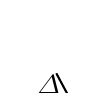
\begin{tikzpicture}
   \node at (0,0){$\Delta$};
   \draw[line width=0.75] (0.25,-0.13) -- (0.1,0.15);
 \end{tikzpicture}
\end{minipage}
}

%Die Modulo-Kommandos in klein, für die Darstellungen unter Quantoren.
\newcommand{\moduloScriptT}[2]{
\mbox{\raisebox{0.4ex}{\scriptsize\ensuremath{\displaystyle #1}}
{\hspace*{-1.5mm}\footnotesize /}
\raisebox{-0.4ex}{\hspace*{-1.5mm}\scriptsize\ensuremath{\displaystyle #2}}
}}

\newcommand{\lmoduloScriptT}[2]{
\mbox{\raisebox{-0.4ex}{\scriptsize\ensuremath{\displaystyle #1}}
{\hspace*{-1.5mm}\footnotesize \ensuremath{\backslash}}
\raisebox{0.4ex}{\hspace*{-1.5mm}\scriptsize\ensuremath{\displaystyle #2}}
}}

\newcommand{\modloScriptT}[2]{\moduloScriptT{ \mathbb{#1}}{#2\mathbb{#1}}}

% stehendes Winkelzeichen
\newcommand{\winkel}{
\begin{tikzpicture}[scale=0.25]
\draw ({-2+3^(1/2)},0) -- (0,1) -- ({2-3^(1/2)},0);
\draw ($(0,1) + ({cos(235)*0.7},{sin(315)*0.7})$) arc (235:315:0.7);
\end{tikzpicture}}

% Wurzel mit Häkchen
\newcommand{\hsqrt}[2][{}]{\setbox0=\hbox{$\sqrt[#1]{\phantom{|}\!\! #2\hspace*{1pt}}$}\dimen0=\ht0
  \advance\dimen0-0.2\ht0
  \setbox2=\hbox{\vrule height\ht0 depth -\dimen0}
  {\box0\lower0.4pt\box2}}

% Damit nicht immer "Kapitel 1" etc. über der Kapitelüberschrift steht
\titleformat{\chapter}
  {\huge\bfseries}
  {\textrm{\thechapter} }{0pt}
  {\textrm{#1} \thispagestyle{fancy}
  }

% Neudefinition der Abschnittsmarker für die Kopfzeile
\renewcommand\partmark[1]{\markboth{#1}{}}
\renewcommand\chaptermark[1]{\markright{\arabic{chapter} #1}}
\renewcommand\sectionmark[1]{}
\renewcommand\subsectionmark[1]{}

% Schriften auf Serif umstellen
\addtokomafont{descriptionlabel}{\rmfamily}
\addtokomafont{disposition}{\rmfamily}

% Kopf- und Fußzeile
% Höhe der Kopfzeile
\setlength{\headheight}{14pt}
% obere Trennlinie
%\renewcommand{\headrulewidth}{0.4pt}
\fancyhf{} %alle Kopf- und Fußzeilenfelder bereinigen
\fancyhead[L]{\textbf{Functional Analysis}} %Kopfzeile links
%\fancyhead[C]{\leftmark} %zentrierte Kopfzeile
\fancyhead[R]{\rightmark} %Kopfzeile rechts
\fancyfoot[C]{\thepage\quad\!\!\!\slash\quad\!\!\!\pageref{END-front}} %Seitenzahl der Front-Matter

\AtBeginDocument{
  \def\labelitemi{\normalfont\bfseries{--}}
  \def\labelitemii{\(\circ\)}
  \def\labelitemiii{\(\triangleright\)}
}

\makeatother

\begin{document}




%Shell-Kommando für Tikz-Externalize:
%pdflatex -shell-escape Functional-Analysis.tex 

\global\long\def\norm#1{\left\lVert #1\right\rVert }


\global\long\def\abs#1{\left\lvert #1\right\rvert }


\global\long\def\opnorm#1{\opnor{#1}}


\global\long\def\BRA#1{\Bra{#1}}


\global\long\def\KET#1{\Ket{#1}}


\global\long\def\BraKet#1{\Braket{#1}}


\global\long\def\mins{\text{-}}


\global\long\def\LB{\LBO}


\global\long\def\exs{\exsop}


\global\long\def\exsg{\exsgop}


\global\long\def\fall{\fallop}


\global\long\def\bcupd{\bcupdop}


\global\long\def\bcapd{\bcapdop}


\global\long\def\sr#1#2#3{\underset{#3}{\overset{#2}{#1}}}


\global\long\def\dd{\textnormal{d}}


\global\long\def\DD{\textnormal{D}}


\global\long\def\TT{\textnormal{T}}


\global\long\def\ii{\textbf{i}}


\global\long\def\modulo#1#2{\moduloT{#1}{#2}}


\global\long\def\lmodulo#1#2{\lmoduloT{#1}{#2}}


\global\long\def\modlo#1#2{\modloT{#1}{#2}}


\global\long\def\moduloScript#1#2{\moduloScriptT{#1}{#2}}


\global\long\def\lmoduloScript#1#2{\lmoduloScriptT{#1}{#2}}


\global\long\def\modloScript#1#2{\modloScriptT{#1}{#2}}


\pagenumbering{roman}


\title{\hspace*{1mm}\vspace*{-15mm}\\
{\Huge Functional Analysis}}


\author{{\small \vspace*{-5mm}}\textit{\small }\\
\textit{\small lecture by}\\
\textit{\noun{\small Prof. Dr. Felix Finster}}\textit{\small }\\
\textit{\small during the winter semester 2012/13}\\
\textit{\small revision and layout in \LyX{} by}\\
\textit{\noun{\small Andreas Völklein}}\\
{\small \vspace*{5mm}}\\
{\small 
\includegraphics[clip,width=15cm]{unir}}\textit{\noun{\small }}\\
{\small \vspace*{3mm}}\\
Last changed: \today\\
{\small \vspace*{-30mm}}}

\maketitle
\fancyhead[R]{License}
\setcounter{page}{2} % sonst gibt es aus irgendeinem Grund zweimal die Seite 1!?


\subsubsection*{ATTENTION}

This script does \emph{not} replace the lecture.\\
Therefore it is recommended \emph{strongly} to attend the lecture.

\vfill{}



\subsubsection*{Copyright Notice}

Copyright © 2012 \noun{Andreas Völklein}

Permission is granted to copy, distribute and/or modify this document
under the terms of the GNU Free Documentation License, Version 1.3
or any later version published by the Free Software Foundation;\\
with no Invariant Sections, no Front-Cover Texts, and no Back-Cover
Texts.\\
A copy of the license is included in the section entitled “GNU Free
Documentation License”.


\subsubsection*{Disclaimer of Warranty}

\noun{Unless otherwise mutually agreed to by the parties in writing
and to the extent not prohibited by applicable law, }\textbf{\noun{the
Copyright Holders and any other party, who may distribute the Document
as permitted above,   provide the Document “as is}}\textbf{”,}\textbf{\noun{
without warranty of any kind}}\noun{, expressed, implied, statutory
or otherwise, including, but not limited to, the implied warranties
of merchantability, fitness for a particular purpose, non-infringement,
the absence of latent or other defects, accuracy, or the absence of
errors, whether or not discoverable.}


\subsubsection*{Limitation of Liability}

\textbf{\noun{In no event}}\noun{ unless required by applicable law
or agreed to in writing }\textbf{\noun{will the Copyright Holders,
or any other party, who may distribute the Document as permitted above,
be liable to you for any damages}}\noun{, including, but not limited
to, any general, special, incidental, consequential, punitive or exemplary
damages, however caused, regardless of the theory of liability, arising
out of or related to this license or any use of or inability to use
the Document, even if they have been advised of the possibility of
such damages.}

\textbf{\noun{In no event will the Copyright Holders'/Distributor's
liability to you}}\noun{, whether in contract, tort (including negligence),
or otherwise, }\textbf{\noun{exceed the amount you paid the Copyright
Holders/Distributor}}\noun{ for the document under this agreement.}


\subsubsection*{Links}

The text of the “GNU Free Documentation License” can also be read
on the following site:
\begin{quote}
\url{https://www.gnu.org/licenses/fdl-1.3.en.html}
\end{quote}
A transparent copy of the recent version of this document can be downloaded
from:
\begin{quote}
\url{https://github.com/andiv/Functional-Analysis}
\end{quote}
\newpage{}

\fancyhead[R]{Literature}


\subsection*{Literature}
\begin{itemize}
\item \noun{Peter D. Lax: }\emph{Functional analysis}; Wiley-Interscience,
2002; ISBN: 0-471-55604-1\emph{}\\
(good reference)
\item \noun{Micheal Reed, Barry Simon}: \emph{Methods of Modern Mathematical
Physics I - Functional Analysis; }Acad. Press, 2010; ISBN: 978-0-12-585050-6
\item \noun{Friedrich Hirzebruch, Winfried Scharlau}: \foreignlanguage{ngerman}{\emph{Einführung
in die Funktionalanalysis}}; Spektrum Verlag, 1996; ISBN: 3-86025-429-4\\
(paperback, small)
\item \noun{Dirk Werner}: \foreignlanguage{ngerman}{\emph{Funktionalanalysis}};
Springer, 2011; ISBN: 978-3-642-21016-7
\item \noun{Joachim Weidmann}: \foreignlanguage{ngerman}{\emph{Lineare Operatoren
in Hilberträumen, Teil I: Grundlagen}}; Teubner, 2000; ISBN: 3-519-02236-2
\item \noun{Walter Rudin}: \emph{Functional Analysis}; McGraw-Hill, 1991;
ISBN: 7-111-13415-X
\end{itemize}
Zorn's Lemma:
\begin{itemize}
\item \noun{Hans-Joachim Kowalsky, Gerhard O. Michler}: \foreignlanguage{ngerman}{\emph{Lineare
Algebra}}; de Gruyter, 2003; ISBN: 3-11-017963-6
\end{itemize}
{\small \newpage{}}\fancyhead[R]{Table of contents}
\fancyhead[C]{}

\tableofcontents{}\label{END-front}\newpage{}\pagenumbering{arabic}
\fancyfoot[C]{\thepage\quad\!\!\!\slash\quad\!\!\!\pageref{END}} % Seitenzahl des Hauptteils%DATE: Do 18.10.2012

\setcounter{chapter}{-1}

\fancyhead[R]{Motivation}
\fancyhead[C]{}


\chapter*{Motivation}

In linear algebra one mainly considers finite-dimensional vector spaces
with additional structures like norm $\norm .$ or scalar product
$\left\langle .,.\right\rangle $.

Let $\left(V,\left\langle .,.\right\rangle \right)$ be a finite-dimensional
scalar product space and $A:V\to V$ a linear map, which is self-adjoint,
that means for all $u,v\in V$:
\begin{align*}
\left\langle Au,v\right\rangle  & =\left\langle u,Av\right\rangle 
\end{align*}



\section*{Theorem \textmd{(orthonormal eigenvector basis)}}

There exists an orthonormal eigenvector basis $\left(u_{i}\right)_{i\in\left\{ 1,\ldots,n\right\} }$,
that means with the eigenvalues $\lambda_{i}\in\mathbb{R}$:
\begin{align*}
\left\langle u_{i},u_{j}\right\rangle  & =\delta_{ij} & Au_{i} & =\lambda_{i}u_{i}
\end{align*}
In infinite dimensions the generalization is the \emph{spectral theorem}.

First reformulate the result from linear algebra:\\
Let $E_{\lambda_{i}}$ be the orthogonal projection operator on the
eigenspace corresponding to $\lambda_{i}$. If this eigenspace is
one dimensional, this means:
\begin{align*}
E_{\lambda_{i}}v & =u_{i}\left\langle u_{i},v\right\rangle =\left|u_{i}\right>\left<u_{i}|v\right>
\end{align*}
Then one can write $A$ as:
\begin{align*}
A & =\sum_{i=1}^{n}\lambda_{i}E_{\lambda_{i}}
\end{align*}



\section*{Theorem \textmd{(spectral theorem)}}

Let $A\in L\left(H\right)$ be a self-adjoint (\foreignlanguage{ngerman}{selbstadjungiert})
operator, then it holds:
\begin{align*}
A & =\int_{\sigma\left(A\right)}\lambda\dd E_{\lambda}
\end{align*}
$\sigma\left(A\right)\subseteq\mathbb{R}$ is the spectrum of $A$
and $E_{\lambda}$ the projection-valued measure (\foreignlanguage{ngerman}{Spektralmaß}).

Applications typically are differential operators, for example:
\begin{align*}
\Delta_{\mathbb{R}^{3}} & =\frac{\partial^{2}}{\partial x_{1}^{2}}+\frac{\partial^{2}}{\partial x_{2}^{2}}+\frac{\partial^{2}}{\partial x_{3}^{2}}
\end{align*}
\begin{align*}
\Delta_{\mathbb{R}^{3}}:C_{0}^{\infty}\left(\mathbb{R}^{3}\right) & \to C^{\infty}\left(\mathbb{R}^{3}\right)\quad\text{linear operator}
\end{align*}
Applications in more detail are studied in the lectures on partial
differential equations I + II.


\chapter{Basic Notions}

\fancyhead[R]{\rightmark}
%\fancyhead[C]{\leftmark}

Let $E$ be a vector space (\foreignlanguage{ngerman}{Vektorraum}),
for example the finite-dimensional vector space $E\simeq\mathbb{R}^{3}$.\\
In the following list the later spaces are special cases of the previous
ones:
\begin{itemize}
\item topological vector spaces
\item metric spaces with a metric $d\left(.,.\right)$ (Polish spaces if
complete)
\item normed spaces with norm $\norm .$ (Banach spaces if complete)
\item scalar product spaces $\left\langle .,.\right\rangle $ (Hilbert spaces
if complete)
\end{itemize}
Let $\mathbb{K}$ be either $\mathbb{R}$ or $\mathbb{C}$.


\section{Definition \textmd{(metric, $\varepsilon$-ball, Cauchy sequence,
complete, Polish space)}}

A map $d:E\times E\to\mathbb{R}$ is called \emph{metric}, if for
all $x,y,z\in E$ holds:
\begin{enumerate}[label=\roman*)]
\item $d\left(x,y\right)=d\left(y,x\right)$ (symmetry)
\item $d\left(x,y\right)\ge0$ and $d\left(x,y\right)=0$ $\Leftrightarrow$
$x=y$ (positive definiteness)
\item $d\left(x,y\right)\le d\left(x,z\right)+d\left(z,y\right)$ (triangle
inequality)
\end{enumerate}
$B_{\varepsilon}\left(x\right):=\left\{ z\in E\big|d\left(x,z\right)<\varepsilon\right\} $
is called \emph{$\varepsilon$-ball}.\\
Consider the topology generated by $B_{\varepsilon}\left(x\right)$:
A set $\Omega\subseteq E$ is open if and only if:
\begin{align*}
\fall_{x\in\Omega}\exs_{\varepsilon\in\mathbb{R}_{>0}} & :B_{\varepsilon}\left(x\right)\subseteq\Omega
\end{align*}
\emph{Completeness}:\\
$\left(x_{n}\right)_{n\in\mathbb{N}}$ is a \emph{Cauchy sequence}
if and only if:
\begin{align*}
\fall_{\varepsilon\in\mathbb{R}_{>0}}\exs_{N\in\mathbb{N}}\fall_{n,m\in\mathbb{N}_{>N}} & :d\left(x_{n},x_{m}\right)<\varepsilon
\end{align*}
$E$ is \emph{complete} if and only if every Cauchy sequence has a
limit.\\
A complete metric space is also called a \emph{Polish space}.


\section{Definition \textmd{(norm, Banach space)}}

Let $\left(E,\norm .\right)$ be a \emph{normed space}, i.e. a $\mathbb{K}$-vector
space with a map $\norm .:E\to\mathbb{R}_{\ge0}$ called \emph{norm}
with the following properties for $x,y\in E$ and $\lambda\in\mathbb{K}$:
\begin{enumerate}[label=\roman*)]
\item $\norm x\ge0$ and $\norm x=0\Leftrightarrow x=0$ (positive definiteness)
\item $\norm{\lambda x}=\abs{\lambda}\cdot\norm x$ (homogeneity)
\item $\norm{u+v}\le\norm u+\norm v$ (triangle inequality)
\end{enumerate}
Define the metric $d\left(x,y\right):=\norm{x-y}$. A complete normed
spaces is called \emph{Banach space}.

Let $A:E\to F$ be a linear map between the Banach spaces $\left(E,\norm ._{E}\right)$
and $\left(F,\norm ._{F}\right)$.


\section{Definition \textmd{(continuous, bounded)}}

$A$ is \emph{continuous} (\foreignlanguage{ngerman}{stetig}) if $A^{-1}\left(\Omega\right)\subseteq E$
is open for all open $\Omega\subseteq F$.\\
$A$ is \emph{bounded} (\foreignlanguage{ngerman}{beschränkt}) if
there exists a $C\in\mathbb{R}_{>0}$ such that for all $u\in E$
holds:
\begin{align*}
\norm{Au}_{F} & \le C\norm u_{E}
\end{align*}



\section{Lemma \textmd{(continuous $\Leftrightarrow$ bounded)}}

$A$ is continuous $\Leftrightarrow$ $A$ is bounded.


\subsubsection*{(no proof)}


\section{Definition \textmd{(dual space, sup-norm)}}

The \emph{dual space} of $E$ is the space of continuous linear mappings
from $E$ to $\mathbb{K}$:
\begin{align*}
E^{*} & =L\left(E,\mathbb{K}\right)
\end{align*}
$L\left(E,F\right)$ is a vector space: For $A,B\in L\left(E,F\right)$,
$\lambda,\mu\in\mathbb{K}$ and $u\in E$ define:
\begin{align*}
\left(\lambda A+\mu B\right)\left(u\right) & :=\lambda A\left(u\right)+\mu B\left(u\right)
\end{align*}
Define also a norm on $L\left(E,F\right)$, which is called \emph{sup-norm}:
\begin{align*}
\norm A & :=\sup_{u\in E,\norm u_{E}\le1}\norm{Au}_{F}
\end{align*}



\section{Theorem}

If $F$ is complete, so is $L\left(E,F\right)$.\\
In particular $E^{*}$ is a Banach space for every $E$.


\subsubsection*{(no proof)}


\chapter{The Hahn-Banach Theorem and Applications}

As a preparation we need Zorn's lemma.


\section{Definition \textmd{(partial ordering, chain, upper bound, maximal)}}

Let $A$ be a set and $\le$ a \emph{partial ordering} (\foreignlanguage{ngerman}{Halbordnung}),
i.e. for all $a,b,c\in A$:
\begin{enumerate}[label=\roman*)]
\item $a\le b$ and $b\le c$ $\Rightarrow$ $a\le c$ (transitivity)
\item $a\le a$ (reflexivity)
\item $a\le b\wedge b\le a\Rightarrow a=b$ (antisymmetry)
\end{enumerate}
\emph{Note}: We do \emph{not} demand that for all $a,b\in A$ holds:
\begin{align*}
\left(a\le b\right)\vee\left(b\le a\right)
\end{align*}
This is a property of a ordering relation.\\
$\left(A,\le\right)$ is called \emph{partially ordered set} (\foreignlanguage{ngerman}{teilweise
geordnete Menge}).\\
A subset $K\subseteq A$ is called \emph{chain} (\foreignlanguage{ngerman}{Kette,
total geordnete Teilmenge}) if for all $x,y\in K$ holds:
\begin{align*}
\left(x\le y\right)\vee\left(y\le x\right)
\end{align*}
An element $u\in A$ is called \emph{upper bound} (\foreignlanguage{ngerman}{obere
Schranke}) of $B\subseteq A$ if $x\le u$ for all $x\in B$.\\
An element $m\in A$ is called \emph{maximal} if $m\le a\in A\Rightarrow m=a$.


\section{Zorn's lemma}

Let $\left(A,\le\right)$ be a partially ordered set in which every
chain has an upper bound. Then there is a maximal element.


\subsubsection*{Proof}

This follows from the axiom of choice, see e.g. Kowalsky: Linear algebra.


\section{Definition \textmd{(sublinear)}}

Let $X$ be a \emph{real} vector space (without topology) and $l:X\to\mathbb{R}$
linear.\\
$p:X\to\mathbb{R}$ is called \emph{sublinear} if for all $x,y\in X$
and $a\in\mathbb{R}_{>0}$:
\begin{enumerate}[label=\roman*)]
\item $p\left(ax\right)=ap\left(x\right)$
\item $p\left(x+y\right)\le p\left(x\right)+p\left(y\right)$
\end{enumerate}
A typical example is $p\left(x\right)=\norm x$, but $p$ does not
need to be positive. Another example is any linear mapping.


\section{Theorem \textmd{(Hahn-Banach, real version, 1927/29)\label{sec:Thm-Hahn-Banach-real}}}

Let $X$ be a real vector space and $Y\subseteq X$ a subspace (\foreignlanguage{ngerman}{Untervektorraum}),
$p:X\to\mathbb{R}$ sublinear and $l:Y\to\mathbb{R}$ linear with
$l\left(y\right)\le p\left(y\right)$ for all $y\in Y$.\\
Then there is a linear extension (\foreignlanguage{ngerman}{Fortsetzung})
$\tilde{l}:X\to\mathbb{R}$ of $l$ to $X$, i.e. $\tilde{l}\big|_{Y}=l$,
such that for all $x\in X$ holds:
\begin{align*}
\tilde{l}\left(x\right) & \le p\left(x\right)
\end{align*}



\subsubsection*{Proof}
\begin{enumerate}[label=\roman*)]
\item Assume $Y\subsetneq X$, since otherwise there is nothing to prove.
Choose a vector $z\in X\setminus Y$. We want to extend $l$ to the
span of $Y$ and $\left\langle z\right\rangle $. $\tilde{l}\left(z\right)$
needs to be prescribed. For all $y\in Y$ and $a\in\mathbb{R}$ holds:
\begin{align*}
\tilde{l}\left(y+az\right) & \stackrel{\text{linearity}}{=}l\left(y\right)+a\tilde{l}\left(z\right)\stackrel{\text{demand}}{\le}p\left(y+az\right)
\end{align*}
If $a=0$, the inequality is clear. By homogeneity assumptions, it
is sufficient to consider the case $a=\pm1$. We thus demand for all
$y,y'\in Y$:
\begin{align*}
l\left(y\right)+\tilde{l}\left(z\right) & \le p\left(y+z\right)\\
l\left(y'\right)-\tilde{l}\left(z\right) & \le p\left(y'-z\right)
\end{align*}
This is equivalent to:
\begin{align*}
l\left(y'\right)-p\left(y'-z\right) & \le\tilde{l}\left(z\right)\le p\left(y+z\right)-l\left(y\right)
\end{align*}
We can choose $\tilde{l}\left(z\right)$ if and only if:
\begin{align*}
l\left(y'\right)-p\left(y'-z\right) & \le p\left(y+z\right)-l\left(y\right)
\end{align*}
(For example set $\tilde{l}\left(z\right)=\sup_{y'\in Y}l\left(y'\right)-p\left(y'-z\right)$.)
\begin{align*}
\Leftrightarrow\quad l\left(y'\right)+l\left(y\right)\stackrel{\text{lineariy}}{=}l\left(y'+y\right) & \le p\left(y+z\right)+p\left(y'-z\right)
\end{align*}
Now prove this inequality:\\
From $y'+y\in Y$ follows that $l\left(y+y'\right)\le p\left(y+y'\right)$
by hypothesis. Moreover, as $p$ is sublinear, it follows:
\begin{align*}
p\left(y+z-z+y'\right) & \le p\left(y'+z\right)+p\left(y'-z\right)
\end{align*}
So the inequality is shown. Thus $l$ can be extended to $Y+\left\langle z\right\rangle $.
\item Consider all extensions:
\begin{align*}
A & :=\left\{ \left(Z,l\right)|Y\subseteq Z\subseteq X\text{ subspace},\ l:Z\to\mathbb{R}\text{ extension of }l_{Y}:Y\to\mathbb{R}\right\} 
\end{align*}
%DATE: Fr 19.10.12\\
This set has a partial ordering $\le$ defined by $\left(Z,l\right)\le\left(Z',l'\right)$
if $Z\subseteq Z'$ and $l'\big|_{Z}=l$.\\
For an index set $I$ (possibly infinite, uncountable) let $K=\left\{ \left(Z_{\nu},l_{\nu}\right)|\nu\in I\right\} $
be a chain, i.e. for all $\left(Z,l\right),\left(Z',l'\right)\in K$:
\begin{align*}
\left(\left(Z,l\right)\le\left(Z',l'\right)\right) & \vee\left(\left(Z',l'\right)\le\left(Z,l\right)\right)
\end{align*}
Set $Z=\bigcup_{\nu\in I}Z_{\nu}$ and define $l:Z\to\mathbb{R}$
by $l\big|_{Z_{\nu}}=l_{\nu}$. (Thus suppose $u\in Z$, so there
is a $\nu\in I$ with $u\in Z_{\nu}$. Set $l\left(u\right):=l_{\nu}\left(u\right)$.
$\nu$ need not be unique. Suppose $u\in Z_{\nu'}$, then we know
that either $Z_{\nu'}\subseteq Z_{\nu}$ and $l_{\nu}\big|_{Z_{\nu'}}=l_{\nu'}$
or $Z_{\nu}\subseteq Z_{\nu'}$ and $l_{\nu'}\big|_{Z_{\nu}}=l_{\nu}$.
In both cases we have $l_{\nu}\left(u\right)=l_{\nu'}\left(u\right)$,
thus $l\left(u\right)$ is well defined.)\\
This $\left(Z,l\right)$ is an upper bound, because for all $\nu\in I$
we have $Z_{\nu}\subseteq Z=\bigcup_{\lambda\in I}Z_{\lambda}$ and
$l$ is an extension of $l_{\nu}$.\\
With Zorn's Lemma follows, that there exists an maximal element $\left(\tilde{Y},\tilde{l}\right)$.

\begin{description}
\item [{Claim:}] $\tilde{Y}=X$
\item [{Proof:}] Otherwise there would be a vector $u\in X\setminus\tilde{Y}$,
and $\tilde{l}$ could be extended to $\tilde{Y}\oplus\left\langle u\right\rangle $,
as shown in i), in contradiction to the maximality of $\tilde{l}$.
Thus $\left(X=\tilde{Y},\tilde{l}\right)$ is the desired extension.\qqed[Claim]
\end{description}
\end{enumerate}
\qqed


\section{Theorem \textmd{(Hahn-Banach, complex version)}}

Let $X$ be a complex vector space and $Y\subseteq X$ a subspace.
Before, we had $l\left(x\right)\le p\left(x\right)$ as condition,
which does not make sense in the complex case, since:
\begin{align*}
l\left(e^{\ii\varphi}x\right) & =e^{\ii\varphi}l\left(x\right)\stackrel{\text{in general}}{\not\in}\mathbb{R}
\end{align*}
Let $p:X\to\mathbb{R}$ be a \emph{seminorm}, i.e.:
\begin{enumerate}[label=\roman*)]
\item $p\left(ax\right)=\abs ap\left(x\right)$ (homogeneity)
\item $p\left(x+y\right)\le p\left(x\right)+p\left(y\right)$ (triangle
inequality)
\end{enumerate}
Let $l:Y\to\mathbb{C}$ be a linear functional with $\abs{l\left(y\right)}\le p\left(y\right)$
for all $y\in Y$.\\
Then $l$ can be extended to $X$ such that $\abs{l\left(x\right)}\le p\left(x\right)$
holds for all $x\in X$.


\subsubsection*{Proof}

We also consider $X$ as a real vector space. ($u$ and $\ii u$ are
then linearly independent vectors.) Decompose $l$ into its real and
imaginary parts.
\begin{align*}
l\left(y\right) & =l_{1}\left(y\right)+\ii l_{2}\left(y\right)\\
l_{1} & :=\text{Re}\left(l\left(y\right)\right)\\
l_{2} & :=\text{Im}\left(l\left(y\right)\right)
\end{align*}
$l_{1}$ and $l_{2}$ are real-linear and:
\begin{align*}
l_{1}\left(\ii y\right) & =\text{Re}\left(l\left(\ii y\right)\right)=\text{Re}\left(\ii l\left(y\right)\right)=-\text{Im}\left(l\left(y\right)\right)=-l_{2}\left(y\right)
\end{align*}
Conversely, suppose that $l_{1}$ is real-linear. Then
\begin{align*}
l\left(x\right) & :=l_{1}\left(x\right)-\ii\cdot l_{1}\left(\ii x\right)
\end{align*}
this is indeed a complex-linear function. We know that $\abs{l\left(y\right)}\le p\left(y\right)$
holds for all $y\in Y$.
\begin{align*}
l_{1}\left(y\right)=\text{Re}\left(l\left(y\right)\right) & \le\abs{l\left(y\right)}\\
\Rightarrow\qquad l_{1}\left(y\right) & \le p\left(y\right)
\end{align*}
Theorem \ref{sec:Thm-Hahn-Banach-real} yields an real-linear extension
$\tilde{l}_{1}:X\to\mathbb{R}$ such that $\tilde{l}_{1}\left(x\right)\le p\left(x\right)$
for all $x\in X$.\\
Set $\tilde{l}\left(x\right)=\tilde{l}_{1}\left(x\right)-\ii\,\tilde{l}_{1}\!\left(\ii x\right)$,
so that $\tilde{l}:X\to\mathbb{C}$ is complex-linear.
\begin{description}
\item [{Claim:}] $\abs{\tilde{l}\left(x\right)}\le p\left(x\right)$ $\fall_{x\in X}$
\item [{Proof:}] Polar decomposition:
\begin{align*}
\tilde{l}\left(x\right) & =re^{\ii\varphi}\\
\abs{\tilde{l}\left(x\right)} & =r=e^{-\ii\varphi}\tilde{l}\left(x\right)\sr ={\tilde{l}\text{ is}}{\text{complex-linear}}\tilde{l}\left(e^{-\ii\varphi}x\right)=\text{Re}\left(\tilde{l}\left(e^{-\ii\varphi}x\right)\right)=\\
 & =\tilde{l}_{1}\left(e^{-\ii\varphi}x\right)\le p\left(e^{-\ii\varphi}x\right)\stackrel{\text{homogeneity}}{=}p\left(x\right)
\end{align*}
\qqed[Claim]
\end{description}
\qqed

Now to applications:


\section{Theorem\label{sec:Thm-HahnBanach-normedSpace}}

Let $\left(X,\norm .\right)$ be a normed $\mathbb{K}$-space (real
or complex), $Y\subseteq X$ a subspace. Let $\varphi$ be a continuous
linear functional from $Y$ to $\mathbb{K}$, i.e. for all $y\in Y$
holds:
\begin{align*}
\abs{\varphi\left(y\right)} & \le\norm{\varphi}\cdot\norm y
\end{align*}
Then $\varphi$ can be continued to all of $X$ with the same supnorm,
i. e.:
\begin{align*}
\norm{\tilde{\varphi}} & :=\sup_{x\in X,\norm x\le1}\abs{\varphi\left(x\right)}=\norm{\varphi}:=\sup_{y\in Y,\norm y\le1}\abs{\varphi\left(y\right)}
\end{align*}



\subsubsection*{Proof}

Apply the Hahn-Banach theorem with $\tilde{\varphi}:=\norm{\varphi}\cdot\norm x$.\qqed


\section{Corollary}

Let $X$ be a normed space and $u_{0}\in X$ with $\norm{u_{0}}=1$.
Then there exists a linear functional $\varphi:X\to\mathbb{K}$ such
that:
\begin{align*}
\varphi\left(u_{0}\right) & =1 & \norm{\varphi} & =1
\end{align*}



\subsubsection*{Proof}

Let $Y:=\left\langle u_{0}\right\rangle $ and define $\varphi_{0}:\left\langle u_{0}\right\rangle \to\mathbb{K}$
by $\varphi_{0}\left(u_{0}\right)=1$. Extend $\varphi_{0}$ by the
Hahn-Banach theorem \ref{sec:Thm-HahnBanach-normedSpace}.\qqed

The Hahn-Banach theorem also has a geometric formulation. Consider
only the real case:\\
A set $K\subseteq X$ is called \emph{convex} if for all $x,y\in K$
and $\tau\in\left[0,1\right]$:
\begin{align*}
\tau x+\left(1-\tau\right)y & \in K
\end{align*}


\begin{figure}[H]
\hfill{}\subfigure[konvex set]{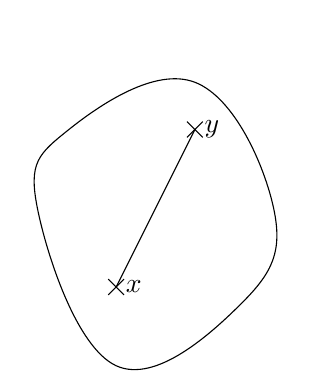
\begin{tikzpicture}[scale=2]
  \draw plot[smooth cycle,tension=.7] coordinates{(0,-1) (0.8,-0.6) (1,0) (0.5,0.8) (-0.3,0.5) (-0.5,0)};
  \draw (0,-0.5) -- (0.5,0.5);
  \draw (0,-0.5) node[right]{$x$} +(-0.05,-0.05) -- +(0.05,0.05) +(0.05,-0.05) -- +(-0.05,0.05);
  \draw (0.5,0.5) node[right]{$y$} +(-0.05,-0.05) -- +(0.05,0.05) +(0.05,-0.05) -- +(-0.05,0.05);
\end{tikzpicture}}\hfill{}\subfigure[concave set]{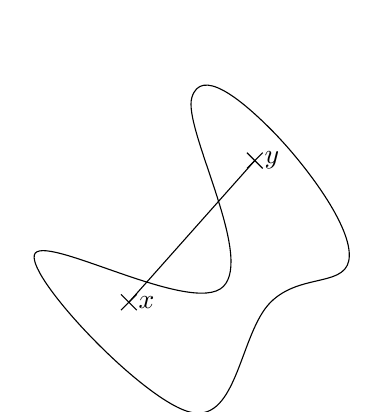
\begin{tikzpicture}[scale=2]
  \draw plot[smooth cycle,tension=.7] coordinates{(0,-1) (0.5,-0.3) (1,0) (0.5,0.8) (0,1) (0.2,-0.2) (-1,0)};
  \draw (-0.4,-0.3) -- (0.4,0.6);
  \draw (-0.4,-0.3) node[right]{$x$} +(-0.05,-0.05) -- +(0.05,0.05) +(0.05,-0.05) -- +(-0.05,0.05);
  \draw (0.4,0.6) node[right]{$y$} +(-0.05,-0.05) -- +(0.05,0.05) +(0.05,-0.05) -- +(-0.05,0.05);
\end{tikzpicture}}\hfill{}\hspace*{1mm}\caption{convexity}


\end{figure}


Geometric question:

\begin{figure}[H]
\hspace*{1mm}\hfill{}\begin{tikzpicture}[scale=2]
  \draw plot[smooth cycle,tension=.7] coordinates{(0,-1) (0.8,-0.6) (1,0) (0.5,0.8) (-0.3,0.5) (-0.5,0)};
  \draw (1.5,0.5) node[right]{$y$} +(-0.05,-0.05) -- +(0.05,0.05) +(0.05,-0.05) -- +(-0.05,0.05);
  \draw[thick,red] (1,1.5) -- (2,-0.5) node[right]{$\mathcal{H}$};
  \node at (0.9,-0.7) {$K$};
\end{tikzpicture}\hfill{}\hspace*{1mm}\caption{not intersecting hyperplane}
\end{figure}


Is there a hyperplane $\mathcal{H}$, which meets $y\not\in K$, but
does not intersect $K$?


\section{Definition \textmd{(interior point)}}

$x_{0}\in K$ is an \emph{interior point} (\foreignlanguage{ngerman}{innerer
Punkt}) \emph{of $K$ with respect to $u\in X$} if there exists an
$\varepsilon\in\mathbb{R}_{>0}$ such that $x_{0}+tu\in K$ for all
$t\in\left(-\varepsilon,\varepsilon\right)$.\\
$x_{0}\in K$ is an \emph{interior point} if for all $u\in X$ there
is a $\varepsilon=\varepsilon\left(u\right)\in\mathbb{R}_{>0}$ such
that $x_{0}+tu\in X$ for all $t\in\left(-\varepsilon,\varepsilon\right)$.


\section{Theorem \textmd{(geometric Hahn-Banach)}\label{sec:Thm-HahnBanach-Geometric}}

Let $K\not=\emptyset$ be convex and all points of $K$ be interior
points. Let $y\not\in K$. Then there is a linear functional $l:X\to\mathbb{R}$
such that $l\left(x\right)<1$ for all $x\in K$ and $l\left(y\right)=1$.\\
$\mathcal{H}:=\left\{ x\in X\big|l\left(x\right)=1\right\} $ defines
a hyperplane. Now $y\in\mathcal{H}$ and $l\big|_{K}<1$ mean that
$K$ lies in one half-space.

First introduce a suitable sublinear functional. Without loss of generality,
assume $0\in K$ (otherwise shift $K$).

\begin{figure}[H]
\hspace*{1mm}\hfill{}\begin{tikzpicture}[scale=2]
  \draw plot[smooth cycle,tension=.7] coordinates{(0,-1) (0.8,-0.6) (1,0) (0.5,0.8) (-0.3,0.5) (-0.5,0)};
  \draw (0,0) node[below]{$0$} +(-0.05,-0.05) -- +(0.05,0.05) +(0.05,-0.05) -- +(-0.05,0.05);
\end{tikzpicture}\hfill{}\hspace*{1mm}\caption{$0\in K$}
\end{figure}


The functional $p:K\to\mathbb{R}_{\ge0}$ with
\begin{align*}
p\left(x\right) & :=\text{inf}\left\{ a\in\mathbb{R}_{>0}\bigg|\frac{x}{a}\in K\right\} 
\end{align*}
is called gauge (\foreignlanguage{ngerman}{Eichung}).\\
Since $x$ is an interior point, we know that $\frac{x}{a}\in K$
if $a>1-\varepsilon\left(x\right)$.\\
$p$ is even defined on all of $X$, because for $x\in X$, now $\tau x\in K$
if $\abs{\tau}$ is sufficiently small, because $0\in K$ is an interior
point.
\begin{align*}
p\left(x\right)<1 & \quad\Leftrightarrow\quad x\in K
\end{align*}


\begin{figure}[H]
\hspace*{1mm}\hfill{}\begin{tikzpicture}[scale=2]
  \draw plot[smooth cycle,tension=.7] coordinates{(0,-1) (0.8,-0.6) (1,0) (0.5,0.8) (-0.3,0.5) (-0.5,0)};
  \draw (0,0) node[below]{$0$} +(-0.05,-0.05) -- +(0.05,0.05) +(0.05,-0.05) -- +(-0.05,0.05);
  \draw (1.5,0.8) node[right]{$x$} +(-0.05,-0.05) -- +(0.05,0.05) +(0.05,-0.05) -- +(-0.05,0.05);
  \draw (0.5,0.2666) node[below right]{$\tau x$} +(-0.05,-0.05) -- +(0.05,0.05) +(0.05,-0.05) -- +(-0.05,0.05);
  \draw[dashed] (1.5,0.8) -- (-0.75,-0.4);
\end{tikzpicture}\hfill{}\hspace*{1mm}\caption{$x\not\in K,\ \tau x\in K$}
\end{figure}



\section{Lemma}

$p$ is sublinear.


\subsubsection*{Proof}

The homogeneity is clear from the definition.

sub-additivity (triangle equation):\\
Take $x,y\in K$ and choose $a,b\in\mathbb{R}_{>0}$ such that $\frac{x}{a},\frac{y}{b}\in K$.
The convexity of $K$ implies for all $\tau\in\left[0,1\right]$:
\begin{align*}
\tau\frac{x}{a}+\left(1-\tau\right)\frac{y}{b} & \in K
\end{align*}
Choose ${\displaystyle \tau=\frac{a}{a+b}}$, then holds ${\displaystyle 1-\tau=\frac{b}{a+b}}$,
which gives:
\begin{align*}
\Rightarrow\quad\frac{1}{a+b}\left(x+y\right) & \in K
\end{align*}
\begin{align*}
p\left(x+y\right) & \le a+b
\end{align*}
Taking the infimum over $a$ and $b$ gives $p\left(x+y\right)\le p\left(x\right)+p\left(y\right)$:
\begin{align*}
p\left(x+y\right) & =\inf\underbrace{\left\{ c\in\mathbb{R}_{>0}\bigg|\frac{x+y}{c}\in K\right\} }_{\ni a+b}\le a+b
\end{align*}
\begin{align*}
p\left(x\right) & =\inf\left\{ a\bigg|\frac{x}{a}\in K\right\} \quad\Rightarrow\quad\fall_{\varepsilon>0}\exs_{a\in\mathbb{R}_{>0}}:p\left(x\right)\ge a-\varepsilon\\
p\left(y\right) & =\inf\left\{ b\bigg|\frac{x}{b}\in K\right\} \quad\Rightarrow\quad\fall_{\varepsilon>0}\exs_{b\in\mathbb{R}_{>0}}:p\left(y\right)\ge b-\varepsilon
\end{align*}
\qqed


\section{Lemma}

$p\left(x\right)<1\Leftrightarrow x\in K$


\subsubsection*{Proof}

If $x\not\in K$ then $\frac{1}{a}x\not\in K$ for all $0<a<1$ and
so $p\left(x\right)\ge1$.

For all $x\in K$ exists an $\varepsilon=\varepsilon\left(x\right)\in\mathbb{R}_{>0}$
with $\left(1+t\right)x\in K$ for all $t\in\left(-\varepsilon,\varepsilon\right)$.
\begin{align*}
\Rightarrow\quad & \left(1+\frac{\varepsilon}{2}\right)x\in K\\
\Rightarrow\quad & p\left(x\right)\le\frac{1}{1+\frac{\varepsilon}{2}}<1
\end{align*}
\qqed


\subsubsection*{Proof of Theorem \ref{sec:Thm-HahnBanach-Geometric}}

Introduce $l$ on $\left\langle y\right\rangle $ by $l\left(y\right)=1$.
(Assume again that $0\in K$ and so $y\not=0$.)\\
Write $z=ay\in\left\langle y\right\rangle $ with $a\in\mathbb{R}$.
\begin{itemize}
\item If $a<0$, then $l\left(z\right)=a\cdot l\left(y\right)=a<0$ but
$p\left(z\right)\ge0$ and thus the inequality $l\left(z\right)\le p\left(z\right)$
is trivially satisfied.
\item If $a>0$ it holds:
\begin{align*}
l\left(z\right) & =a\sr{\le}{y\not\in K}{\Rightarrow p\left(y\right)\ge1}a\cdot p\left(y\right)\sr ={\text{positive}}{\text{homogeneity}}p\left(ay\right)=p\left(z\right)
\end{align*}

\end{itemize}
So for all $z\in\left\langle y\right\rangle $ holds $l\left(z\right)\le p\left(z\right)$.\\
The Hahn-Banach Theorem yields an extension $l:X\to\mathbb{R}$ such
that $l\left(x\right)\le p\left(x\right)$ for all $x\in X$. Therefore
for all $x\in K$ we have:
\begin{align*}
l\left(x\right) & \le p\left(x\right)<1
\end{align*}
\qqed[\ref{sec:Thm-HahnBanach-Geometric}]

%DATE: Do 25.10.12


\chapter{Normed Spaces}

Let $\left(E,\norm .\right)$ be a normed space and let the open balls
$B_{\varepsilon}\left(x\right)=\left\{ y\big|\norm{x-y}<\varepsilon\right\} $
generate the topology on $E$.


\subsection{Definition \textmd{(equivalent norms)}}

Two norms $\norm ._{1}$ and $\norm ._{2}$ are \emph{equivalent},
if there exists a $C\in\mathbb{R}_{>0}$ such that:
\begin{align*}
\frac{1}{C}\norm x_{1} & \le\norm x_{2}\le C\norm x_{2}
\end{align*}



\subsection{Theorem}

Equivalent norms give rise to the same topology.


\subsubsection*{(No proof)}


\subsection{Theorem}

If $E$ is finite dimensional, then any two norms on $E$ are equivalent.


\subsubsection*{(No proof)}


\subsection{Constructions \textmd{(Quotient space, Cartesian product)}}

Let $F\subseteq E$ be a \emph{closed} subspace. Define the \emph{quotient
space }\foreignlanguage{ngerman}{(Faktorraum}) $\modulo EF$ as follows:
\begin{align*}
x\sim y & :\Leftrightarrow x-y\in F
\end{align*}
defines an equivalence relation on $E$.
\begin{align*}
\modulo EF & :=\modulo E{\sim}
\end{align*}
is a vector space.
\begin{align*}
\norm u_{\moduloScript EF} & :=\inf_{\sr{}{\hat{u}\in E}{\hat{u}-u\in F}}\norm{\hat{u}}_{E}
\end{align*}
$\left(\modulo EF,\norm ._{\moduloScript EF}\right)$ is a normed
space. The closedness of $F$ is essential:\\
Suppose $F\subseteq E$ is not closed. Then there exists an $x\in\overline{F}\setminus F$,
thus there is a $\left(x_{n}\right)_{n\in\mathbb{N}}$, $x_{n}\in F$
with $x_{n}\to x$.\\
Let $\left[x\right]\in\modulo EF$ be the equivalence class. Then
$\left[x\right]\not=0$, since $x\not\in F$, but:
\begin{align*}
\norm{\left[x\right]} & =\inf_{\sr{}{\hat{x}\in E}{\hat{x}-x\in F}}\norm{\hat{x}}\stackrel{x-x_{n}\sim x}{\le}\inf\norm{x-x_{n}}=0
\end{align*}
If $\norm ._{\moduloScript EF}$ was a norm, it would imply $\left[x\right]=0$
and thus $x\in F$ in contradiction to $x\in\overline{F}\setminus F$.

Another construction is the \emph{Cartesian product}: Let $E$ and
$F$ be normed spaces.
\begin{align*}
E\times F & :=\left\{ \left(u,v\right)\Big|u\in E,v\in F\right\} 
\end{align*}
\begin{align*}
\norm{\left(u,v\right)}_{E\times F} & :=\norm u_{E}+\norm v_{F}
\end{align*}
is a norm on $E\times F$.


\subsection{Definition \textmd{(separable)}}

A normed space is called \emph{separable}, if there is a countable
dense subset, i.e. there exists a sequence $\left(x_{n}\right)_{n\in\mathbb{N}}$
such that every nonempty open subset of the space contains at least
one element of the sequence.


\subsection{Examples}

The space $\ell^{\infty}$ of bounded sequences $\left(a_{n}\right)_{n\in\mathbb{N}}$,
$a_{n}\in\mathbb{K}$ with $\norm{\left(a_{n}\right)_{n\in\mathbb{N}}}_{\infty}:=\sup_{n}\abs{a_{n}}$
is a Banach space.
\begin{align*}
A & :=\left\{ \left(a_{n}\right)_{n\in\mathbb{N}}\bigg|a_{2n}=0\fall_{n\in\mathbb{N}}\right\} \subseteq\ell^{\infty}
\end{align*}
is a closed subspace.
\begin{align*}
\modulo{\ell^{\infty}}A & \stackrel{\sim}{=}\left\{ \left(a_{n}\right)\bigg|a_{2n+1}=0\fall_{n\in\mathbb{N}}\right\} 
\end{align*}
\begin{align*}
d & :=\left\{ \left(a_{n}\right)\bigg|\exs_{N\in\mathbb{N}}\fall_{n\in\mathbb{N}_{>N}}a_{n}=0\right\} \subseteq\ell^{\infty}
\end{align*}
is a subspace, but not closed in $\ell^{\infty}$. Consider for example
$\left(a_{n}=\frac{1}{n}\right)=:x\in\ell^{\infty}\setminus d$, $x_{n}\in d$
with $x_{n}=\left(a_{n_{l}}\right)_{l\in\mathbb{N}}$ and:
\begin{align*}
a_{n_{l}} & =\begin{cases}
\frac{1}{l} & \text{if }l\le n\\
0 & \text{if }l>n
\end{cases}
\end{align*}
Then converges $x_{n}\to x\not\in d$, and therefore $d$ is not closed.
The closure is:
\begin{align*}
\overline{d} & =\left\{ \left(a_{n}\right)\big|a\xrightarrow{n\to\infty}0\right\} 
\end{align*}
$\ell^{\infty}$ is not separable.


\subsection{Example}

For $1\le p<\infty$ define
\begin{align*}
\ell^{p} & =\left\{ \left(a_{n}\right)_{n\in\mathbb{N}}\bigg|\sum_{n=1}^{\infty}\abs{a_{n}}^{p}<\infty\right\} 
\end{align*}
and the $\ell^{p}$-norm:
\begin{align*}
\norm{\left(a_{n}\right)}_{p} & :=\left(\sum_{n=1}^{\infty}\abs{a_{n}}^{p}\right)^{\frac{1}{p}}
\end{align*}
$\ell^{p}$ is a normed space (Hölder's inequality, Minkowski inequality)
and also separable (see exercises).


\subsection{Example}

Let $\left(\Omega,\mu\right)$ be a measure space (\foreignlanguage{ngerman}{Maßraum}).
\begin{align*}
L^{p}\left(\Omega\right) & \ \left(1\le p<\infty\right) & \norm f_{p} & =\left(\int_{\Omega}\abs{f\left(x\right)}^{p}\dd\mu\right)^{\frac{1}{p}}\\
L^{\infty}\left(\Omega\right) &  & \norm f_{\infty} & =\text{supess}_{\Omega}\abs{f\left(x\right)}=\sup\left\{ L\in\mathbb{R}\big|\mu\left(f^{-1}\left([L,\infty)\right)\right)>0\right\} 
\end{align*}



\section{Non-Compactness of the Unit Ball}

Let $\left(E,\norm .\right)$ be a normed vector space.
\begin{align*}
K & :=\overline{B_{1}\left(0\right)}=\left\{ x\in E\big|\norm x\le1\right\} 
\end{align*}
If $\dim\left(E\right)<\infty$, $K$ is compact by the Heine-Borel
theorem.


\subsection{Theorem\label{sub:Thm-NonCompactUnitBall}}

If $E$ is infinite-dimensional, then $K$ is not sequentially compact
(\foreignlanguage{ngerman}{folgenkompakt}), i.e. it is possible to
construct a sequence $\left(y_{n}\right)$, $y_{n}\in K$, which has
no convergent subsequence.


\subsection{Lemma\label{sub:Lem-d>0.5}}

Let $Y\subsetneq E$ be a proper (\foreignlanguage{ngerman}{echter})
closed subspace. Then there is a $z\in E\setminus Y$ with $\norm z=1$
such that holds:
\begin{align*}
\fall_{y\in Y}:\ \norm{z-y} & >\frac{1}{2}\\
\Leftrightarrow\quad\overline{B_{\frac{1}{2}}\left(z\right)}\cap Y & =\emptyset
\end{align*}


\begin{figure}[H]
\hspace*{1mm}\hfill{}\begin{tikzpicture}[scale=2]
  \draw (0,0) node[above]{$0$} +(-0.05,-0.05) -- +(0.05,0.05) +(0.05,-0.05) -- +(-0.05,0.05);
  \draw (0.542,-0.84) node[right]{$z$} circle (0.5) node[below=30]{$\overline{B}_{\frac{1}{2}}(z)$} +(-0.05,-0.05) -- +(0.05,0.05) +(0.05,-0.05) -- +(-0.05,0.05);
  \draw  (-1,0.3) -- (3,-0.9) node[above]{$Y$};
  \draw[dotted]  (0,0) -- (0.542,-0.84);
  \draw[dashed]  (0.542,-0.84) -- node[below]{$\frac{1}{2}$} (0.042,-0.84);
  \draw (2.5,-1) node[right]{$x$} +(-0.05,-0.05) -- +(0.05,0.05) +(0.05,-0.05) -- +(-0.05,0.05);
  \draw (0.2,-0.31) node[left]{$z'$} +(-0.05,-0.05) -- +(0.05,0.05) +(0.05,-0.05) -- +(-0.05,0.05);
\end{tikzpicture}\hfill{}\hspace*{1mm}\caption{$\overline{B_{\frac{1}{2}}\left(z\right)}\cap Y=\emptyset$}
\end{figure}



\subsubsection*{Proof}

Choose $x\in E\setminus Y\not=\emptyset$. As $E\setminus Y$ is open,
there is a $\delta\in\mathbb{R}_{>0}$ with $B_{\delta}\left(x\right)\cap Y=\emptyset$.
Thus we can define:
\begin{align*}
d:=\inf_{y\in Y}\norm{x-y} & >0
\end{align*}
Choose $y_{0}\in Y$ such that $\norm{x-y_{0}}<2d$. Set $z'=x-y_{0}$.
Then $\norm{z'}<2d$ and $\norm{z'-y}\ge d$ for all $y\in Y$. Thus
$z:=\frac{z'}{\norm{z'}}$ has the desired properties. \qqed


\subsubsection*{Proof of Theorem \ref{sub:Thm-NonCompactUnitBall}}

Choose inductively a sequence $\left(y_{n}\right)$: $y_{1}\in K$
is arbitrary. $Y_{1}:=\left\langle y_{1}\right\rangle $ is a one
dimensional subspace, which is closed. Choose $y_{2}\in K$ such that
$\norm{y_{2}-y}>\frac{1}{2}$ for all $y\in Y_{1}$, which is possible
according to Lemma \ref{sub:Lem-d>0.5}.\\
Suppose $y_{1},\ldots,y_{n}$ are given. $Y_{n}:=\left\langle y_{1},\ldots,y_{n}\right\rangle $
is closed. So there exists a $y_{n+1}\in K$ such that for all $y\in Y_{n}$
holds:
\begin{align*}
\norm{y_{n+1}-y} & >\frac{1}{2}
\end{align*}
This sequence has the following properties:
\begin{itemize}
\item $y_{k}\in K$
\item For all $k,l\in\mathbb{N}$ with $k<l$ holds $\norm{y_{l}-y_{k}}>\frac{1}{2}$,
since $y_{k}\in Y_{l-1}=\left\langle y_{1},\ldots,y_{l-1}\right\rangle $
and we know by construction that $\norm{y_{l}-y}>\frac{1}{2}$ for
all $y\in Y_{l-1}$ so especially for $y_{k}\in Y_{l-1}$.
\end{itemize}
This implies that $\left(y_{k}\right)$ has no convergent subspace.
\qqed[\ref{sub:Thm-NonCompactUnitBall}]


\section{Spaces of linear Mappings, Dual Spaces}

Let $E,F$ be normed spaces.\\
$A:E\to F$ is continuous if and only if it is bounded, i.e. there
exists a $C\in\mathbb{R}_{>0}$ such that for all $u\in E$ holds:
\begin{align*}
\norm{Au}_{F} & \le C\norm u_{E}
\end{align*}
Denote by $L\left(E,F\right)$ the normed space of all bounded linear
maps from $E$ to $F$ and define:
\begin{align*}
\norm A & :=\sup_{\norm u\le1}\norm{Au}=\sup_{\norm u=1}\norm{Au}
\end{align*}



\subsection{Lemma}

If $B\in L\left(E,F\right)$ and $A\in L\left(F,G\right)$ then Schwarz
inequality or Kato inequality holds:
\begin{align*}
\norm{A\cdot B} & \le\norm A\cdot\norm B\\
\norm{Au} & \le\norm A\cdot\norm u
\end{align*}



\subsubsection*{(no proof)}


\subsection{Theorem and Definition \textmd{(dual pairing)\label{sub:TuD-dual-pairing}}}

If $F$ is complete, so is $L\left(E,F\right)$.\\
Special case $F=\mathbb{R}$ and $\norm x_{\mathbb{R}}=\abs x$: $E^{*}:=L\left(E,\,\mathbb{R}\right)$
is the dual space.

For $\varphi\in E^{*}$ and $u\in E$
\begin{align*}
\varphi\left(u\right) & =\left(\varphi,u\right)
\end{align*}
is called \emph{dual pairing} (\foreignlanguage{ngerman}{duale Paarung}).
\begin{align*}
\left(.,.\right):E^{*}\times E & \to\mathbb{R}
\end{align*}
is a continuous bilinear map. For $u\in E$ 
\begin{align*}
\left(.,u\right):E^{*} & \to\mathbb{R}
\end{align*}
defines an element of $E^{**}=L\left(E^{*},\mathbb{R}\right)$. This
gives rise to a linear mapping:
\begin{align*}
\iota:E & \to E^{**}
\end{align*}



\subsubsection*{(no proof)}


\subsection{Theorem}

$\iota:E\hookrightarrow E^{**}$ is an isometric embedding of $E$
into $E^{**}$.


\subsubsection*{Proof}

For $u\in E$ holds:
\begin{align*}
\norm{\iota\left(u\right)} & :=\sup_{\varphi\in E^{*},\norm{\varphi}=1}\norm{\left(\iota\left(u\right)\right)\left(\varphi\right)}=\sup_{\varphi\in E^{*},\norm{\varphi}=1}\norm{\varphi\left(u\right)}\stackrel{?}{=}\norm u
\end{align*}
\begin{align*}
\norm{\varphi} & =\sup_{v\in E,\norm v=1}\abs{\varphi\left(v\right)}
\end{align*}
\begin{align*}
\norm{\varphi\left(u\right)} & \le\norm{\varphi}\cdot\norm u\stackrel{\norm{\varphi}=1}{=}\norm u\\
\Rightarrow\quad\sup_{\varphi\in E^{*},\norm{\varphi}=1}\norm{\varphi\left(u\right)} & \le\norm u
\end{align*}
To prove $\norm{\iota\left(u\right)}\ge\norm u$ apply the Hahn-Banach
theorem:\\
Let $l:\left\langle u\right\rangle \to\mathbb{R}$ be the linear map
with $l\left(u\right)=\norm u$, thus:
\begin{align*}
\norm l & =\sup_{v\in\left\langle u\right\rangle ,\norm v=1}\left(l\left(v\right)\right)=\sup\left(l\left(\pm\frac{u}{\norm u}\right)\right)=1
\end{align*}
By the Hahn-Banach theorem we can extend $l$ to
\begin{align*}
\tilde{l}:E & \to\mathbb{R}
\end{align*}
with $\norm{\tilde{l}}=1$ and then holds:
\begin{align*}
\sup_{\varphi\in E^{*},\norm{\varphi}=1}\varphi\left(u\right) & \stackrel{\norm{\tilde{l}}=1}{\ge}\tilde{l}\left(u\right)=\norm u
\end{align*}
Therefore $\iota$ is injective, because from $\iota\left(u\right)=0$
follows $\norm u_{E}=\norm{\iota\left(u\right)}=0$ and therefore
$u=0$.\qqed


\subsection{Definition \textmd{(reflexive)}}

A Banach space is called \emph{reflexive} (\foreignlanguage{ngerman}{reflexiv})
if $\iota$ is bijective, i.e. $E\stackrel{\sim}{=}E^{**}$.


\subsection{Example}

Let $\ell_{1}$ be the space of absolutely convergent functions with
the norm:
\begin{align*}
\norm{\left(a_{n}\right)}_{1} & =\sum_{n=1}^{\infty}\abs{a_{n}}<\infty
\end{align*}
Let $\left(\lambda_{n}\right)\in\ell_{\infty}$ be a bounded sequence
and define $\Lambda\in\ell_{1}^{*}$:
\begin{align*}
\Lambda:\ell_{1} & \to\mathbb{R}\\
\Lambda\left(\left(a_{n}\right)\right) & =\sum_{n=1}^{\infty}\lambda_{n}a_{n}
\end{align*}
\begin{align*}
\abs{\Lambda\left(\left(a_{n}\right)\right)} & =\abs{\sum_{n=1}^{\infty}\lambda_{n}a_{n}}\le\sum_{n=1}^{\infty}\abs{\lambda_{n}}\cdot\abs{a_{n}}\le\norm{\left(\lambda_{n}\right)}_{\infty}\sum_{n=1}^{\infty}\abs{a_{n}}=\norm{\left(\lambda_{n}\right)}_{\infty}\cdot\norm{\left(a_{n}\right)}_{1}<\infty
\end{align*}
Thus $\Lambda$ is bounded and:
\begin{align*}
\norm{\Lambda} & =\sup_{n\in\mathbb{N}}\abs{\lambda_{n}}
\end{align*}
%DATE: Fr 26.10.12
\begin{description}
\item [{Claim:}] Every bounded linear functional on $\ell_{1}$ is of this
form, i.e. $\ell_{1}^{*}=\ell_{\infty}$.
\item [{Proof:}] Let $\Lambda\in\ell_{1}^{*}$. Choose $u_{l}\in\ell_{1}$
by $u_{l}=\left(0,\ldots,0,1,0,\ldots\right)$ with a one at the $l$-th
position. Setting $\lambda_{l}:=\Lambda\left(u_{l}\right)$ gives:
\begin{align*}
\abs{\lambda_{l}} & =\abs{\Lambda\left(u_{l}\right)}\le\underbrace{\norm{\Lambda}}_{<\infty}\cdot\underbrace{\norm{u_{l}}}_{=1}\le\norm{\Lambda}<\infty
\end{align*}
So $\left(\lambda_{l}\right)\in\ell_{\infty}$.\\
Let $\left(a_{k}\right)$ be a finite sequence, with only zeros for
$k>K\in\mathbb{N}$. Then:
\begin{align*}
\Lambda\left(\left(a_{k}\right)\right) & =\Lambda\left(\sum_{k=1}^{K}a_{k}u_{k}\right)=\sum a_{k}\Lambda\left(u_{k}\right)=\sum\lambda_{k}a_{k}
\end{align*}
Since the finite sequences are dense in $\ell_{1}$, the claim follows.
\qqed[Claim]
\end{description}
So $\ell_{1}^{*}=\ell_{\infty}$ and one could assume $\ell_{\infty}^{*}=\ell_{1}$,
but this is not the case (see exercises).

Thus $\ell_{1}^{**}\not=\ell_{1}$, which means, that $\ell_{1}$
is \emph{not} reflexive.


\section{Weak Convergence \textmd{(Schwache Konvergenz)}}

Let $E$ be a Banach space and $\left(u_{n}\right)$ a sequence in
$E$.

Normal convergence: $u_{n}\to u$ if and only if $\norm{u-u_{n}}\xrightarrow{n\to\infty}0$.


\subsection{Definition \textmd{(weak convergence, weak Cauchy sequence)}}

A sequence $\left(u_{n}\right)$ in $E$ \emph{converges weakly} to
$u$, written as $u_{n}\rightharpoondown u$, if for all $\varphi\in E^{*}$
the sequence $\varphi\left(u_{n}\right)$ converges to $\varphi\left(u\right)$,
i.e. $\varphi\left(u_{n}\right)\to\varphi\left(u\right)$.

$\left(u_{n}\right)$ is a \emph{weak Cauchy sequence} if for all
$\varphi\in E^{*}$ the sequence $\varphi\left(u_{n}\right)$ is a
Cauchy sequence.


\subsection{Theorem \textmd{(Uniqueness of weak limit)}}

The weak limit is unique.


\subsubsection*{Proof}

Let $\left(u_{n}\right)$ be a sequence in $E$, which converges weakly
to $u$ and $u'$, i.e. for all $\varphi\in E^{*}$ holds:
\begin{align*}
\varphi\left(u_{n}\right) & \to\varphi\left(u\right) & \varphi\left(u_{n}\right) & \to\varphi\left(u'\right)
\end{align*}
\begin{align*}
\Rightarrow\quad0=\varphi\left(u_{n}-u_{n}\right) & \to\varphi\left(u-u'\right)
\end{align*}
So $\varphi\left(u-u'\right)=0$ for all $\varphi\in E^{*}$.
\begin{description}
\item [{Claim:}] $v:=u-u'=0$
\item [{Proof:}] Assume to the contrary that $v\not=0$.\\
Choose $\varphi:\left\langle v\right\rangle \to\mathbb{R}$ with $\varphi\left(v\right)=1$.
By the Hahn-Banach theorem $\varphi$ can be extended continuously
to $E$.\\
Therefore exists a $\varphi\in E^{*}$ with $\varphi\left(v\right)=1$,
which is a contradiction to $\varphi\left(v\right)=0$.\qqed[Claim]
\end{description}
\qqed


\subsection{Theorem \textmd{(convergence implies weak convergence)}}

Every convergent sequence converges weakly.


\subsubsection{Proof}

Suppose that $u_{n}\to u$. For $\varphi\in E^{*}$ follows:
\begin{align*}
\abs{\varphi\left(u_{n}\right)-\varphi\left(u\right)} & =\abs{\varphi\left(u_{n}-u\right)}\le\underbrace{\norm{\varphi}}_{\in\mathbb{R}}\cdot\norm{u_{n}-u}\to0
\end{align*}
\begin{align*}
\Rightarrow\quad\varphi\left(u_{n}\right) & \to\varphi\left(u\right)\\
\Rightarrow\quad u_{n} & \rightharpoondown u
\end{align*}
\qqed


\subsection{Example}

$E=\left\{ \left(a_{n}\right)\bigg|a_{n}\xrightarrow{n\to\infty}0\right\} \subsetneq\ell_{\infty}$
with $\norm{\left(a_{n}\right)}=\sup_{n}\abs{a_{n}}$ is a Banach
space.\\
Let $u_{n}=\left(0,\ldots,0,1,0,\ldots\right)$ be the sequence with
a one at the $n$-th position and zeros elsewhere. For $n\not=m$
we have:
\begin{align*}
\norm{u_{n}-u_{m}} & =\sup\left\{ 0,\abs 1,\abs{-1}\right\} =1
\end{align*}
Thus $\left(u_{n}\right)$ is \emph{not} a Cauchy sequence. Every
$\varphi\in E^{*}$ can be represented with $\left(\lambda_{k}\right)\in\ell_{1}$
as (see exercises):
\begin{align*}
\varphi\left(\left(a_{n}\right)\right) & =\sum_{k}\lambda_{k}a_{k}\\
\norm{\varphi} & =\sum_{k=1}^{\infty}\abs{\lambda_{k}}<\infty
\end{align*}
\begin{align*}
\varphi\left(u_{n}\right) & =\sum_{k=1}^{\infty}\lambda_{k}\delta_{kn}=\lambda_{n}\xrightarrow{n\to\infty}0
\end{align*}
From $\left(\lambda_{n}\right)\in\ell_{1}$ follows $\lambda_{n}\to0$.
This means that $u_{k}\rightharpoondown0$.\\
This is used in the lectures on partial differential equations.\\
From $\mathscr{S}\left(u_{n}\right)\to\inf\mathscr{S}$ follows not
necessarily $u_{n}\to u$, but $u_{n}\rightharpoondown u$.

Consider $A_{n}\in L\left(E,F\right)$.
\begin{itemize}
\item \emph{norm convergence}: $A_{n}\to A$ in $L\left(E,F\right)$ means
$\norm{A_{n}-A}\to0$.
\item \emph{strong convergence}: $A_{n}u\to Au$ in $F$ for all $u\in E$.
\item \emph{weak convergence}: $A_{n}u\rightharpoondown Au$ for all $u\in E$,
i.e. for all $\varphi\in F^{*}$ holds $\varphi\left(A_{n}u\right)\to\varphi\left(Au\right)$.
\end{itemize}

\section{The Baire Category Theorem}

Let $E$ be a metric space (e.g. a normed space).


\subsection{Definition \textmd{(nowhere dense, set of first/second category)}}

A subset $A\subseteq E$ is called \emph{nowhere dense} (\foreignlanguage{ngerman}{nirgends
dicht}) if $\overline{A}^{\circ}=\emptyset$.\\
$A$ is called \emph{of first category} (or \emph{meager}) if it can
be written as a countable union of nowhere dense sets. Otherwise it
is \emph{of second category}.


\subsubsection*{Example}
\begin{itemize}
\item $\mathbb{N}\subseteq\mathbb{R}$ is nowhere dense: $\overline{\mathbb{N}}=\mathbb{N}$,
$\mathbb{N}^{\circ}\:=\emptyset$
\item $\mathbb{Q}\subseteq\mathbb{R}$ is dense: $\overline{\mathbb{Q}}=\mathbb{R}$,
$\overline{\mathbb{Q}}^{\circ}=\mathbb{R}^{\circ}=\mathbb{R}$
\end{itemize}

\subsection{Theorem \textmd{(René Baire, 1899)\label{sub:Thm-Baire}}}

Let $E\not=\emptyset$ be a complete metric space (Polish space).
Then $E$ is of second category.


\subsubsection*{Proof}

\begin{figure}[h]
\hspace*{1mm}\hfill{}\begin{tikzpicture}
  % n=1
  \draw (0,0) circle (4);
  \node at (3.1,3.1) {$\overline{B_1}$};
  \draw (-4, -5) -- (7,-3) node[right]{$M_1$};
  \draw (2.5,-1) node[right]{$x_1$}  +(-0.1,-0.1) -- +(0.1,0.1) +(0.1,-0.1) -- +(-0.1,0.1);
  % n=2
  \draw (1,1) circle (2);
  \draw (1,1)  +(-0.1,-0.1) -- +(0.1,0.1) +(0.1,-0.1) -- +(-0.1,0.1);
  \draw[dotted] (1,1) -- node[above]{$r_2$} (-1,1);
  \node at (2,3) {$\overline{B_2}$};
  \draw (-4, -2) -- (7,-2) node[right]{$M_2$};
  \draw (1.7,1.3) node[right]{$x_2$}  +(-0.1,-0.1) -- +(0.1,0.1) +(0.1,-0.1) -- +(-0.1,0.1);
  % n --> Infinity
  \draw[red] (0.7,1.8) node[right]{$x_0$}  +(-0.1,-0.1) -- +(0.1,0.1) +(0.1,-0.1) -- +(-0.1,0.1);
  \draw (0.9,1.9) circle (0.5) node[above right=6] {$\overline{B_3}$};
\end{tikzpicture}\hfill{}\hspace*{1mm}\caption{$B_{n}\cap M_{n}=\emptyset$}
\end{figure}


Assume in contrast that $E=\bigcup_{n\in\mathbb{N}}M_{n}$ and the
sets $M_{n}$ are nowhere dense. Without loss of generality assume
that the $M_{n}$ are closed, since otherwise one can replace $M_{n}$
by $\overline{M_{n}}$.\\
We shall construct inductively balls $\overline{B_{n}}=\overline{B_{r_{n}}\left(x_{n}\right)}$
such that $\overline{B_{n+1}}\subseteq\overline{B_{n}}$, $r_{n}<2^{-n}$
and $\overline{B_{n}}\cap M_{n}=\emptyset$ for all $n$.

Then the points $x_{n}$ form a Cauchy sequence, because for all $n<m\in\mathbb{N}$
we have $x_{n+1}\in B_{n}$ and so $\norm{x_{n}-x_{n+1}}<r_{n}<2^{-n}$:
\begin{align*}
\norm{x_{n}-x_{m}} & \le\norm{x_{n}-x_{n+1}}+\norm{x_{n+1}-x_{m}}\le\ldots\le\\
 & \le2^{-n}+2^{-\left(n+1\right)}+\ldots+2^{-\left(m-1\right)}\le2^{-n}\left(1+\frac{1}{2}+\frac{1}{4}+\ldots\right)\le2\cdot2^{-n}
\end{align*}
Since $E$ is complete, $x_{n}\to x_{0}\in E$ converges. Then $x_{0}\in\overline{B_{n}}$
for all $n$, which implies $x_{0}\not\in M_{n}$ and thus the contradiction
$x_{0}\not\in\bigcup_{n}M_{n}=E$ follows.

Construction of the balls $\overline{B_{n}}$:\\
$M_{1}$ is nowhere dense and therefore $B_{1}\left(0\right)\not\subseteq M_{1}$.
So there exists a $x_{1}\in B_{1}\left(0\right)\setminus M_{1}$.
Since $M_{1}$ is closed, $B_{1}\left(0\right)\setminus M_{1}$ is
open and therefore there exists a radius $r_{1}$ such that $B_{2r_{1}}\left(x_{1}\right)$
is contained in $B_{1}\left(0\right)\setminus M_{1}$ and thus $\overline{B_{r_{1}}\left(x_{1}\right)}\cap M_{1}=\emptyset$.

Suppose $\overline{B_{n}}$ has been constructed. $M_{n+1}$ is nowhere
dense and closed and so there exists a $x_{n+1}\in\overline{B_{n}}\setminus M_{n+1}$
and $r_{n+1}<2^{-\left(n+1\right)}$ such that $B_{2r_{n+1}}\left(x_{n+1}\right)\subseteq\overline{B_{n}}\setminus M_{n+1}$.
Then follows $\overline{B_{r_{n+1}}\left(x_{n+1}\right)}\cap M_{n+1}=\emptyset$.\qqed


\subsection{Theorem \textmd{(Uniform boundedness principle, }\foreignlanguage{ngerman}{\textmd{Prinzip
der gleichmäßigen Beschränktheit}}\textmd{)\label{sub:Thm-Uniform-boundedness}}}

Let $E$ be a Banach space and $F$ a normed space. Let $T_{i}$ be
a sequence in $L\left(E,F\right)$ which is point-wise bounded, i.e.
for all $u\in E$:
\begin{align*}
\sup_{i}\norm{T_{i}u} & \le C\left(u\right)<\infty
\end{align*}
Then sup-norms of $T_{i}$ are bounded:
\begin{align*}
\sup_{i}\norm{T_{i}} & =\sup_{i}\sup_{\norm u=1}\norm{T_{i}u}\le\tilde{C}<\infty
\end{align*}
(Thus there exists a constant $C\in\mathbb{R}_{>0}$ such that $\norm{T_{i}u}\le C$
for all $i\in\mathbb{N}$ and for all $u\in E$ with $\norm u=1$.)


\subsubsection*{Proof}

The sets $M_{n}=\left\{ u\in E\big|\sup_{i}\norm{T_{i}u}\le n\right\} $
are closed by continuity of the $T_{i}\in L\left(E,F\right)$, i.e.
for $u_{k}\to u$ converges $\norm{T_{i}u_{k}}\xrightarrow{k\to\infty}\norm{T_{i}u}$.\\
$E=\bigcup_{n}M_{n}$, because for any $u\in E$, $\sup_{i}\norm{T_{i}u}<\infty$
and thus $u\in M_{n}$ for $n>\sup_{i}\norm{T_{i}u}$.\\
If all the sets $M_{n}$ had empty interior, we would get a contradiction
to Baire's theorem.\\
So there exists an $n_{0}\in\mathbb{N}$ such that $\stackrel{\circ}{M_{n_{0}}}\not=\emptyset$
and thus there are $u_{0}\in E$ and $r\in\mathbb{R}_{>0}$ such that
$B_{r}\left(u_{0}\right)\subseteq M_{n_{0}}$.

\begin{figure}[h]
\hspace*{1mm}\hfill{}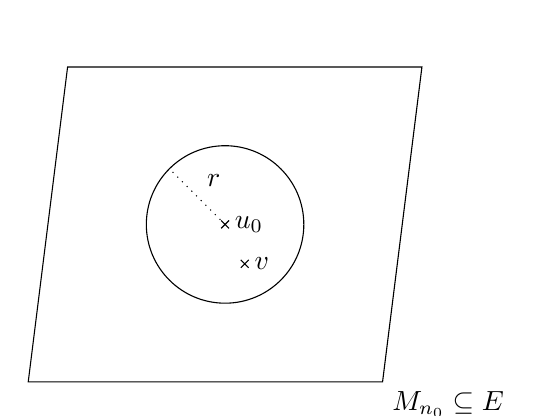
\begin{tikzpicture}[scale=0.5]
  \draw (0,0) circle (2);
  \draw (0,0) node[right]{$u_0$}  +(-0.1,-0.1) -- +(0.1,0.1) +(0.1,-0.1) -- +(-0.1,0.1);
  \draw[dotted] (0,0) -- node[above right]{$r$} (-1.41,1.41);
  \draw (0.5,-1) node[right]{$v$}  +(-0.1,-0.1) -- +(0.1,0.1) +(0.1,-0.1) -- +(-0.1,0.1);
  \draw (-5,-4) -- (4,-4) node[below right]{$M_{n_0}\subseteq E$} -- (5,4) -- (-4,4) -- cycle;
\end{tikzpicture}\hfill{}\hspace*{1mm}\caption{$B_{r}\left(u_{0}\right)\subseteq M_{n_{0}}$}
\end{figure}


For all $v\in B_{r}\left(u_{0}\right)$ we know that $\sup_{i}\norm{T_{i}v}\le n_{0}$
which is equivalent to:
\begin{align*}
\sup_{v\in B_{r}\left(u_{0}\right)}\norm{T_{i}v} & \le n_{0}\qquad\fall_{i\in\mathbb{N}}
\end{align*}
Let $w\in B_{r}\left(0\right)$ be arbitrary. Then $v:=u_{0}+w\in B_{r}\left(u_{0}\right)$.
\begin{align*}
T_{i}w & \stackrel{T_{i}\text{ linear}}{=}T_{i}v-T_{i}u_{0}
\end{align*}
\begin{align*}
\norm{T_{i}w} & \le\norm{T_{i}v}+\norm{T_{i}u_{0}}\le n_{0}+\sup_{i}\norm{T_{i}u_{0}}<\infty
\end{align*}
Here $\sup_{i}\norm{T_{i}u_{0}}<\infty$, because the $T_{i}$ are
point-wise bounded.
\begin{align*}
\Rightarrow\quad\norm{T_{i}w} & \le C\qquad\fall_{w\in B_{r}\left(0\right)}\\
\Rightarrow\quad\norm{T_{i}\tilde{w}} & \le\tilde{C}=\frac{C}{r}\qquad\fall_{\tilde{w}\in\overline{B_{1}\left(0\right)}}
\end{align*}
So $\norm{T_{i}}\le\tilde{C}$ for all $i\in\mathbb{N}$ and so $\norm{T_{i}}$
is bounded.\qqed


\subsection{Corollary}

Let $E$ be a normed space, not necessarily complete, and $\left(u_{n}\right)$
a weak Cauchy sequence. Then $\norm{u_{n}}$ is a bounded sequence.


\subsubsection*{Proof}

$E^{*}=L\left(E,\mathbb{R}\right)$ is a Banach space after theorem
\ref{sub:TuD-dual-pairing}, since $\mathbb{R}$ is complete. Now
we can view every $u_{n}$ as operator:
\begin{align*}
u_{n}:E^{*} & \to\mathbb{R}\\
\varphi & \mapsto\varphi\left(u_{n}\right)
\end{align*}
So $\left(u_{n}\right)$ is a sequence in $L\left(E^{*},\mathbb{R}\right)$.
For all $\varphi\in E^{*}$ we know that $\varphi\left(u_{n}\right)$
is a Cauchy sequence and thus bounded:
\begin{align*}
\Rightarrow\quad\abs{\varphi\left(u_{n}\right)} & <C\left(\varphi\right)
\end{align*}
Applying theorem \ref{sub:Thm-Uniform-boundedness} yields:
\begin{align*}
\abs{\varphi\left(u_{n}\right)} & <C\quad\fall_{\varphi\text{ with }\norm{\varphi}=1}\\
\Leftrightarrow\quad\sup_{n\in\mathbb{N}}\ \sup_{\varphi\in E^{*},\norm{\varphi}=1}\abs{\varphi\left(u_{n}\right)} & <C
\end{align*}
For any $v\in E$ we have
\begin{align*}
\sup_{\varphi\in E^{*},\norm{\varphi}=1}\abs{\varphi\left(v\right)} & =\norm v
\end{align*}
by the Hahn-Banach theorem:
\begin{itemize}
\item $\abs{\varphi\left(v\right)}\le\norm{\varphi}\cdot\norm v\stackrel{\norm{\varphi}=1}{=}\norm v$
\item Choose $\varphi:\left\langle v\right\rangle \to\mathbb{R}$ with $\varphi\left(v\right)=\norm v$
and so $\norm{\varphi}=1$. By the Hahn-Banach theorem we can extend
$\varphi$ to $\tilde{\varphi}:E\to\mathbb{R}$ such that $\norm{\tilde{\varphi}}=1$.
Then $\tilde{\varphi}\left(v\right)=\norm v$ and so $\sup_{\norm{\varphi}=1}\abs{\varphi\left(v\right)}\ge\norm v$.
\end{itemize}
Thus we get $\sup_{n}\norm{u_{n}}<C$.\qqed

%DATE: Fr 2.11.12


\subsection{Corollary and Definition \textmd{(Banach-Steinhaus, equicontinuous,
uniformly continuous)}}

Let $E,F$ be Banach spaces and $T_{i}\in L\left(E,F\right)$.

If the $\left(T_{i}\right)$ are point-wise bounded, then the $T_{i}$
are \emph{equicontinuous} (\foreignlanguage{ngerman}{gleichgradig
stetig}).


\subsubsection{Definition \textmd{(uniformly continuous, equicontinuous)}}

Let $f:\mathbb{R}\to\mathbb{R}$ be a real-valued function.

Continuity:
\begin{align*}
\fall_{x_{0}\in\mathbb{R}}\ \fall_{\varepsilon\in\mathbb{R}_{>0}}\ \exs_{\delta\in\mathbb{R}_{>0}}:\quad & \abs{x-x_{0}}<\delta\quad\Rightarrow\quad\abs{f\left(x\right)-f\left(x_{0}\right)}<\varepsilon
\end{align*}
 $f$ is called \emph{uniformly continuous} (\foreignlanguage{ngerman}{gleichmäßig
stetig}) if:
\begin{align*}
\fall_{\varepsilon\in\mathbb{R}_{>0}}\ \exs_{\delta\in\mathbb{R}_{>0}}: & \quad\norm{x-y}<\delta\quad\Rightarrow\quad\norm{f\left(x\right)-f\left(y\right)}<\varepsilon
\end{align*}
Let $f_{n}:\mathbb{R}\to\mathbb{R}$ be a series of real-valued functions.
$\left(f_{n}\right)$ is called \emph{equicontinuous} if: 
\begin{align*}
\fall_{x_{0}\in\mathbb{R}}\ \fall_{\varepsilon\in\mathbb{R}_{>0}}\ \exs_{\delta\in\mathbb{R}_{>0}}\ \fall_{n\in\mathbb{N}}: & \quad\norm{x-x_{0}}<\delta\quad\Rightarrow\quad\norm{f_{n}\left(x\right)-f_{n}\left(x_{0}\right)}<\varepsilon
\end{align*}
For a linear map $A\in L\left(E,F\right)$ holds:
\begin{align*}
\norm{Au} & \le\norm A\norm u\\
\norm{Au-Au_{0}} & \le\norm A\norm{u-u_{0}}
\end{align*}
Therefore choose $\delta=\frac{\varepsilon}{2\norm A}$, i.e.:
\begin{align*}
\fall_{\varepsilon\in\mathbb{R}_{>0}}\ \exs_{\delta\in\mathbb{R}_{>0}}: & \quad\norm u<\delta\quad\Rightarrow\quad\norm{Au}<\varepsilon
\end{align*}



\subsubsection*{Proof}

Since $\left(T_{i}\right)$ is point-wise bounded there is a $C\in\mathbb{R}_{>0}$
such that for all $i\in\mathbb{N}$ holds $\norm{T_{i}}\le C$ due
to the principle of uniform boundedness \ref{sub:Thm-Uniform-boundedness}.
So for all $i\in\mathbb{N}$ holds:
\begin{align*}
\norm{T_{i}u} & \le\norm{T_{i}}\norm u\le C\norm u
\end{align*}
Choose $\delta=\frac{\varepsilon}{2C}$ shows that the $T_{i}$ is
equicontinuous.\qqed

In the following let $E$ and $F$ be Banach spaces.


\subsection{Definition \textmd{(open)}}

A (not necessarily linear) map $A:E\to F$ is called \emph{open} if
the image of every open set is open. (If there exists an inverse $A^{-1}$
then ``$A$ open'' is equivalent to ``$A^{-1}$ continuous''.)

Let $A$ be linear and open. $B_{1}\left(0\right)\subseteq E$ is
open, so $A\left(B_{1}\left(0\right)\right)\subseteq F$ is open.\\
Since $0\in A\left(B_{1}\left(0\right)\right)$, there is a $\varepsilon\in\mathbb{R}_{>0}$
such that $B_{\varepsilon}\left(0\right)\subseteq A\left(B_{1}\left(0\right)\right)$.

\begin{figure}[h]
\hspace*{1mm}\hfill{}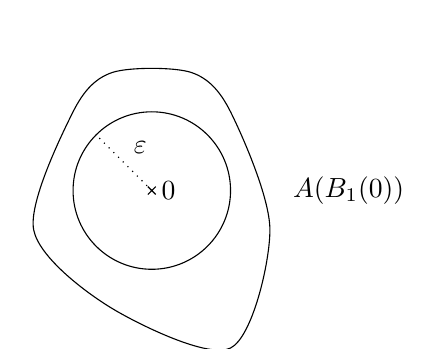
\begin{tikzpicture}[scale=0.5]
  \draw (0,0) circle (2);
  \draw (0,0) node[right]{$0$}  +(-0.1,-0.1) -- +(0.1,0.1) +(0.1,-0.1) -- +(-0.1,0.1);
  \draw[dotted] (0,0) -- node[above right]{$\varepsilon$} (-1.41,1.41);
  \draw plot[smooth cycle] coordinates {(-3,-1) (-1,-3) (2,-4) (3,-1) (2,2) (1,3) (-1,3) (-2,2)};
  \node at (5,0) {$A(B_1(0))$};
\end{tikzpicture}\hfill{}\hspace*{1mm}\caption{$B_{\varepsilon}\left(0\right)\subseteq A\left(B_{1}\left(0\right)\right)$}
\end{figure}


Due to the linearity holds in general:
\begin{align*}
B_{\lambda}\left(0\right) & \subseteq A\left(B_{\frac{\lambda}{\varepsilon}}\left(0\right)\right)
\end{align*}
In particular, $A$ is surjective.

If $A$ is additionally injective, then $A$ is bijective and the
openness means that $A^{-1}$ is continuous.


\subsection{Theorem \textmd{(Open mapping theorem, }\foreignlanguage{ngerman}{\textmd{Prinzip
der offenen Abbildung}}\textmd{)\label{sub:Thm-Open-mapping}}}

If $A\in L\left(E,F\right)$ is surjective, then $A$ is open.


\subsection{Corollary}

If $A\in L\left(E,F\right)$ is bijective, then $A^{-1}\in L\left(F,E\right)$
is continuous.


\subsubsection*{Proof}

Since $A$ is surjective, from \ref{sub:Thm-Open-mapping} follows
that $A$ is open, which means that $A^{-1}$ is continuous.\qqed


\subsubsection*{Proof of \ref{sub:Thm-Open-mapping}}

Since $A$ is surjective, $F=A\left(E\right)$. Since every element
of $E$ has a finite norm, we know:
\begin{align*}
E & =\bigcup_{n\in\mathbb{N}}B_{n}\left(0\right)\\
\Rightarrow\quad F & =A\left(\bigcup_{n\in\mathbb{N}}B_{n}\left(0\right)\right)=\bigcup_{n\in\mathbb{N}}A\left(B_{n}\left(0\right)\right)
\end{align*}
According to Baire's theorem there is a $n\in\mathbb{N}$ such that
$\overline{A\left(B_{n}\left(0\right)\right)}^{\,\circ}\not=\emptyset$.

\begin{figure}[h]
\hspace*{1mm}\hfill{}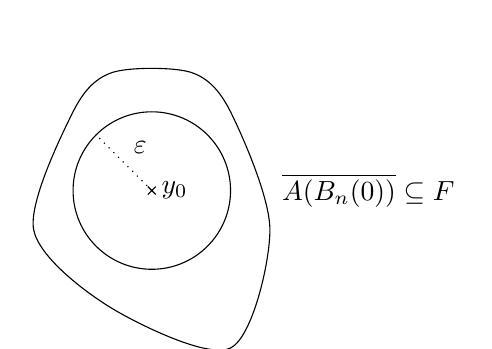
\begin{tikzpicture}[scale=0.5]
  \draw (0,0) circle (2);
  \draw (0,0) node[right]{$y_0$}  +(-0.1,-0.1) -- +(0.1,0.1) +(0.1,-0.1) -- +(-0.1,0.1);
  \draw[dotted] (0,0) -- node[above right]{$\varepsilon$} (-1.41,1.41);
  \draw plot[smooth cycle] coordinates {(-3,-1) (-1,-3) (2,-4) (3,-1) (2,2) (1,3) (-1,3) (-2,2)};
  \node at (5.5,0) {$\overline{A(B_n(0))}\subseteq F$};
\end{tikzpicture}\hfill{}\hspace*{1mm}\caption{$B_{\varepsilon}\left(y_{0}\right)\subseteq\overline{A\left(B_{n}\left(0\right)\right)}$}
\end{figure}


So there exists a $y_{0}\in A\left(B_{n}\left(0\right)\right)$ and
a $\varepsilon\in\mathbb{R}_{>0}$ such that $B_{\varepsilon}\left(y_{0}\right)\subseteq\overline{A\left(B_{n}\left(0\right)\right)}$.
Since $A$ is surjective, there is a $x_{0}\in B_{n}\left(0\right)$
with $y_{0}=A\left(x_{0}\right)$.
\begin{align*}
\Rightarrow\quad\overline{A\left(B_{n}\left(0\right)-x_{0}\right)} & =\overline{A\left(B_{n}\left(0\right)\right)-y_{0}}=\overline{A\left(B_{n}\left(0\right)\right)}-y_{0}\supseteq B_{\varepsilon}\left(y_{0}\right)-y_{0}=B_{\varepsilon}\left(0\right)
\end{align*}
If $n'$ is large enough, then $B_{n}\left(-x_{0}\right)\subseteq B_{n'}\left(0\right)$
and so $\overline{A\left(B_{n'}\left(0\right)\right)}\supseteq B_{\varepsilon}\left(0\right)$.\\
Since $A$ is linear, we can rescale, i.e. there is a $c:=\frac{\varepsilon}{n'}\in\mathbb{R}_{>0}$
such that for all $r\in\mathbb{R}_{<0}$ holds:
\begin{align*}
\overline{A\left(B_{r}\left(0\right)\right)} & \supseteq B_{cr}\left(0\right)
\end{align*}
Now we show that every $u\in B_{c}\left(0\right)$ is the image of
a $x\in B_{2}\left(0\right)$, i.e. $B_{c}\left(0\right)\subseteq A\left(B_{2}\left(0\right)\right)$:\\
Ansatz as a series:
\begin{align*}
x & =\sum_{j=1}^{\infty}x_{j}
\end{align*}
Choose $x_{1}\in B_{1}\left(0\right)$ with $\norm{u-Ax_{1}}<\frac{c}{2}$,
which is possible since $\overline{A\left(B_{1}\left(0\right)\right)}\supseteq B_{c}\left(0\right)$.\\
Choose $x_{2}\in B_{2}\left(0\right)$ with $\norm{u-Ax_{1}-Ax_{2}}<\frac{c}{4}$,
which is possible since $u-Ax_{1}\in B_{\frac{c}{2}}\left(0\right)$
and $\overline{A\left(B_{\frac{1}{2}}\left(0\right)\right)}\subseteq B_{\frac{c}{2}}\left(0\right)$.\\
And so on choose $x_{m}\in B_{\frac{1}{2^{m}}}\left(0\right)$ with
$\norm{u-\sum_{i=1}^{m}Ax_{i}}<\frac{c}{2^{m}}$.\\
The series $\sum_{i=1}^{\infty}x_{i}$ converges, since:
\begin{align*}
\norm{\sum_{j=m}^{M}x_{j}} & \le\sum_{j=m}^{M}\norm{x_{j}}\le\sum_{j=m}^{M}2^{-j}
\end{align*}
So the sequence of partial sums is a Cauchy sequence. Because $E$
is complete, this sequence converges.

The continuity of $A$ yields:
\begin{align*}
Ax & =\sum_{j=1}^{\infty}Ax_{j}=u
\end{align*}
So there exists a $x\in E$ with $\norm x<2$ and $Ax=u$. \qqed[\ref{sub:Thm-Open-mapping}]

\begin{align*}
\sum_{j=1}^{n}x_{j} & \xrightarrow{n\to\infty}x & \norm x & <2\\
\sum_{j=1}^{n}Ax_{j} & \xrightarrow{n\to\infty}u\\
\Rotate{=}\quad\\
A\left(\sum_{j=1}^{n}x_{j}\right) & \xrightarrow[\text{continuity of }A]{n\to\infty}Ax
\end{align*}



\subsubsection{Definition \textmd{(Graph)}}

For a function $f:\mathbb{R}\to\mathbb{R}$ the \emph{graph} is defined
as:
\begin{align*}
\text{graph}f & :=\left\{ \left(x,f\left(x\right)\right)\big|x\in\mathbb{R}\right\} \subseteq\mathbb{R}\times\mathbb{R}
\end{align*}
For $A:E\to F$ the \emph{graph} is:
\begin{align*}
\text{graph}A & :=\left\{ \left(u,Au\right)\big|u\in E\right\} \subseteq E\times F
\end{align*}
Here $E\times F$ is a product of normed spaces which has the norm:
\begin{align*}
\norm{\left(u,v\right)} & :=\norm u_{E}+\norm v_{F}
\end{align*}



\subsubsection{Lemma}

If $A$ is continuous, then $\text{graph}A$ is closed.


\subsubsection{Proof}

Let $\left(u_{n},Au_{n}\right)\in\text{graph}A$ be a Cauchy sequence
in $E\times F$ for Banach spaces $E$ and $F$, i.e. $u_{n}\to u$.
Since $A$ is continuous, it follows:
\begin{align*}
Au_{n} & \to v:=Au
\end{align*}
Therefore $\left(u,v\right)\in\text{graph}\left(A\right)$ and so
the graph is closed.\qqed[Lemma]

Consider the function:
\begin{align*}
f:\mathbb{R}\setminus\left\{ 0\right\}  & \to\mathbb{R}\\
x & \mapsto\frac{1}{x}
\end{align*}
 $f$ is not continuous, but $\text{graph}\left(f\right)$ is closed
in $\left(\mathbb{R}\setminus\left\{ 0\right\} \right)\times\mathbb{R}$.

\begin{figure}[h]
\hspace*{1mm}\hfill{}\begin{tikzpicture}
 \begin{axis}[width=10cm, axis x line=middle, axis y line=middle,
			xtick={0}, ytick={0}, ymax=7, ymin=-7, xlabel=$x$, ylabel=$\ y$, domain=-7:7,samples=500]
  \addplot[mark=none] {1/x};
  \addlegendentry{$f(x)$}
 \end{axis}
\end{tikzpicture} \hfill{}\hspace*{1mm}\caption{$f$ is not continuous, but $\text{graph}f$ is closed.}
\end{figure}



\subsection{Theorem \textmd{(Closed graph theorem, }\foreignlanguage{ngerman}{\textmd{Satz
vom abgeschlossenen Graphen}}\textmd{)\label{sub:Thm-Closed-graph}}}

Suppose a linear map $A:E\to F$ between Banach spaces $E$ and $F$
has a closed graph. Then $A$ is continuous.

$\text{graph}\left(A\right)$ closed means:\\
For all $u_{n}\in E$ with $u_{n}\to u$ \emph{and} $Au_{n}\to v$,
the point $\left(u,v\right)\in\text{graph}\left(A\right)$, i.e. $Au=v$.

$A$ continuous means:\\
For all $u_{n}\in E$ with $u_{n}\to u$, the sequence $Au_{n}\to v$
converges and $Au=v$


\subsubsection{Proof}

On $E\times F$ we have the norm:
\begin{align*}
\norm{\left(u,v\right)} & :=\norm u_{E}+\norm v_{F}
\end{align*}
The graph
\begin{align*}
G & :=\left\{ \left(u,Au\right)\big|u\in E\right\} \subseteq E\times F
\end{align*}
is a subspace of $E\times F$, since for $\lambda\in\mathbb{R}$ and
$u,\tilde{u}\in E$ holds:
\begin{align*}
\lambda\left(u,Au\right)+\left(\tilde{u},A\tilde{u}\right) & =\left(\lambda u+\tilde{u},\lambda Au+A\tilde{u}\right)\stackrel{A\text{ linear}}{=}\left(\lambda u+\tilde{u},A\left(\lambda u+\tilde{u}\right)\right)\in G
\end{align*}
So $G$ is complete and therefore a Banach space, since we assumed
it to be closed.\\
Define:
\begin{align*}
P:G & \to E\\
\left(u,Au\right) & \mapsto u
\end{align*}
\begin{align*}
\norm{\left(u,Au\right)} & =\norm u+\norm{Au}\ge\norm u=\norm{P\left(u,Au\right)}
\end{align*}
So for all $w\in G$ holds $\norm{Pw}\le\norm w$ and therefore $\norm P\le1$.
In particular, $P$ is continuous.\\
$P$ is obviously surjective and it is also injective, since:
\begin{align*}
P^{-1}\left(u\right) & =\left(u,Au\right)
\end{align*}
Following the open mapping theorem, $P^{-1}$ is continuous, i.e.
there exists a $C\in\mathbb{R}_{>0}$ such that:
\begin{align*}
\norm u+\norm{Au} & =\norm{\left(u,Au\right)}=\norm{P^{-1}\left(u\right)}\le C\norm u
\end{align*}
Then follows:
\begin{align*}
\norm{Au} & \le\left(C-1\right)\norm u
\end{align*}
Therefore $A$ is continuous.\qqed


\section{Neumann series}

Let $E$ be a Banach space and $A\in L\left(E,E\right)=:L\left(E\right)$.

When is $A$ continuously invertible?\\
Remember that for $x\in\mathbb{K}$ with $\abs x<1$ holds:
\begin{align*}
\frac{1}{1-x} & =\sum_{n=0}^{\infty}x^{n}
\end{align*}
This is the geometric series.\\
\emph{Idea}: $A=\mathbbm{1}-B$ with $B\in L\left(E\right)$

\emph{Ansatz}: ${\displaystyle A^{-1}:=\sum_{n=0}^{\infty}B^{n}}$

This works indeed if $\norm B<1$.


\subsection{Lemma and Definition \textmd{(Neumann series)}}

The series
\begin{align*}
C & :=\sum_{n=0}^{\infty}B^{n}
\end{align*}
is called Neumann series (\foreignlanguage{ngerman}{Neumannsche Reihe}).

If $\norm B<1$, then $C$ defines an element of $L\left(E,E\right)$,
i.e. the Neumann series converges absolutely.


\subsubsection*{Proof}

Consider the partial sums:
\begin{align*}
S_{n} & :=\sum_{k=0}^{n}B^{k}
\end{align*}
Since $L\left(E,E\right)$ is a Banach space, it is enough to show
that $S_{n}$ is a Cauchy series. Without loss of generality assume
$m>n$:
\begin{align*}
\norm{S_{n}-S_{m}} & =\norm{\sum_{k=n}^{m}B^{k}}\stackrel{\Delta\text{ inequality}}{\le}\sum_{k=n}^{m}\norm{B^{k}}\stackrel{\text{Schwarz}}{\le}\sum_{k=n}^{m}\norm B^{k}<c\norm B^{n}\to0
\end{align*}
\qqed

%DATE: Do 8.11.12


\subsection{Theorem}

\begin{align*}
C & =\left(\mathbbm{1}-B\right)^{-1}
\end{align*}



\subsubsection*{Proof}

\begin{align*}
\left(\mathbbm{1}-B\right)C & =\left(\mathbbm{1}-B\right)\sum_{n=0}^{\infty}B^{n}=\left(\mathbbm{1}+B+B^{2}+\ldots\right)-\left(B+B^{2}+\ldots\right)=\mathbbm{1}
\end{align*}


\qqed


\subsection{Theorem\label{sub:Thm-set-cont-invertible-->open}}

The set of all continuously invertible mappings is open in $L\left(E\right)$.


\subsubsection*{Proof}

Assume that $A\in L\left(E\right)$ is continuously invertible, i.e.
$A^{-1}$ exists and $A^{-1}\in L\left(E\right)$. Set:
\begin{align*}
\varepsilon & =\frac{1}{2\norm{A^{-1}}}
\end{align*}
Let us show, that every element of $B_{\varepsilon}\left(A\right)\subseteq L\left(E\right)$
is continuously invertible:\\
Let $C\in B_{\varepsilon}\left(A\right)$, i.e. $\norm{A-C}<\varepsilon$.
\begin{align*}
C & =A-\left(A-C\right)=A\big(\mathbbm{1}-\underbrace{A^{-1}\left(A-C\right)}_{=:B}\big)
\end{align*}
Then holds:
\begin{align*}
\norm B & \le\norm{A^{-1}}\cdot\norm{A-C}<\norm{A^{-1}}\cdot\frac{1}{2\norm{A^{-1}}}=\frac{1}{2}<1
\end{align*}
Hence $\mathbbm{1}-B$ is continuously invertible by the Neumann series
and therefore
\begin{align*}
C^{-1} & =\left(\mathbbm{1}-B\right)^{-1}\cdot A^{-1}
\end{align*}
is continuous.\qqed


\chapter{Hilbert spaces}

\setcounter{subsection}{0}


\subsubsection{Definition \textmd{(scalar product)}}

Let $H$ be a real ($\mathbb{K}:=\mathbb{R}$) or complex ($\mathbb{K}:=\mathbb{C}$)
vector space with \emph{scalar product}:
\begin{align*}
\left\langle .,.\right\rangle :H\times H & \to\mathbb{K}
\end{align*}

\begin{enumerate}[label=\roman*)]
\item Positive definiteness: $\left\langle u,u\right\rangle \ge0$ and
$\left\langle u,u\right\rangle =0$ $\Rightarrow$ $u=0$.
\item Linear in the second and anti-linear in the first argument:
\begin{align*}
\left\langle \lambda u,v\right\rangle  & =\overline{\lambda}\left\langle u,v\right\rangle 
\end{align*}

\item Symmetry: $\overline{\left\langle u,v\right\rangle }=\left\langle u,v\right\rangle $
\end{enumerate}
Define the corresponding norm:
\begin{align*}
\norm u & :=\sqrt{\left\langle u,u\right\rangle }
\end{align*}



\subsection{Definition \textmd{(Hilbert space)}}

A complete scalar product space is called \emph{Hilbert space}.

The Schwarz inequality holds:
\begin{align*}
\abs{\left\langle u,v\right\rangle } & \le\norm u\cdot\norm v
\end{align*}



\subsection{Lemma \textmd{(parallelogram equality)\label{sub:Lem-parallelogram-equality}}}

The parallelogram equality (\foreignlanguage{ngerman}{Parallelogramm-Gleichung})
is:
\begin{align*}
\norm{u+v}^{2}+\norm{u-v}^{2} & =2\left(\norm u^{2}+\norm v^{2}\right)
\end{align*}


\begin{figure}[h]
\hspace*{1mm}\hfill{}\begin{tikzpicture}
  \draw[->] (0,0) -- node[left]{$u$} (2,2);
  \draw[->] (0,0) -- node[below]{$v$} (2,-3);
  \draw[->] (2,-3) -- node[above right]{$u-v$} (2,2);
  \draw[->] (0,0) -- (4,-1) node[right]{$u+v$};
  \draw[dashed] (2,2) -- (4,-1);
  \draw[dashed] (2,-3) -- (4,-1);
\end{tikzpicture}\hfill{}\hspace*{1mm}\caption{parallelogram}
\end{figure}



\subsubsection*{Proof}

\begin{align*}
\norm{u+v}^{2} & =\left\langle u+v,u+v\right\rangle =\left\langle u,u\right\rangle +\left\langle u,v\right\rangle +\left\langle v,u\right\rangle +\left\langle v,v\right\rangle \\
\norm{u-v}^{2} & =\left\langle u-v,u-v\right\rangle =\left\langle u,u\right\rangle -\left\langle u,v\right\rangle -\left\langle v,u\right\rangle +\left\langle v,v\right\rangle \\
\Rightarrow\quad\norm{u+v}^{2}+\norm{u-v}^{2} & =2\left(\norm u^{2}+\norm v^{2}\right)
\end{align*}
\qqed


\subsection{Definition \textmd{(orthogonal, orthonormal)}}
\begin{enumerate}[label=\roman*)]
\item Vectors $u,v\in H$ are called \emph{orthogonal}, symbolically $u\perp v$,
if $\left\langle u,v\right\rangle =0$.
\item Subspaces $M_{1},M_{2}\subseteq H$ are orthogonal, symbolically $M_{1}\perp M_{2}$,
if $\left\langle u,v\right\rangle =0$ for all $u\in M_{1}$ and $v\in M_{2}$.
\item A family $\left(u_{i}\right)_{i\in I}$ of vectors $u_{i}\in H$ is
called \emph{orthonormal} if:
\begin{align*}
\left\langle u_{i},u_{j}\right\rangle  & =\delta_{ij}
\end{align*}

\end{enumerate}

\subsection{Theorem \textmd{(Bessel's inequality)}}

Let $\left(u_{i}\right)_{1\le i\le N}$ be an orthonormal family.
Then for all $u\in H$ holds:
\begin{align*}
\norm u^{2} & =\sum_{i=1}^{N}\left\langle u_{i},u\right\rangle ^{2}+\norm{u-\sum_{i=1}^{N}u_{i}\left\langle u_{i},u\right\rangle }^{2}\\
\norm u^{2} & \ge\sum_{i=1}^{N}\left\langle u_{i},u\right\rangle ^{2}
\end{align*}



\subsubsection*{Proof}

\begin{align*}
\norm{u-\sum_{i=1}^{N}u_{i}\left\langle u_{i},u\right\rangle }^{2} & =\left\langle u-\sum_{i=1}^{N}u_{i}\left\langle u_{i},u\right\rangle ,u-\sum_{j=1}^{N}u_{j}\left\langle u_{j},u\right\rangle \right\rangle =\\
 & =\left\langle u,u\right\rangle -\sum_{j=1}^{N}\left\langle u,u_{j}\right\rangle \left\langle u_{j},u\right\rangle -\sum_{i=1}^{N}\overline{\left\langle u_{i},u\right\rangle }\left\langle u_{i},u\right\rangle +\sum_{i,j=1}^{N}\overline{\left\langle u_{i},u\right\rangle }\left\langle u_{j},u\right\rangle \underbrace{\left\langle u_{i},u_{j}\right\rangle }_{=\delta_{ij}}=\\
 & =\norm u^{2}-2\sum_{i=1}^{N}\abs{\left\langle u_{i},u\right\rangle }^{2}+\sum_{i=1}^{N}\abs{\left\langle u_{i},u\right\rangle }^{2}=\\
 & =\norm u^{2}-\sum_{i=1}^{N}\abs{\left\langle u_{i},u\right\rangle }^{2}
\end{align*}
\qqed


\subsubsection{Definition \textmd{(Hilbert space isomorphism)}}

Let $\left(H_{1},\left\langle .,.\right\rangle _{1}\right)$ and $\left(H_{2},\left\langle .,.\right\rangle _{2}\right)$
be Hilbert spaces.

A \emph{Hilbert space isomorphism} is a mapping $U:H_{1}\to H_{2}$
which is linear, bijective and isometric (\foreignlanguage{ngerman}{isometrisch}),
i.e. for all $u,v\in H_{1}$:
\begin{align*}
\left\langle u,v\right\rangle _{1} & =\left\langle Uu,Uv\right\rangle _{2}
\end{align*}



\subsubsection{Definition \textmd{(Direct sum)}}

Let $\left(H_{1},\left\langle .,.\right\rangle _{1}\right)$ and $\left(H_{2},\left\langle .,.\right\rangle _{2}\right)$
be Hilbert spaces.

Define:
\begin{align*}
H: & =\left\{ \left(u,v\right)\big|u\in H_{1},v\in H_{2}\right\} 
\end{align*}
\begin{align*}
\left(u_{1},v_{1}\right)+\left(u_{2},v_{2}\right) & :=\left(u_{1}+u_{2},v_{1}+v_{2}\right)\\
\lambda\left(u,v\right) & :=\left(\lambda u,\lambda v\right)\\
\left\langle \left(u_{1},v_{1}\right),\left(u_{2},v_{2}\right)\right\rangle  & :=\left\langle u_{1},u_{2}\right\rangle +\left\langle v_{1},v_{2}\right\rangle 
\end{align*}
This makes $H=:H_{1}\oplus H_{2}$ a Hilbert space, called \emph{direct
sum} of $H_{1}$ and $H_{2}$, which is sometimes called orthogonal
due to:
\begin{align*}
\left\langle \left(u,0\right),\left(0,v\right)\right\rangle  & =0
\end{align*}



\subsection{Example}

\begin{align*}
\ell_{2} & =\left\{ \left(a_{n}\right)_{n\in\mathbb{N}}\bigg|a_{n}\in\mathbb{K},\sum_{n=1}^{\infty}\abs{a_{n}}^{2}<\infty\right\} 
\end{align*}
Define a scalar product:
\begin{align*}
\left\langle \left(a_{n}\right),\left(b_{n}\right)\right\rangle  & :=\sum_{n=1}^{\infty}\overline{a}_{n}\cdot b_{n}
\end{align*}
\begin{align*}
\left\langle \left(a_{n}\right),\left(a_{n}\right)\right\rangle  & =\sum_{n=1}^{\infty}\abs{a_{n}}^{2}=\norm{a_{n}}_{2}^{2}
\end{align*}
$\left(\ell^{2},\norm ._{2}\right)$ is a Banach space. Thus $\left(\ell^{2},\left\langle .,.\right\rangle \right)$
is a Hilbert space.


\section{Projection on closed convex subsets}

Let $\left(H,\left\langle .,.\right\rangle \right)$ be a Hilbert
space and $K\subseteq H$ a closed convex subset.
\begin{align*}
u,v & \in K & w & \in H\setminus K
\end{align*}
We want to find a vector $v$ such that $\norm{v-w}=\inf_{u\in K}\norm{u-w}$.

\begin{figure}[h]
\hspace*{1mm}\hfill{}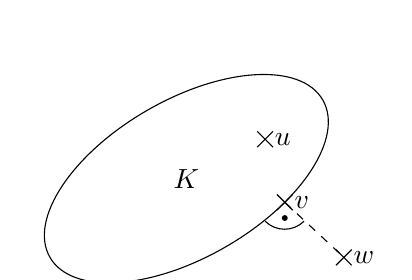
\begin{tikzpicture}
  \draw[rotate=30] (0,0) ellipse (2 and 1);
  \node at (0,0) {$K$};
  \draw (2,-1) node[right]{$w$}  +(-0.1,-0.1) -- +(0.1,0.1) +(0.1,-0.1) -- +(-0.1,0.1);
  \draw (1,0.5) node[right]{$u$}  +(-0.1,-0.1) -- +(0.1,0.1) +(0.1,-0.1) -- +(-0.1,0.1);
  \draw (1.25,-0.3) node[right]{$v$}  +(-0.1,-0.1) -- +(0.1,0.1) +(0.1,-0.1) -- +(-0.1,0.1);
  \draw[dashed] (1.25,-0.3) -- (2,-1);
  \draw (1,-0.54) arc [radius=0.35,start angle=225,delta angle=90];
  \draw[fill] (1.25,-0.5) circle (0.03);
\end{tikzpicture}\hfill{}\hspace*{1mm}\caption{$\norm{v-w}=\inf_{u\in K}\norm{u-w}$}
\end{figure}


If $K$ were compact, then choose minimizing sequence (\foreignlanguage{ngerman}{Minimalfolge}),
i.e.:
\begin{align*}
\norm{u_{i}-w} & \to\inf_{u\in K}\norm{u-w}
\end{align*}
Choose a convergent subsequence $u_{i_{l}}\to v$. Then by continuity:
\begin{align*}
\norm{v-w} & =\lim_{i\to\infty}\norm{u_{i}-w}=\inf_{u\in K}\norm{u-w}
\end{align*}


The main application are closed subspaces $K\subseteq H$.

\begin{figure}[h]
\hspace*{1mm}\hfill{}\begin{tikzpicture}
  \draw (0,0) -- (3,3) node [above right]{$K$};
  \draw (3,-1) node[right]{$w$}  +(-0.1,-0.1) -- +(0.1,0.1) +(0.1,-0.1) -- +(-0.1,0.1);
  \draw (1,1) node[right]{$v$}  +(-0.1,-0.1) -- +(0.1,0.1) +(0.1,-0.1) -- +(-0.1,0.1);
  \draw[dashed] (1,1) -- (3,-1);
  \draw (0.75,0.75) arc [radius=0.35,start angle=225,delta angle=90];
  \draw[fill] (1,0.8) circle (0.03);
\end{tikzpicture}\hfill{}\hspace*{1mm}\caption{$v-w\perp K$}
\end{figure}


In this case $v-w$ will be called orthogonal to $K$ motivating the
name \emph{orthogonal projection}.


\subsection{Theorem \textmd{(Hilbert)\label{sub:Thm-Hilbert}}}

There is a unique $v\in K$ with:
\begin{align*}
\norm{v-w} & =\inf_{u\in K}\norm{u-w}
\end{align*}



\subsubsection*{Proof}

Consider a minimizing sequence $u_{i}$:
\begin{align*}
\norm{u_{i}-w} & \to\inf_{u\in K}\norm{u-w}=:d
\end{align*}
We show that $\left(u_{i}\right)$ is a Cauchy sequence:
\begin{align*}
\norm{u_{i}-u_{j}}^{2} & =\norm{\left(u_{i}-w\right)+\left(w-u_{j}\right)}^{2}=\\
 & \stackrel{\ref{sub:Lem-parallelogram-equality}}{=}2\norm{u_{i}-w}^{2}+2\norm{w-u_{j}}^{2}-\norm{\left(u_{i}-w\right)-\left(w-u_{j}\right)}^{2}=\\
 & =2\norm{u_{i}-w}^{2}+2\norm{w-u_{j}}^{2}-\norm{-2\left(w-\frac{u_{i}+u_{j}}{2}\right)}^{2}=\\
 & =2\left(\underbrace{\norm{u_{i}-w}^{2}}_{\to d^{2}}+\underbrace{\norm{w-u_{j}}^{2}}_{\to d^{2}}-2\norm{\frac{u_{i}+u_{j}}{2}-w}^{2}\right)
\end{align*}
\begin{align*}
\norm{u_{i}-w} & \xrightarrow{i\to\infty}d=\inf_{u\in K}\norm{u-w}\\
\norm{u_{j}-w} & \xrightarrow{j\to\infty}d=\inf_{u\in K}\norm{u-w}
\end{align*}
Since $K$ is convex and $u_{i},u_{j}\in K$, we know:
\begin{align*}
\frac{u_{i}+u_{j}}{2} & \in K
\end{align*}
\begin{align*}
\Rightarrow\quad\norm{\frac{u_{i}+u_{j}}{2}-w} & \ge d
\end{align*}
Thus:
\begin{align*}
\norm{u_{i}-u_{j}}^{2} & \le2\left(\norm{u_{i}-w}^{2}+\norm{w-u_{j}}^{2}-2d^{2}\right)\xrightarrow{i,j\to\infty}2\left(d^{2}+d^{2}-2d^{2}\right)=0
\end{align*}
So there exists a $N\in\mathbb{N}$ such that $\norm{u_{i}-u_{j}}<\varepsilon$
for all $i,j>N$. Therefore $\left(u_{i}\right)$ is a Cauchy sequence.
Since $H$ is complete, we know that $u_{i}\to u$ converges.\\
By continuity follows:
\begin{align*}
\norm{u-w} & =\lim_{i\to\infty}\norm{u_{i}-w}=d
\end{align*}
Uniqueness follows from the fact, that \emph{every} minimizing sequence
converges:\\
Let $u,\tilde{u}$ be both minimizers, then the sequence $\left(u,\tilde{u},u,\tilde{u},\ldots\right)$
is a minimizing sequence. Since it converges, $u=\tilde{u}$.\qqed


\subsection{Corollary}

Let $M\subseteq H$ be a closed subspace of $H$. Then a $w\in H$
can be decomposed uniquely in the form
\begin{align*}
w & =v+x
\end{align*}
with $v\in M$ and $x\in M^{\perp}$. We write $H=M\oplus M^{\perp}$.

\begin{figure}[h]
\hspace*{1mm}\hfill{}\begin{tikzpicture}[arr/.style={decoration={markings,mark=at position 1 with {\arrow[thick]{>}}},postaction={decorate}}]
  \draw (-1,-1) -- (3,3) node [above right]{$M$};
  \draw (4,0) node[right]{$w$}  +(-0.1,-0.1) -- +(0.1,0.1) +(0.1,-0.1) -- +(-0.1,0.1);
  \draw (2,2) +(-0.1,-0.1) -- +(0.1,0.1) +(0.1,-0.1) -- +(-0.1,0.1);
  \draw (0,0) node[below right]{$0$}  +(-0.1,-0.1) -- +(0.1,0.1) +(0.1,-0.1) -- +(-0.1,0.1);
  \draw [arr] (0,0) -- node[above]{$v$} (2,2);
  \draw[arr] (2,2) -- node[right]{$x$} (4,0);
  \draw (1.75,1.75) arc [radius=0.35,start angle=225,delta angle=90];
  \draw[fill] (2,1.8) circle (0.03);
\end{tikzpicture}\hfill{}\hspace*{1mm}\caption{$w=v+x$}
\end{figure}



\subsubsection*{Proof}

Let $v\in M$ be as in Theorem \ref{sub:Thm-Hilbert}.
\begin{align*}
\norm{v-w} & =\inf_{u\in M}\norm{u-w}
\end{align*}
Define $x:=w-v$.
\begin{itemize}
\item $H$ real: For $u\in M$ define $\tilde{u}\left(\tau\right)=v+\tau u$
with $\tau\in\mathbb{R}$.
\begin{align*}
\norm{\tilde{u}-w}^{2} & =\norm x^{2}+2\tau\left\langle u,x\right\rangle +\tau^{2}\norm u^{2}\ge\norm x^{2}\\
0 & \le2\tau\left\langle u,x\right\rangle +\tau^{2}\norm u^{2}=:f\left(\tau\right)
\end{align*}
$f\left(\tau\right)$ has a minimum at $\tau=0$ and so $f'\left(0\right)=0$.
\begin{align*}
f'\left(0\right) & =2\left\langle u,x\right\rangle \\
\Rightarrow\quad2\left\langle u,x\right\rangle  & =0\quad\fall_{u\in M}
\end{align*}
So $x\in M^{\perp}$.
\item $H$ complex: Define $\tilde{u}\left(\tau\right)=v+\tau u$, $\tau=re^{\ii\varphi}\in\mathbb{K}$
with $r\ge0$.
\begin{align*}
\norm{\tilde{u}-w}^{2} & =\norm x^{2}+2\text{Re}\left(re^{-\ii\varphi}\left\langle u,x\right\rangle \right)+r^{2}\norm u^{2}=:f\left(r,\varphi\right)
\end{align*}
This has a minimum at $r=0$.
\begin{align*}
\Rightarrow\quad0 & =\partial_{r}f\left(0,\varphi\right)=2\text{Re}\left(e^{-\ii\varphi}\left\langle u,x\right\rangle \right)\\
\stackrel{\varphi\text{ arbitrary}}{\Rightarrow}\quad\left\langle u,x\right\rangle  & =0
\end{align*}
So $x\in M^{\perp}$.
\end{itemize}
%DATE: Fr 9.11.12

\emph{Uniqueness}: Assume that $w=v_{1}+x_{1}=v_{2}+x_{2}$ where
$v_{1},v_{2}\in M$, $x_{1},x_{2}\in M^{\perp}$.
\begin{align*}
\underbrace{v_{1}-v_{2}}_{\in M} & =\underbrace{x_{2}-x_{1}}_{\in M^{\perp}}\in M\cap M^{\perp}=\left\{ 0\right\} 
\end{align*}
Because from $u\in M\cap M^{\perp}$ follows $\left\langle u,u\right\rangle =0$
and so $u=0$.\qqed

For a Banach space $E$ we have $E,E^{*},E^{**}$ and a natural injection
$\iota:E\hookrightarrow E^{**}$.\\
For a Hilbert space $H$, suppose $u\in H$ and define:
\begin{align*}
\varphi:H & \to\mathbb{K}\\
\varphi\left(v\right) & :=\left\langle u,v\right\rangle 
\end{align*}
$\varphi$ is continuous, because:
\begin{align*}
\abs{\varphi\left(v\right)}=\abs{\left\langle u,v\right\rangle } & \le\norm u\cdot\norm v\le C\norm v
\end{align*}
Now
\begin{align*}
\iota:H & \hookrightarrow H^{*}\\
\iota\left(u\right) & =\varphi
\end{align*}
is a linear mapping, which is injective.


\subsection{Theorem \textmd{(Fréchet-Riesz)}}

For any $\varphi\in H^{*}$ there is a unique $v\in H$ such that
for all $x\in H$:
\begin{align*}
\varphi\left(x\right) & =\left\langle v,x\right\rangle 
\end{align*}
In other words: $\iota:H\to H^{*}$ is a Banach space isomorphism.


\subsubsection*{Proof}

Let $\varphi\in H^{*}$, without loss of generality $\varphi\not=0$.
\begin{align*}
M & :=\ker\varphi\subseteq H
\end{align*}
is a subspace. It is closed by continuity: For $u_{n}\in\ker\varphi$
with $u_{n}\to u$ holds:
\begin{align*}
\varphi\left(u\right) & \stackrel{\text{continuity}}{=}\lim_{n\to\infty}\varphi\left(u_{n}\right)=0
\end{align*}
So $u\in\ker\varphi$.

\begin{figure}[h]
\hspace*{1mm}\hfill{}\begin{tikzpicture}[arr/.style={decoration={markings,mark=at position 1 with {\arrow[thick]{>}}},postaction={decorate}}]
  \draw (-1,-1) -- (3,3) node [above right]{$M$};
  \draw (4,0) node[right]{$u$}  +(-0.1,-0.1) -- +(0.1,0.1) +(0.1,-0.1) -- +(-0.1,0.1);
  \draw (2,2) +(-0.1,-0.1) -- +(0.1,0.1) +(0.1,-0.1) -- +(-0.1,0.1);
  \draw (0,0) node[below right]{$0$}  +(-0.1,-0.1) -- +(0.1,0.1) +(0.1,-0.1) -- +(-0.1,0.1);
  \draw [arr] (0,0) -- node[above]{$v$} (2,2);
  \draw[arr] (2,2) -- node[right]{$x$} (4,0);
  \draw (1.75,1.75) arc [radius=0.35,start angle=225,delta angle=90];
  \draw[fill] (2,1.8) circle (0.03);
\end{tikzpicture}\hfill{}\hspace*{1mm}\caption{$u=v+x$}
\end{figure}

\begin{itemize}
\item $M^{\perp}$ is a one-dimensional subspace of $H$:\\
$M^{\perp}\not=\left\{ 0\right\} $:\\
Since $\varphi\not=0$ there exists a $u\in H$ with $\varphi\left(u\right)\not=0$,
thus $u\not\in M$.\\
Now decompose $u=v+x$, $v\in M$, $x\in M^{\perp}\setminus\left\{ 0\right\} $.\\
$M^{\perp}$ is one-dimensional: Take $u,v\in M^{\perp}$, $u,v\not=0$,
then $\varphi\left(u\right)\not=0$ and $\varphi\left(v\right)\not=0$.
\begin{align*}
\varphi\left(\varphi\left(v\right)u-\varphi\left(u\right)v\right) & =0
\end{align*}
So $\varphi\left(v\right)u-\varphi\left(u\right)v\in M\cap M^{\perp}=\left\{ 0\right\} $.
Thus $\varphi\left(v\right)u-\varphi\left(u\right)v=0$, implying
that $u$ and $v$ are linearly dependent.
\item Choose $u\in M^{\perp}$ with $\varphi\left(u\right)=1$, which is
always possible by rescaling.
\begin{align*}
v & :=\frac{u}{\norm u^{2}}\\
\Rightarrow\quad\varphi\left(v\right) & =\frac{1}{\norm u^{2}}\underbrace{\varphi\left(u\right)}_{=1}=\frac{1}{\norm u^{2}}\\
\left\langle v,v\right\rangle  & =\frac{\left\langle u,u\right\rangle }{\norm u^{4}}=\frac{1}{\norm u^{2}}=\varphi\left(v\right)
\end{align*}

\item This $v$ has the desired properties:\\
For $x\in H$ decompose:
\begin{align*}
x & =\underbrace{m}_{\in M}+\underbrace{\alpha v}_{\in M^{\perp}=\left\langle v\right\rangle }
\end{align*}
\begin{align*}
\Rightarrow\quad\varphi\left(x\right) & =\underbrace{\varphi\left(m\right)}_{=0}+\alpha\varphi\left(v\right)=\alpha\left\langle v,v\right\rangle =\\
 & =\left\langle v,\alpha v\right\rangle =\left\langle v,m+\alpha v\right\rangle =\left\langle v,x\right\rangle 
\end{align*}

\end{itemize}
\qqed


\subsection{Theorem \textmd{(Lax-Milgram)}}

Let $H$ be a Hilbert space and $B:H\times H\to\mathbb{K}$ be a mapping
with the following properties:
\begin{enumerate}[label=\roman*)]
\item $B\left(x,y\right)$ is linear in the second an anti-linear in the
first argument.
\item $\abs{B\left(x,y\right)}\le C\norm x\cdot\norm y$ (continuity)
\item $B$ is symmetric ($\overline{B\left(x,y\right)}=B\left(y,x\right)$)
and positive definite, i.e. $B\left(x,x\right)\ge b\norm x^{2}$ with
$b\in\mathbb{R}_{>0}$.
\item [iii')] $\abs{B\left(x,x\right)}\ge b\norm x^{2}$ with $b\in\mathbb{R}_{>0}$.
\end{enumerate}
Then every $l\in H^{*}$ can be represented uniquely as:
\begin{align*}
l\left(y\right) & =B\left(x,y\right)\qquad\fall_{y\in H}
\end{align*}



\subsubsection*{Proof}

First the easy case iii):\\
We introduce a new scalar product $\left\langle .,.\right\rangle _{B}$
by:
\begin{align*}
\left\langle x,y\right\rangle _{B} & :=B\left(x,y\right)
\end{align*}
Using ii) and iii) one sees that $\norm ._{B}$ is equivalent to $\norm .$,
i.e. there exists a $C\in\mathbb{R}_{>0}$ such that:
\begin{align*}
\frac{1}{C}\norm x & \le\norm x_{B}\le C\norm x
\end{align*}
According to the Fréchet-Riesz theorem, there exists a unique $v\in H$
with
\begin{align*}
\varphi\left(x\right) & =\left\langle v,x\right\rangle _{B}=B\left(v,x\right)
\end{align*}
for all $x\in H$.

More difficult case iii'): Given $x\in H$,
\begin{align*}
B\left(x,.\right):H & \to\mathbb{K}
\end{align*}
is a linear bounded functional according to i) and ii), i.e. $B\left(x,.\right)\in H^{*}$.\\
According to the Fréchet-Riesz theorem there exists a unique $z\in H$
such that $B\left(x,y\right)=\left\langle z,y\right\rangle $ for
all $y\in H$. This yields a mapping:
\begin{align*}
\varphi:H & \to H\\
x & \mapsto z
\end{align*}
\begin{align*}
B\left(x,y\right) & =\left\langle \varphi\left(x\right),y\right\rangle 
\end{align*}

\begin{itemize}
\item $\varphi$ is linear, because both $B$ and $\left\langle .,.\right\rangle $
are anti-linear in their first arguments.
\item $\varphi\left(H\right)\subseteq H$ is closed:
\begin{align}
b\norm x^{2}\stackrel{\text{iii')}}{\le}\abs{B\left(x,x\right)} & =\abs{\left\langle z,x\right\rangle }\le\norm z\cdot\norm x\nonumber \\
b\norm x & \le\norm z\label{eq:bx<z}
\end{align}
Let $z_{n}\in\varphi\left(H\right)$ be a sequence with $z_{n}\to z\in H$.
Choose $x_{n}$ such that $\varphi\left(x_{n}\right)=z_{n}$, i.e.
$B\left(x_{n},y\right)=\left\langle z_{n},y\right\rangle $ for all
$y\in H$.\\
Due to the anti-linearity in the first argument follows that:
\begin{align*}
B\left(x_{n}-x_{m},y\right) & =\left\langle z_{n}-z_{m},y\right\rangle 
\end{align*}
\eqref{eq:bx<z} yields that $\norm{x_{n}-x_{m}}\le\norm{z_{n}-z_{m}}$.\\
Hence $\left(x_{n}\right)$ is a Cauchy sequence and so $x_{n}\to x\in H$
converges. Since $B$ is continuous according to ii), we get:
\begin{align*}
\underbrace{B\left(x_{n},y\right)}_{\to B\left(x,y\right)} & =\underbrace{\left\langle z_{n},y\right\rangle }_{\to\left\langle z,y\right\rangle }
\end{align*}
This gives:
\begin{align*}
B\left(x,y\right) & =\left\langle z,y\right\rangle \\
\varphi\left(x\right) & =z
\end{align*}
Thus $z$ is in $\varphi\left(H\right)$.
\item $\varphi\left(H\right)=H$: Otherwise there would be a vector $y\in\varphi\left(H\right)^{\perp}\setminus\left\{ 0\right\} $
and thus for all $x\in H$ holds.
\begin{align*}
B\left(x,y\right) & =\left\langle \varphi\left(x\right),y\right\rangle =0
\end{align*}
In particular for $x=y$ this gives:
\begin{align*}
0 & =\abs{B\left(y,y\right)}\ge b\norm y^{2}\\
\Rightarrow\quad y & =0
\end{align*}
This is a contradiction and so $\varphi\left(H\right)=H$.
\item $\varphi$ is injective: Suppose there are $x,\, x'\in H$ with $\varphi\left(x\right)=\varphi\left(x'\right)$.
Then follows:
\begin{align*}
B\left(x-x',y\right) & =\big<\underbrace{\varphi\left(x\right)-\varphi\left(x'\right)}_{=0},y\big>=0
\end{align*}
Choose $y=x-x'$ so we get:
\begin{align*}
B\left(x-x',x-x'\right) & =0
\end{align*}
Since $B$ is positive definite, it follows $x=x'$.
\item Let $l\in H^{*}$. According to Fréchet-Riesz there exists a unique
$z\in H$ with $l\left(y\right)=\left\langle z,y\right\rangle $ for
all $y\in H$ and we have
\begin{align*}
\left\langle z,y\right\rangle  & =B\left(x,y\right)
\end{align*}
for $x=\varphi^{-1}\left(z\right)$. So $l\left(y\right)=B\left(x,y\right)$.
\end{itemize}
\qqed


\subsection{Corollary}

Every Hilbert space is reflexive.


\subsubsection*{Proof}

Recall $\iota:H\hookrightarrow H^{**}$. $H$ is \emph{reflexive}
if and only if $\iota$ is surjective, i.e. a Banach space isomorphism.
\begin{align*}
\tilde{\iota}:H & \to H^{*}\\
\left(\tilde{\iota}\left(u\right)\right)\left(v\right) & =\left\langle u,v\right\rangle 
\end{align*}
is bijective by Fréchet-Riesz. This holds also for $\overline{\iota}:H^{*}\to H^{**}$.
\begin{align*}
H\stackrel{\tilde{\iota}}{\to}H^{*}\stackrel{\overline{\iota}}{\to}H^{**}
\end{align*}
So $\iota=\overline{\iota}\circ\tilde{\iota}$ is bijective as composition
of bijective maps.\qqed


\section{Orthonormal Bases in Separable Hilbert Spaces}


\subsection{Example}

\begin{align*}
\ell_{2} & =\left\{ \left(a_{n}\right)_{n\in\mathbb{N}}\bigg|\sum_{n\in\mathbb{N}}\abs{a_{n}}^{2}<\infty\right\} 
\end{align*}
with the scalar product
\begin{align*}
\left\langle \left(a_{n}\right),\left(b_{n}\right)\right\rangle  & :=\sum_{n}\overline{a}_{n}b_{n}
\end{align*}
is a Hilbert space.

Idea: Let $H$ be an abstract Hilbert space. Choose an ``orthonormal
basis'' $\left(e_{i}\right)$.
\begin{align*}
H\ni u & =\sum_{i=1}^{\infty}\lambda_{i}e_{i}\\
v & =\sum_{i=1}^{\infty}\nu_{i}e_{i}
\end{align*}
\begin{align*}
\left\langle u,v\right\rangle  & =\sum_{i,j=1}^{\infty}\left\langle \lambda_{i}e_{i},\nu_{j}e_{j}\right\rangle =\sum_{i,j=1}^{\infty}\overline{\lambda_{i}}\nu_{j}\delta_{ij}=\sum_{i}\overline{\lambda_{i}}\nu_{i}
\end{align*}



\subsection{Definition \textmd{(orthonormal system, Hilbert space basis, cardinality)}}

A system $\left(e_{i}\right)_{i\in J}$ is an \emph{orthonormal system},
if $\left\langle e_{i},e_{j}\right\rangle =\delta_{ij}$. The algebraic
span is the vector space of \emph{finite} linear combinations:
\begin{align*}
\left\langle \left(e_{i}\right)\right\rangle  & =\left\{ \sum_{i=1}^{N}\lambda_{i}e_{i}\big|N\in\mathbb{N},\lambda_{i}\in\mathbb{K}\right\} 
\end{align*}
This is a subspace of $H$. Now the subspace $\overline{\left\langle \left(e_{i}\right)\right\rangle }\subseteq H$
is called \emph{Hilbert space span} (\foreignlanguage{ngerman}{Hilbertraumerzeugnis}).

An orthonormal system $\left(e_{i}\right)$ is called a \emph{orthonormal
Hilbert space basis} if $\overline{\left\langle \left(e_{i}\right)\right\rangle }=H$.

Two sets $A$ and $B$ have the same cardinality if there exists an
bijective map $\varphi:A\to B$.


\subsubsection*{Theorem \textmd{(Bernstein-Schröder)}}

$A$ and $B$ have the same cardinality if and only if there exists
an injective map from $A$ to $B$ and an injective map from $B\to A$.


\subsubsection*{(no proof)}

\clearpage{}

%DATE: Do 15.11.12

A typical application of the Lax-Milgram theorem is for $x\in\mathbb{R}^{n}$,
given real-valued functions $V\left(x\right)\!,\, f\left(x\right)$
and looking for $u\left(x\right)$ that solves:
\begin{align*}
-\Delta u\left(x\right)+V\left(x\right)u\left(x\right) & =f\left(x\right)
\end{align*}
Question: Is there a solution which ``decays at infinity''?
\begin{enumerate}
\item Weak formulation:\\
Suppose we have a solution $u\in\mathcal{C}^{2}\left(\mathbb{R}^{n}\right)$
\begin{align*}
-\Delta u+Vu-f & =0
\end{align*}
Let $\eta\in\mathcal{C}_{0}^{\infty}\left(\mathbb{R}^{n}\right)$
be a test function.
\begin{align*}
0 & =\int_{\mathbb{R}^{n}}\left(-\Delta u+Vu-f\right)\eta\dd^{n}x\sr ={\text{integration}}{\text{by parts}}\underbrace{\int_{\mathbb{R}^{n}}\left(\left\langle \nabla u,\nabla\eta\right\rangle +Vu\eta\right)\dd^{n}x}_{=:B\left(u,\eta\right)}-\underbrace{\int_{\mathbb{R}^{n}}f\eta\dd^{n}x}_{=l\left(\eta\right)}
\end{align*}
So for all $\eta\in\mathcal{C}_{0}^{\infty}\left(\mathbb{R}^{n}\right)$
holds:
\begin{align*}
B\left(u,\eta\right) & =l\left(\eta\right)
\end{align*}
\textbf{Definition:} $u$ is a \emph{weak solution} of the equation
$-\Delta u+Vu=f$ if for all $\eta\in\mathcal{C}_{0}^{\infty}\left(\mathbb{R}^{n}\right)$
holds:
\begin{align*}
B\left(u,\eta\right) & =l\left(\eta\right)
\end{align*}

\item Choose the correct Hilbert space. The first idea is $L^{2}\left(\mathbb{R}^{n}\right)$
with the scalar product:
\begin{align*}
\left\langle u,v\right\rangle  & =\int_{\mathbb{R}^{n}}uv\dd^{n}x
\end{align*}
\begin{align*}
u_{n}\left(x\right) & :=e^{-\abs x^{2}}\sin\left(nx_{1}\right)
\end{align*}
Then for all $n\in\mathbb{N}$ holds:
\begin{align*}
\norm{u_{n}}_{L^{2}} & \le C
\end{align*}
But $B\left(u_{n},u_{n}\right)\xrightarrow{n\to\infty}\infty$ diverges.
Thus $B$ is \emph{not} continuous.\\
Better choose instead:
\begin{align*}
\left\langle u,v\right\rangle  & =\int_{\mathbb{R}^{n}}\left(uv+\left\langle \nabla u,\nabla v\right\rangle \right)\dd^{n}x
\end{align*}
The corresponding Hilbert space $H^{1,2}\left(\mathbb{R}^{n}\right)$
is a Sobolev space.
\begin{align*}
L^{2}\left(\mathbb{R}^{3}\right) & \supseteq H^{1,2}\left(\mathbb{R}^{3}\right)\ni u
\end{align*}
Assume for simplicity that $0<\varepsilon\le V\le C<\infty$, then
we get:
\begin{align*}
B\left(u,u\right) & =\int_{\mathbb{R}^{n}}\left(\abs{\nabla u}^{2}+Vu^{2}\right)\dd^{n}x\le\int_{\mathbb{R}^{n}}\left(\abs{\nabla u}^{2}+Cu^{2}\right)\dd^{n}x\le\left(1+C\right)\norm u_{H^{1,2}}^{2}
\end{align*}
\begin{align*}
\abs{B\left(u,u\right)} & \ge\int\left(\abs{\nabla u}^{2}+\varepsilon u^{2}\right)\ge\min\left\{ 1,\varepsilon\right\} \norm u_{H^{1,2}}^{2}
\end{align*}
Thus the Lax-Milgram theorem applies and yields a unique weak solution
and then a regularity theorem says that $u$ is smooth.
\end{enumerate}
Consider a matrix equation
\begin{align*}
Au & =f
\end{align*}
with $A\in\text{Symm}\left(\mathbb{R}^{n}\right)$ and $f\in\mathbb{R}^{n}$.\\
For a general existence and uniqueness result one needs that $A$
is invertible or equivalently:
\begin{align*}
\fall_{u\in\mathbb{R}^{n}\setminus\left\{ 0\right\} }:\ Au & \not=0
\end{align*}
This follows from the condition:
\begin{align*}
\fall_{u\in\mathbb{R}^{n}\setminus\left\{ 0\right\} }:\ \underbrace{\left\langle u,Au\right\rangle }_{=B\left(u,u\right)} & \not=0
\end{align*}
In finite dimension this is equivalent to:
\begin{align*}
\fall_{u\in\mathbb{R}^{n}}:\ \abs{B\left(u,u\right)} & >b\norm u^{2}
\end{align*}


$\left(e_{i}\right)_{i\in I}$ is an orthonormal Hilbert space basis
of $H$ if
\begin{align*}
\left\langle e_{i},e_{j}\right\rangle  & =\delta_{ij}
\end{align*}
and:
\begin{align*}
\overline{\left\langle e_{i}\right\rangle } & =H
\end{align*}



\subsection{Theorem}

Let $\left(e_{i}\right)_{i\in\mathbb{N}}$ be an orthonormal system.
Then the mapping
\begin{align*}
\ell_{2} & \to\overline{\left\langle e_{i}\right\rangle }\stackrel{\text{closed}}{\subseteq}H\\
\left(\lambda_{i}\right) & \mapsto\sum_{i\in\mathbb{N}}\lambda_{i}e_{i}
\end{align*}
is a Hilbert space isomorphism.


\subsubsection{Proof}

The mapping is well-defined and isometric:\\
For $\left(\lambda_{i}\right)\in\ell_{2}$, i.e. $\sum_{i\in\mathbb{N}}\abs{\lambda_{i}}^{2}<\infty$
we construct:
\begin{align*}
u_{N} & :=\sum_{i=1}^{N}\lambda_{i}e_{i}\in H
\end{align*}
Without loss of generality take $M<N$, then follows:
\begin{align*}
\norm{u_{N}-u_{M}}^{2} & =\norm{\sum_{i=M}^{N}\lambda_{i}e_{i}}^{2}=\left\langle \sum_{i=M}^{N}\lambda_{i}e_{i},\sum_{i=M}^{N}\lambda_{i}e_{i}\right\rangle =\sum_{i,j=M}^{N}\overline{\lambda_{i}}\lambda_{j}\underbrace{\left\langle e_{i},e_{j}\right\rangle }_{=\delta_{ij}}=\sum_{i=M}^{N}\abs{\lambda_{i}}^{2}
\end{align*}
Thus $u_{N}$ is a Cauchy sequence and converges since $\overline{\left\langle e_{i}\right\rangle }$
is complete as a closed subset of a complete space.
\begin{align*}
u & :=\lim_{N\to\infty}u_{N}=\sum_{i=1}^{N}\lambda_{i}e_{i}
\end{align*}
\begin{align*}
\norm u^{2} & =\lim_{N\to\infty}\norm{u_{N}}^{2}=\lim_{N\to\infty}\sum_{i=1}^{N}\abs{\lambda_{i}}^{2}=\norm{\left(\lambda_{i}\right)}_{\ell_{2}}
\end{align*}
The mapping is also surjective:\\
Let $u\in\overline{\left\langle e_{i}\right\rangle }$ and $\varepsilon>0$.
So there exists a $v=\sum_{i=1}^{N}\lambda_{i}e_{i}\in\left\langle e_{i}\right\rangle $
with $\norm{v-u}<\varepsilon$.\\
In other words there exists a finite $J\subseteq\mathbb{N}$ such
that $d\left(\left\langle \left(e_{i}\right)_{i\in J}\right\rangle ,u\right)<\varepsilon$.
The vector which minimizes this distance is the orthogonal projection
of $u$ on $\left\langle \left(e_{i}\right)_{i\in J}\right\rangle $
since this is a finite-dimensional subspace, which is automatically
closed.
\begin{align*}
u_{J} & =\sum_{i\in J}e_{i}\left\langle e_{i},u\right\rangle 
\end{align*}
Choose an increasing sequence $J_{1}\subsetneq J_{2}\subsetneq\ldots$
of finite sets such that:
\begin{align*}
\norm{u_{J_{k}}-u} & \to0 & \Rightarrow\quad u_{J_{k}} & \to u
\end{align*}
Thus $u_{J_{k}}$ is bounded by a $C\in\mathbb{R}_{>0}$.
\begin{align*}
u_{J_{k}} & =\sum_{i\in J_{k}}e_{i}\underbrace{\left\langle e_{i},u\right\rangle }_{=\lambda_{i}}\\
C>\norm{u_{J_{k}}} & =\sum_{i\in J_{k}}\abs{\lambda_{i}}^{2}
\end{align*}
This gives:
\begin{align*}
\sum_{i\in\mathbb{N}}\abs{\lambda_{i}}^{2} & <\infty
\end{align*}
And so we get:
\begin{align*}
u & =\sum_{i\in\mathbb{N}}\lambda_{i}e_{i}
\end{align*}
\qqed


\subsection{Theorem \textmd{(Existence of Hilbert space basis)}}

In every Hilbert space $H$ exists an orthonormal Hilbert space basis.


\subsubsection*{Proof}

Consider $\left(u_{i}\right)_{i\in I}$ with $I=H$ and $u_{h}=h$
for all $h\in H$. $\left(u_{i}\right)_{i\in I}$ is obviously a generating
system of $H$. On the set
\begin{align*}
X & :=\left\{ \tilde{I}\subseteq I\big|\left(u_{i}\right)_{i\in\tilde{I}}\text{ is an orthonormal system}\right\} 
\end{align*}
defines „$\subseteq$“ a partial ordering.\\
Let $U\subseteq X$ be a totally ordered subset and define:
\begin{align*}
I_{U} & :=\bigcup_{\tilde{I}\in U}\tilde{I}\subseteq I
\end{align*}
$I_{U}$ is an upper bound of $U$ in $X$ if $I_{U}\in X$. Assume
$\left(u_{i}\right)_{i\in I_{U}}$ would not be orthonormal. Then
there would exist $j,k\in I_{U}$ with $\left\langle u_{j},u_{k}\right\rangle \not=\delta_{jk}$.\\
For $j=k$ would hold $\left\langle u_{j},u_{j}\right\rangle \not=1$,
but $j$ lies in $\tilde{I}\in U\subseteq X$ and therefor has to
hold$\left\langle u_{j},u_{j}\right\rangle =1$.\\
 For $j\not=k$ we would get $\left\langle u_{j},u_{k}\right\rangle \not=0$.
But $j$ lies in $\tilde{I}_{j}\in U$ and $k$ in $\tilde{I}_{k}\subseteq U$
and $U$ is totally ordered, i.e. either holds $\tilde{I}_{j}\subseteq\tilde{I}_{k}$
or $\tilde{I}_{k}\subseteq\tilde{I}_{j}$.\\
Without loss of generality assume $\tilde{I}_{j}\subseteq\tilde{I}_{k}$
(otherwise exchange $j$ and $k$). Then $j,k\in\tilde{I}_{k}\in U\subseteq X$
and hence $\left(u_{i}\right)_{i\in\tilde{I}_{j}}$ is an orthonormal
system in contradiction to $\left\langle u_{j},u_{k}\right\rangle \not=0$.
Therefore holds $I_{U}\in X$ and thus $I_{U}$ is an upper bound
of $U$.\\
Using Zorn's lemma we get a maximal element $I_{\text{max}}$ in $X$.
Because $\left(u_{i}\right)_{i\in I_{\text{max}}}$ is an orthonormal
system and thus especially linearly independent, it suffices to show
that this is an generating system of $H$.\\
Assume there exists a $i_{0}\in I$ with $u_{i_{0}}\not\in K:=\overline{\left\langle \left(u_{i}\right)_{i\in I_{\text{max}}}\right\rangle _{\text{alg.}}}$.
Since $K\subseteq H$ is closed and convex, there is an unique projection
$v$ of $u_{i_{0}}$ on $K$ and thus $h:=u_{i_{0}}-v\in K^{\perp}$.
It holds $h=u_{h}$ with $h\in H=I$.\\
Because $I_{\text{max}}$ is maximal, holds then $I_{\text{max}}\cup\left\{ h\right\} \not\in X$
and hence there is a $j\in I_{\text{max}}$ with$\left\langle h,u_{j}\right\rangle \not=0$,
because $h=j$ cannot hold due to $h\not\in I_{\text{max}}$. This
is a contradiction to $h\in K^{\perp}$ and thus holds $K=H$.\\
Therefore $\left(u_{i}\right)_{i\in I_{\text{max}}}$ is an orthonormal
Hilbert space basis of $H$.\qqed


\subsection{Theorem}

Let $H$ be a Hilbert space.
\begin{enumerate}[label=\roman*)]
\item For any $v\in H$ and for any orthonormal system $\left\{ e_{j}\big|j\in J\right\} $,
the set of elements $j\in J$ for which $\left\langle e_{j},v\right\rangle =0$
is finite or countable.
\item Any two Hilbert space bases of $H$ have the same cardinality (\foreignlanguage{ngerman}{Mächtigkeit}).
\end{enumerate}

\subsubsection*{Proof}
\begin{enumerate}[label=\roman*)]
\item Consider $v\in J$. First we show that every $n\in\mathbb{N}$, the
set $J_{n}:=\left\{ j\in J\big|\left\langle e_{j},v\right\rangle >\frac{1}{n}\right\} $
is finite. Indeed, by Bessel’s inequality, for every finite number
of elements $e_{j_{1}},\ldots,e_{j_{N}}$ of the given orthonormal
system, we have:
\begin{align*}
\sum_{k=1}^{N}\abs{\left\langle e_{j_{k}},v\right\rangle }^{2} & \le\norm v^{2}
\end{align*}
Now suppose that for some $n\in\mathbb{N}$, the set $J_{n}$ were
not finite. Then for any $N\in\mathbb{N}$ we could find elements
$e_{j_{1}},\ldots,e_{j_{N}}$ such that $\left\langle e_{j_{k}},v\right\rangle >\frac{1}{n}$
for all $k\in\left\{ 1,\ldots,N\right\} $. Hence, for these elements
holds:
\begin{align*}
\sum_{k=1}^{N}\abs{\left\langle e_{j_{k}},v\right\rangle }^{2} & >N\cdot\frac{1}{n}
\end{align*}
Clearly these becomes larger than $\norm v$ if we make $N$ sufficiently
large. Hence all the sets $J_{n}$ must be finite. But then, we see
that the set
\begin{align*}
\left\{ j\in J\big|\left\langle e_{j},v\right\rangle \not=0\right\}  & =\bigcup_{n\in\mathbb{N}}J_{n}
\end{align*}
is a countable union of finite sets, and as such can be at most countable.\qqed[\roman{enumi})]
\item If $H$ has is finite-dimensional, every Hilbert basis is a Hamel
basis of $H$ and thus the claim follows from linear algebra.\\
If $H$ is infinite-dimensional, let $\left(e_{i}\right)_{i\in I}$
and $\left(b_{j}\right)_{j\in J}$ be two Hilbert bases of $H$. ($I$
and $J$ have infinitely many elements.)\\
For $x\in H=\overline{\left\langle \left(e_{i}\right)_{i\in I}\right\rangle }=\overline{\left\langle \left(b_{j}\right)_{j\in J}\right\rangle }$
define:
\begin{align*}
B_{x} & :=\left\{ j\in J\big|\left\langle x,b_{j}\right\rangle \not=0\right\} 
\end{align*}
By i), the set $B_{x}$ is at most countable for any $x\in H$. Next,
let $j\in J$ be given. Since $\overline{\left\langle \left(e_{i}\right)_{i\in I}\right\rangle }=H$,
we must have $\left\langle b_{j},e_{i}\right\rangle \not=0$ for some
$i\in I$. Otherwise, $b_{j}\in\overline{\left\langle \left(e_{i}\right)_{i\in I}\right\rangle }^{\perp}=\left\{ 0\right\} $,
which is not possible since $b_{j}\not=0$. Therefore, we have $j\in B_{e_{i}}$
for some $i\in I$, and since $j\in J$ was arbitrary, it follows
that $J\subseteq\bigcup_{i\in I}B_{e_{i}}\subseteq I\times\mathbb{N}$.
Here the second inclusion uses that all the sets $B_{e_{j}}$ are
at most countable. It follows:
\begin{align*}
\abs J & \le\abs I\cdot\abs{\mathbb{N}}=\abs I
\end{align*}
If we exchange the roles of $I$ and $J$ above, we also obtain $\abs I\le\abs J$.
By the Schröder-Bernstein theorem, we can combine both estimates to
obtain that $\abs I=\abs J$.\qqed[\roman{enumi})]
\end{enumerate}
\qqed


\subsection{Theorem}

If $H$ is separable, then there exists a countable orthonormal Hilbert
space basis $\left(e_{i}\right)_{i\in\mathbb{N}}$.\\
Thus $H$ is Hilbert space isomorphic to $\ell_{2}$.


\subsubsection{Proof}

Since $H$ is separable, there is a countable dense subset $\left(x_{i}\right)_{i\in\mathbb{N}}$.
\begin{enumerate}
\item Arrange that the $x_{i}$ are linearly independent:\\
Start with $n=1$ and $k=1$ set:
\begin{align*}
y_{1} & =x_{1}
\end{align*}
If the $y_{1},\ldots,y_{n-1},x_{k}$ are linearly independent, we
set $y_{n}=x_{k}$ and increase $n$ and $k$ by one.\\
If the $y_{1},\ldots,y_{n-1},x_{k}$ are linearly dependent, we only
increase $k$ by one.\\
Then the $y_{i}$ are linearly independent and $\left\langle \left(y_{i}\right)\right\rangle =\left\langle \left(x_{i}\right)\right\rangle $.
\item Gram-Schmidt procedure for orthonormalization:
\begin{align*}
e_{1} & :=y_{1}\\
e_{2} & :=\frac{y_{2}-e_{1}\left\langle u_{1},y_{2}\right\rangle }{\norm{y_{2}-e_{1}\left\langle u_{1},y_{2}\right\rangle }}\\
e_{n} & :=\frac{y_{n}-\text{Pr}_{\left\langle e_{1},\ldots,e_{n-1}\right\rangle }y_{n}}{\norm{y_{n}-\text{Pr}_{\left\langle e_{1},\ldots,e_{n-1}\right\rangle }y_{n}}}
\end{align*}
Since the $y_{i}$ are linearly independent, $y_{n}-\text{Pr}_{\left\langle e_{1},\ldots,e_{n-1}\right\rangle }y_{n}$
is never zero.\\
Then by construction the $e_{i}$ are orthonormal and $\left\langle e_{i}\right\rangle =\left\langle x_{i}\right\rangle \subseteq H$
is dense and so $\left(e_{i}\right)_{i\in\mathbb{N}}$ is a Hilbert
space basis.\qqed
\end{enumerate}

\section{Weak Compactness of the Closed Unit Ball}

For a Banach space $E$ \emph{weak convergence} for $\left(u_{i}\right)_{i\in\mathbb{N}}$
with $u_{i}\in E$ means:
\begin{align*}
u_{n} & \rightharpoondown u & \Leftrightarrow\quad\fall_{\varphi\in E^{*}}:\varphi\left(u_{n}\right) & \to\varphi\left(u\right)
\end{align*}
In Hilbert spaces, we can identify $H^{*}$ with $H$ via the Fréchet-Riesz
theorem.


\subsection{Definition \textmd{(weak (sequential) compactness)}}

$x_{n}\rightharpoondown x$ \emph{converges weakly} if $\left\langle y,x_{n}\right\rangle \to\left\langle y,x\right\rangle $
converges for all $y\in H$.

Weak compactness is for us by definition the same as \emph{weak sequential
compactness} (\foreignlanguage{ngerman}{schwache Folgenkompaktheit}):\\
$K\subseteq H$ is \emph{weakly compact} if every sequence $\left(x_{n}\right)$
with $x_{n}\in K$ has a weakly convergent subsequence.


\subsection{Proposition}

Let $H$ be \emph{separable} and infinite-dimensional and let $\left(e_{i}\right)_{i\in\mathbb{N}}$
be an orthonormal Hilbert space basis.

Then $e_{n}\rightharpoondown0$ converges weakly.


\subsubsection*{Proof}

Take $y\in H$ and expand it in the basis:
\begin{align*}
y & =\sum_{i=1}^{\infty}y_{i}e_{i}\\
y_{i} & =\left\langle e_{i},y\right\rangle 
\end{align*}
We know $\left(y_{i}\right)_{i\in\mathbb{N}}\in\ell_{2}$ and in particular
$y_{i}\xrightarrow{i\to\infty}0$, since the elements of an absolutely
convergent series converge to zero. Therefore holds:
\begin{align*}
\left\langle y,e_{n}\right\rangle  & =\overline{y_{n}}\xrightarrow{n\to\infty}0
\end{align*}
Thus $e_{n}\rightharpoondown0$ converges weakly.\qqed


\subsection{Theorem \textmd{(Weak Compactness of the Closed Unit Ball)}}

If $H$ is \emph{separable}, then the closed unit ball $\overline{B_{1}\left(0\right)}=\left\{ u\big|\norm u\le1\right\} $
is weakly compact.


\subsubsection{Proof}

Let $\left(u_{l}\right)$ be a sequence with $u_{l}\in\overline{B_{1}\left(0\right)}$.
Choose an orthonormal Hilbert space basis $\left(e_{n}\right)_{n\in\mathbb{N}}$.
\begin{align*}
u_{l} & =\sum_{n=1}^{\infty}u_{ln}e_{n} & u_{ln} & =\left\langle e_{n},u_{l}\right\rangle  & \left(u_{l,n}\right)_{n\in\mathbb{N}} & \in\ell_{2}
\end{align*}
\begin{align*}
\abs{u_{ln}} & =\abs{\left\langle e_{n},u_{l}\right\rangle }\le\underbrace{\norm{e_{n}}}_{=1}\cdot\norm{u_{l}}\le1
\end{align*}
For $n=1$: $\left(u_{l,1}\right)_{l\in\mathbb{N}}$ is a bounded
sequence of complex or real numbers. Therefore there exists a convergent
subsequence of $u_{l}$, which we denote by $u_{l}^{\left(1\right)}\in H$.
Then follows:
\begin{align*}
u_{l,1}^{\left(1\right)} & =\left\langle e_{1},u_{l}^{\left(1\right)}\right\rangle \xrightarrow{l\to\infty}v_{1}
\end{align*}
For $n=2$: Next we choose a subsequence $u_{l}^{\left(2\right)}$
of $u_{l}^{\left(1\right)}$ such that:
\begin{align*}
\left\langle e_{2},u_{l}^{\left(2\right)}\right\rangle  & \xrightarrow{l\to\infty}v_{2}
\end{align*}
Proceed inductively to obtain:
\begin{align*}
\left\langle e_{n},u_{l}^{\left(n\right)}\right\rangle  & \to v_{n}
\end{align*}
Then $w_{l}=u_{l}^{\left(l\right)}\in\overline{B_{1}\left(0\right)}$
for a sequence $\left(w_{l}\right)$ in $\overline{B_{1}\left(0\right)}$.
\begin{description}
\item [{Claim:}] $w_{l}\stackrel{l\to\infty}{\rightharpoondown}v:=\sum_{n}v_{n}e_{n}$
\item [{Proof:}] We proceed as follows:
\begin{align*}
v_{n}=\lim_{l\to\infty}\left\langle e_{n},u_{l}^{\left(n\right)}\right\rangle  & =\lim_{l\to\infty}\left\langle e_{n},u_{l}^{\left(l\right)}\right\rangle =\lim_{l\to\infty}\left\langle e_{n},w_{l}\right\rangle 
\end{align*}
This is because $u_{l}^{\left(l\right)}=u_{l'}^{\left(n\right)}$
for $l'\ge l$.

\begin{enumerate}
\item $\left(v_{n}\right)\in\ell_{2}$:
\begin{align*}
\sum_{n=1}^{N}\abs{v_{n}}^{2} & =\sum_{n=1}^{N}\abs{\lim_{l\to\infty}\left\langle e_{n},w_{l}\right\rangle }^{2}\stackrel{\text{finite sum}}{=}\lim_{l\to\infty}\underbrace{\sum_{n=1}^{N}\abs{\left\langle e_{n},w_{l}\right\rangle }^{2}}_{\sr{\le}{\text{Bessel's}}{\text{inequality}}\norm{w_{l}}^{2}\le1}
\end{align*}
So we get for all $N\in\mathbb{N}$:
\begin{align*}
\sum_{n=1}^{N}\abs{v_{n}}^{2} & \le1
\end{align*}
And thus $\left(v_{n}\right)\in\ell_{2}$ and $v:=\sum_{n=1}^{\infty}v_{n}e_{n}$
is well-defined and has $\norm v\le1$.
\item $w_{l}\rightharpoondown v$, i.e. $\left\langle y,w_{l}-v\right\rangle \xrightarrow{l\to\infty}0$
for all $y\in H$:
\begin{align*}
y & =\sum_{n=1}^{\infty}y_{n}e_{n}
\end{align*}
\begin{align*}
y_{n} & =\left\langle e_{n},y\right\rangle \\
y_{<} & :=\sum_{n\le N}y_{n}e_{n}\\
y_{>} & :=\sum_{n>N}y_{n}e_{n}\\
\norm y^{2} & =\norm{y_{<}}^{2}+\norm{y_{>}}^{2}
\end{align*}
\begin{align*}
\left\langle y,w_{l}-v\right\rangle  & =\sum_{n=1}^{\infty}y_{n}\left\langle e_{n},w_{l}-v\right\rangle 
\end{align*}
Choose $N\in\mathbb{N}$ so large that
\begin{align*}
\norm{y_{>}}=\left(\sum_{n>N}\abs{y_{n}}^{2}\right)^{\frac{1}{2}} & <\frac{\varepsilon}{4}
\end{align*}
to get:
\begin{align*}
\abs{\left\langle y,w_{l}-v\right\rangle } & \le\abs{\left\langle y_{<},w_{l}-v\right\rangle }+\abs{\left\langle y_{>},w_{l}-v\right\rangle }\le\\
 & \le\sum_{n=1}^{N}\abs{y_{n}}\abs{\left\langle e_{n},w_{l}-v\right\rangle }+\underbrace{\norm{y_{>}}}_{<\frac{\varepsilon}{4}}\cdot\underbrace{\norm{w_{l}-v}}_{\le2}<\sum_{n=1}^{N}\abs{y_{n}}\abs{\left\langle e_{n},w_{l}-v\right\rangle }+\frac{\varepsilon}{2}
\end{align*}
We know $\abs{\left\langle e_{n},w_{l}-v\right\rangle }\xrightarrow{l\to\infty}0$
for each $n$. So we can choose $\abs{\left\langle e_{n},w_{l}-v\right\rangle }\le\frac{\varepsilon}{2}$
for $n\le N$ and for all $l>L\left(\varepsilon\right)$ for a sufficiently
large $L\left(\varepsilon\right)$ and therefore:
\begin{align*}
\abs{\left\langle y,w_{l}-v\right\rangle } & \le\varepsilon\qquad\fall_{l>L\left(\varepsilon\right)}
\end{align*}
Therefore $\left\langle y,w_{l}\right\rangle \to\left\langle y,v\right\rangle $
converges, which means $w_{l}\rightharpoondown v$.\qqed[Claim]
\end{enumerate}
\end{description}
\qqed

%DATE: Fr 16.11.12

The corresponding statement in Banach spaces is the \emph{Banach-Alaoglu
theorem}:

Banach proved it in 1932 for separable Banach spaces using diagonal
sequences.

Alaoglu proved it in 1938 for any Banach space. The proof is based
on Tychonov's theorem.

We have $E$, $E^{*}$, $E^{**}$ and an injection $\iota:E\to E^{**}$.


\subsubsection*{Theorem \textmd{(Banach-Alaoglu)}}

The closed unit ball in $E^{*}$ is \emph{weak-$*$-sequentially compact}.

I.e. in simple terms:

If $\varphi_{n}\in\overline{B_{1}\left(0\right)}\subseteq E^{*}$,
then there exists a subsequence $\varphi_{n_{l}}$ such that $\varphi_{n_{l}}\left(u\right)$
converges for all $u\in E$.

Application: Consider
\begin{align*}
E & =C^{0}\left(\mathbb{R}^{n}\right)
\end{align*}
with the sup-norm:
\begin{align*}
\norm f & =\sup_{x\in\mathbb{R}^{n}}\abs{f\left(x\right)}
\end{align*}
\begin{align*}
E^{*} & =\left\{ \text{regular Borel measures}\right\} 
\end{align*}
Suppose $\mu_{n}$ is a sequence of measures with $\norm{\mu_{n}}\le C$
for all $n\in\mathbb{N}$. Then there exists a measure $\mu$ such
that $\mu_{n_{l}}\to\mu$ converges as a measure.


\chapter{Operators on Hilbert spaces}

\setcounter{subsection}{0}

Let $H$ be a Hilbert space.
\begin{align*}
L\left(H\right) & :=L\left(H,H\right)
\end{align*}
is the Banach space of bounded linear operators. (An linear map on
an infinite dimensional space is usually called \emph{linear operator}.)
For $A\in L\left(H\right)$ define the norm:
\begin{align*}
\opnorm A & :=\sup_{\norm u=1}\norm{Au}
\end{align*}



\subsection{Example}

$H=L^{2}\left(\mathbb{R},\dd x\right)$ with the Lebesgue measure
$\dd x$.
\begin{align*}
\left\langle f,g\right\rangle  & =\int_{\mathbb{R}}\overline{f}g\dd x
\end{align*}
\begin{align*}
A & :=\frac{\dd}{\dd x}
\end{align*}
We would like to introduce this as an operator on $H$.\\
The inequality $\norm{Au}\le C\norm u$ is violated even for $u\in C_{0}^{\infty}\left(\mathbb{R}\right)$
for any constant $C\in\mathbb{R}$.\\
Namely consider
\begin{align*}
u_{n}\left(x\right) & =\eta\left(x\right)\sin\left(nx\right)
\end{align*}
with $\eta\in C_{0}^{\infty}\left(\mathbb{R}\right)$ and $\eta\big|_{\left[-1,1\right]}=1$.
Then $\norm{u_{n}}<\infty$ and $\norm{Au_{n}}\xrightarrow{n\to\infty}\infty$.

\begin{figure}[H]
\hspace*{1mm}\hfill{}\begin{tikzpicture}
 \begin{axis}[height=7cm, axis x line=middle, axis y line=middle,
			x tick label style={/pgf/number format/dec sep={,}},
			xtick={0}, ytick={0}, xlabel=$x$, ylabel=$y$, samples=300, ymax=1.2, ymin=-0.07]
   \addplot[domain=-2.99:-1.01] {exp(-1/(3+x)^2)/(exp(-1/(3+x)^2)+exp(-1/(-x-1)^2))};
   \addplot[domain=-1.01:1.01] {1};
   \addplot[domain=1.01:2.99] {exp(-1/(3-x)^2)/(exp(-1/(3-x)^2)+exp(-1/(x-1)^2))};
  \addlegendentry{$\eta$}
 \end{axis}
\end{tikzpicture}\hfill{}\hspace*{1mm}\caption{$\eta\in C_{0}^{\infty}\left(\mathbb{R}\right)$ with $\eta\big|_{\left[-1,1\right]}=1$}
\end{figure}


Moreover $\frac{\dd}{\dd x}f$ makes no sense for every vector $f$
in $H$, because $f$ does not need to be differentiable.

Way out: Define $A$ only on a suitable subspace $\mathcal{D}\left(A\right)$
of $H$, called \emph{domain} of definition.\\
For example: Choose $\mathcal{D}\left(A\right)=C_{0}^{\infty}\left(\mathbb{R}\right)\subseteq H$
and:
\begin{align*}
A:\mathcal{D}\left(A\right) & \xrightarrow{\text{linear}}H
\end{align*}
$\mathcal{D}\left(A\right)$ is dense in $H$, i.e. $\overline{\mathcal{D}\left(A\right)}=H$.


\subsection{Definition \textmd{(linear operator, domain, bounded)}}
\begin{enumerate}[label=\roman*)]
\item Let $\mathcal{D}\subseteq H$ be a dense subspace. A linear map $A:\mathcal{D}\to H$
is called a \emph{linear operator} on $H$ with domain (of definition)
$\mathcal{D}$.
\item $A$ is called \emph{bounded}, if there exists a $C\in\mathbb{R}_{>0}$
such that for all $u\in\mathcal{D}$ holds:
\begin{align*}
\norm{Au} & \le C\norm u
\end{align*}
Otherwise $A$ is called unbounded.
\end{enumerate}

\subsection{Lemma}

If $A$ is a bounded operator with dense domain $\mathcal{D}\subseteq H$,
then it can be extended by continuity to a unique operator $A\in L\left(H\right)$.


\subsubsection{Proof}

Let $u\in H$, not necessarily in $\mathcal{D}$. Since $\overline{\mathcal{D}}=H$,
there is a sequence $\left(u_{l}\right)$ in $\mathcal{D}$ with $u_{l}\to u$.
\begin{align*}
\norm{Au_{i}-Au_{j}} & =\norm{A\left(u_{i}-u_{j}\right)}\le C\cdot\norm{u_{i}-u_{j}}\xrightarrow{i,j\to\infty}0
\end{align*}
Therefore we can set:
\begin{align*}
Au & :=\lim_{l\to\infty}Au_{l}
\end{align*}
Since $Au_{l}$ converges for any sequence $u_{l}\to u$, this is
well-defined.
\begin{align*}
\norm{Au}\leftarrow\norm{Au_{i}} & \le C\norm{u_{i}}\to C\norm u
\end{align*}
So there exists a $C$ such that $\norm{Au}\le C\norm u$ for all
$u\in H$ and therefore $A\in L\left(H\right)$.\qqed


\section{Isometric and unitary operators}


\subsection{Definition \textmd{(isometric operator)}}

A operator $V:\mathcal{D}\left(V\right)\to H$ with dense domain $\mathcal{D}\left(V\right)\subseteq H$
is called \emph{isometric} if for all $u\in\mathcal{D}\left(V\right)$
holds:
\begin{align*}
\left\langle Vu,Vu\right\rangle  & =\left\langle u,u\right\rangle 
\end{align*}
This operator is bounded, because:
\begin{align*}
\norm{Vu} & =\sqrt{\left\langle Vu,Vu\right\rangle }=\sqrt{\left\langle u,u\right\rangle }=\norm u\stackrel{C:=1}{\le}C\norm u
\end{align*}
Therefore we can extend it by continuity to $H$ and
\begin{align*}
V:H & \to H
\end{align*}
is again isometric.


\subsubsection*{The ``Hilbert hotel''}

Consider $H=\ell_{2}$ and $\left(a_{i}\right)=\left(a_{1},a_{2},\ldots\right)\in\ell_{2}$.
\begin{align*}
A\left(u_{1},u_{2},\ldots\right) & :=\left(0,u_{1},u_{2},\ldots\right)
\end{align*}
$A$ is isometric, but it is no bijection.

Suppose you have a hotel with an infinite number of rooms and an infinite
number of guest, in every room one guest.\\
If a new guest arrives, just move the guest from room $n$ to room
$n+1$ and the first room gets unoccupied, so the new guest can use
it.


\subsection{Proposition}

For an isometric operator $V$ the subspace $V\left(H\right)\subseteq H$
is closed.


\subsubsection*{Proof}

Consider $y\in\overline{V\left(H\right)}$ and show $y\in V\left(H\right)$:\\
There exists a $\left(y_{n}\right)$ with $y_{n}\in V\left(H\right)$
and $y_{n}\to y$ and a $\left(x_{n}\right)$ with $V\left(x_{n}\right)=y_{n}$.
Then holds:
\begin{align*}
\norm{x_{i}-x_{j}} & \stackrel{V\text{ isometric}}{=}\norm{V\left(x_{i}-x_{j}\right)}=\norm{y_{i}-y_{j}}\xrightarrow{i,j\to\infty}0
\end{align*}
Thus $x_{i}\to x$ converges. By continuity we get:
\begin{align*}
V\left(x\right) & =\lim_{i\to\infty}V\left(x_{i}\right)=\lim_{i\to\infty}y_{i}=y
\end{align*}
\qqed


\subsection{Definition \textmd{(unitary operator)}}

If $V:H\to H$ is an isometric operator and $V\left(H\right)=H$,
then $V$ is called \emph{unitary} (\foreignlanguage{ngerman}{unitär}).


\section{The Closure of an Operator}

Let $E$ and $F$ be Banach spaces and $A:\mathcal{D}\left(A\right)\subseteq E\to F$
be a densely defined linear operator.
\begin{align*}
\text{graph}\left(A\right) & :=\left\{ \left(u,Au\right)\big|u\in\mathcal{D}\left(A\right)\right\} \subseteq E\times F\\
\overline{\text{graph}\left(A\right)} & \subseteq E\times F
\end{align*}
Try to realize this as the graph of a new operator $\overline{A}$.
\begin{align*}
\mathcal{D}\left(\overline{A}\right) & :=\text{pr}_{1}\left(\overline{\text{graph}A}\right)=\left\{ u\bigg|\exs_{v\in F}:\left(u,v\right)\in\overline{\text{graph}A}\right\} 
\end{align*}
For $u\in\mathcal{D}\left(\overline{A}\right)$ and $\left(u,v\right)\in\overline{\text{graph}A}$
define:
\begin{align*}
\overline{A}u & :=v
\end{align*}
$v$ exists by definition of $\mathcal{D}\left(\overline{A}\right)$.
Is $v$ unique?\\
Suppose $\left(u,v\right)\in\overline{\text{graph}A}$. Then there
exists a sequence $\left(u_{n},v_{n}\right)\in\text{graph}\left(A\right)$,
with $\left(u_{n},v_{n}\right)\to\left(u,v\right)$. Equivalently:
\begin{align*}
\fall_{n\in\mathbb{N}}\ \exs_{u_{n}\in\mathcal{D}\left(A\right)}: & \left(u_{n}\to u\right)\wedge\left(Au_{n}\to v\right)
\end{align*}
Then we set $\overline{A}u:=v$.
\begin{description}
\item [{Problem:}] There might be two different series $\left(u_{n}\right)$
and $\left(\tilde{u}_{n}\right)$ with $u_{n}\to u$, $\tilde{u}_{n}\to u$,
$Au_{n}\to v$ and $A\tilde{u}_{n}\to\tilde{v}\not=v$.
\end{description}

\subsection{Definition \textmd{(closable operator)}}

A densely defined operator $A$ is called closable (\foreignlanguage{ngerman}{abschließbar})
if $\overline{\text{graph}A}$ is the graph of an operator $B$.\\
$B$ is called the \emph{closure} of $A$, symbolically $B=\overline{A}$.


\subsection{Definition \textmd{(closed)}}

$A$ is called \emph{closed} if $\text{graph}A$ is a closed subset
of $E\times F$.


\subsection{Theorem \textmd{(closed graph theorem)}}

Reformulation of \ref{sub:Thm-Closed-graph}:

If $\mathcal{D}\left(A\right)=E$, then $A$ is closed if and only
if $A$ is bounded.


\subsection{Example}

Consider $E=C^{0}\left(\left[0,1\right]\right)$ with the norm $\norm f=\sup_{x\in\left[0,1\right]}\abs{f\left(x\right)}$.
\begin{align*}
\mathcal{D}\left(A\right) & =C^{1}\left(\left[0,1\right]\right)\subseteq E
\end{align*}
\begin{align*}
A:\mathcal{D}\left(A\right) & \to E\\
f & \mapsto f'
\end{align*}
$A$ is a densely defined, unbounded operator. Is $A$ closed?

Consider $\left(u,v\right)\in\overline{\text{graph}A}$, i.e. there
exists a sequence $\left(u_{n}\right)\subseteq\mathcal{D}\left(A\right)$
with $u_{n}\to u$ and $Au_{n}\to v$.\\
$u_{n}\to u$ means uniform convergence of $u_{n}\rightrightarrows u$,
so $u$ is continuous as a uniform limit of continuous functions.\\
$Au_{n}\to u$ means uniform convergence of $Au_{n}\rightrightarrows v$,
so $v$ is also continuous.\\
It follows that $u\in C^{1}$ and $u'=v$.\\
So $\left(u,v\right)\in\text{graph}A$ and therefore $A$ is closed.

Consider $F:=C^{1}\left(\left[0,1\right]\right)$ with $\norm u=\sup_{\left[0,1\right]}\abs u+\sup_{\left[0,1\right]}\abs{u'}$.
This is a Banach space.


\subsubsection*{Remark}

The closure of a closable operator is always closed.\\
This is obvious, because $\text{graph}\overline{A}\stackrel{\text{def.}}{=}\overline{\text{graph}A}$,
which is closed.


\subsection{Theorem \textmd{(Criterion for closable)}\label{sub:Thm-Criterion-closable}}

$A$ is closable if and only if:
\begin{align*}
\left(u_{n}\in\mathcal{D}\left(A\right)\right)\wedge\left(u_{n}\to0\right)\wedge\left(Au_{n}\to v\right) & \quad\Rightarrow\quad v=0
\end{align*}



\subsubsection*{Proof}

``$\Rightarrow$'': Suppose $A$ is closable. Thus there is an operator
$\overline{A}$ such that $\text{graph}\overline{A}=\overline{\text{graph}A}$.\\
Suppose that $u_{n}\in\mathcal{D}\left(A\right)$, $u_{n}\to0$ and
$Au_{n}\to v$. Then $\left(u_{n},Au_{n}\right)\to\left(0,v\right)\in\overline{\text{graph}A}=\text{graph}\overline{A}$
and thus $v=\overline{A}\left(0\right)=0$.

``$\Leftarrow$'': Suppose that the implication
\begin{align*}
\left(u_{n}\in\mathcal{D}\left(A\right)\right)\wedge\left(u_{n}\to0\right)\wedge\left(Au_{n}\to v\right) & \quad\Rightarrow\quad v=0
\end{align*}
holds.\\
Define $\mathcal{D}\left(\overline{A}\right)$ by: $u_{n}\in\mathcal{D}\left(A\right)$
with $u_{n}\to u$ and $Au_{n}\to v$. Then for $u\in\mathcal{D}\left(\overline{A}\right)$
set $\overline{A}\left(u\right)=v$.\\
This is well-defined: Suppose $u_{n},\tilde{u}_{n}\to u$, $Au_{n}\to v$
and $A\tilde{u}_{n}\to\tilde{v}$. Then $u_{n}-\tilde{u}_{n}\to0$
and $A\left(u_{n}-\tilde{u}_{n}\right)\to v-\tilde{v}$. By assumption
follows $v-\tilde{v}=0$.\qqed

%DATE: Do 22.11.12
%Prof. Finster vertreten durch Dr. Müller


\section{The adjoint of a densely defined operator}

Let $A:\mathcal{D}\left(A\right)\to H$ be a linear operator with
$\overline{\mathcal{D}\left(A\right)}=H$.\\
In finite-dimensional linear algebra the definition of the adjoint
$A^{*}$ is:
\begin{align*}
\left\langle u,Av\right\rangle  & =:\left\langle A^{*}u,v\right\rangle \quad\fall_{u,v\in H}
\end{align*}
Here it is more complicated, since in general $\mathcal{D}\left(A\right)\not=H$.
\begin{align*}
M & :=\left\{ \left(u,w\right)\in H\times H\bigg|\fall_{v\in\mathcal{D}\left(A\right)}:\left\langle u,Av\right\rangle =\left\langle w,v\right\rangle \right\} 
\end{align*}

\begin{description}
\item [{Claim:}] $M$ is the graph of a linear map $A^{*}$.
\item [{Proof:}] $M\not=\emptyset$ since $\left(0,0\right)\in M$.

\begin{itemize}
\item The image is unique: $u\to w$ is well-defined, as from $\left(u,w\right),\left(u,w'\right)\in M$
follows for all $v\in\mathcal{D}\left(A\right)$:
\begin{align*}
\left\langle w-w',v\right\rangle =\left\langle u-u,Av\right\rangle  & =0
\end{align*}
Since $\mathcal{D}\left(A\right)$ is dense, $w-w'=0$ follows.
\item $A^{*}$ is linear: For $\left(u,w\right),\left(u',w'\right)\in M$
and $\lambda\in\mathbb{K}$ follows $\left(u+\lambda u',w+\lambda w'\right)\in M$
which is obvious from the definition of $M$.\qqed[Claim]
\end{itemize}
\end{description}

\subsection{Theorem}

$A^{*}$ is closed.


\subsubsection*{Proof}

\textcolor{green}{TODO: Proof from exercises}


\subsection{Theorem}

$A^{*}$ is the maximal, i.e. not extensible, operator $S$ with the
property that for all $u\in\mathcal{D}\left(A\right)$ and $v\in\mathcal{D}\left(S\right)$:
\begin{align*}
\left\langle Au,v\right\rangle  & =\left\langle u,Sv\right\rangle 
\end{align*}



\subsubsection*{Proof}

\textcolor{green}{TODO: Proof from exercises}


\section{Symmetric and self-adjoint densely defined operators}


\subsection{Definition \textmd{(symmetric, (essentially) self-adjoint)}}
\begin{enumerate}[label=\roman*)]
\item $A$ is \emph{symmetric} $:\Leftrightarrow$ $\fall_{u,v\in\mathcal{D}\left(A\right)}:$
$\left\langle Au,v\right\rangle =\left\langle u,Av\right\rangle $
\item $A$ is \emph{self-adjoint} $:\Leftrightarrow$ $A^{*}=A$ (in particular,
$\mathcal{D}\left(A^{*}\right)=\mathcal{D}\left(A\right)$)
\item $A$ is \emph{essentially self-adjoint} $:\Leftrightarrow$ $\overline{A}$
is self-adjoint
\end{enumerate}
For bounded $A$ with $\mathcal{D}\left(A\right)=H$ all these notions
coincide.


\subsection{Example}

Consider the operator $A:=\Delta=\sum_{i=1}^{n}\partial_{i}^{2}$
on $L^{2}\left(\Omega\right)$ for a bounded open region $\mbox{\ensuremath{\Omega\subseteq}}\mathbb{R}^{n}$
with $\mathcal{D}\left(A\right)=C_{0}^{\infty}\left(\Omega\right)\stackrel{\text{dense}}{\subseteq}L^{2}\left(\Omega\right)$.
\begin{itemize}
\item $A$ is symmetric:
\begin{align*}
\left\langle Af,g\right\rangle  & \stackrel{\text{integration by parts}}{=}\left\langle f,Ag\right\rangle 
\end{align*}

\item Adjoint of $\Delta$ on $L^{2}$:
\begin{align*}
\int\dd^{n}r\left(\Delta f\right)\cdot g & =\int\dd^{n}rf\cdot\underbrace{h}_{\in L^{2}}
\end{align*}
Here $h:=A^{*}g$. It is sufficient to consider $g\in H^{2,2}\left(\Omega\right)$
(Sobolev space). $\mathcal{D}\left(A^{*}\right)\supsetneq\mathcal{D}\left(A\right)$
\end{itemize}

\subsection{Lemma}

Let $A$ be a symmetric operator. Then $A$ is closable and $\overline{A}$
and $A^{*}$ are extensions of $A$ and $\mathcal{D}\left(A\right)\stackrel{\text{i)}}{\subseteq}\mathcal{D}\left(\overline{A}\right)\stackrel{\text{ii)}}{\subseteq}\mathcal{D}\left(A^{*}\right)$.


\subsubsection{Proof}

Let $u_{n}\in\mathcal{D}\left(A\right)$ with $u_{n}\to0$ and $Au_{n}\to w$.
\begin{align*}
\left\langle Au,v\right\rangle  & =\left\langle u,Av\right\rangle \quad\fall_{u,v\in\mathcal{D}\left(A\right)}\\
\left\langle w,v\right\rangle \leftarrow\left\langle Au_{n},v\right\rangle  & =\left\langle u_{n},Av\right\rangle \to\left\langle 0,Av\right\rangle =0
\end{align*}
Since this holds for all $v\in\mathcal{D}\left(A\right)$ now $w=0$
follows. From the criterion \ref{sub:Thm-Criterion-closable} follows
that $A$ is closable.
\begin{enumerate}[label=\roman*)]
\item is obvious from the definition of $\overline{A}$.
\item Take $u\in\mathcal{D}\left(\overline{A}\right)$. Then there is a
sequence $u_{n}\in\mathcal{D}\left(A\right)$ with $u_{n}\to u$ and
$Au_{n}\to\overline{A}u$.\\
For all $v\in\mathcal{D}\left(A\right)$ holds:
\begin{align*}
\left\langle \overline{A}u,v\right\rangle \leftarrow\left\langle Au_{n},v\right\rangle  & =\left\langle u_{n},Av\right\rangle \to\left\langle u,Av\right\rangle 
\end{align*}
So $u\in\mathcal{D}\left(A^{*}\right)$ and $A^{*}u=\overline{A}u$.
\end{enumerate}
\qqed

„The smaller one chooses $\mathcal{D}\left(A\right)$, the larger
becomes $\mathcal{D}\left(A^{*}\right)$.“
\begin{align*}
B\subseteq\mathcal{D}\left(A\right) & \quad\Rightarrow\quad\mathcal{D}\left(\left(A\big|_{B}\right)^{*}\right)\supseteq\mathcal{D}\left(A^{*}\right)
\end{align*}


\emph{Difficulty:} Construct $\mathcal{D}\left(A\right)$ such that
$\mathcal{D}\left(A\right)=\mathcal{D}\left(A^{*}\right)$. (More
on this later in the lecture.)


\section{Heisenberg's uncertainty principle}

In quantum mechanics:\\
The Hilbert space for one dimensional problems is usually $H=L^{2}\left(\mathbb{R}\right)$.\\
The position operator is $x=:B$ and the momentum operator is $\frac{\hbar}{\ii}\frac{\dd}{\dd x}=:A$.
\begin{align*}
\left[A,B\right] & :=AB-BA=\frac{\hbar}{\ii}\mathbbm{1}
\end{align*}



\subsection{Theorem \textmd{(Winter-Wieland)}}

For two continuous operators $A$ and $B$ with $\left[A,B\right]=c\cdot\mathbbm{1}$
and $B^{n}=B$ for all $n\in\mathbb{N}_{\ge1}$, i.e. $B$ is idempotent,
follows $c=0$.


\subsubsection{Proof}

Consider:
\begin{align*}
B^{k}AB^{n-k} & =B^{k}\left(AB\right)B^{n-k-1}=B^{k}\left(BA+c\mathbbm{1}\right)B^{n-k-1}=B^{k+1}AB^{n-k-1}+cB^{n-1}
\end{align*}
\begin{align*}
\Rightarrow\quad cB^{n-1} & =B^{k}AB^{n-k}-B^{k+1}AB^{n-k-1}
\end{align*}
Sum this from $k=0$ to $k=n-1$:
\begin{align*}
ncB^{n-1} & =\sum_{k=0}^{n-1}B^{k}AB^{n-k}-B^{k+1}AB^{n-k-1}\sr ={\text{telescope}}{\text{sum}}AB^{n}-B^{n}A
\end{align*}
\begin{align*}
n\abs c\opnorm{B^{n-1}} & =\opnorm{AB^{n}-B^{n}A}\stackrel{\Delta\text{-inequality}}{\le}\norm{AB^{n}}+\norm{B^{n}A}\le\left(\norm{AB}+\norm{BA}\right)\cdot\norm{B^{n-1}}
\end{align*}
Since this must hold for all $n$ either $c=0$ or there exists a
$n\in\mathbb{N}_{>1}$ with $\norm{B^{n-1}}=0$, i.e. $B^{n-1}=0$.
Since $B$ is idempotent follows $B=0$ and therefore $\left[A,B\right]=0$
and also $c=0$.\qqed

Consider $u\in\mathcal{D}\left(A\right)$ with $\norm u=1$, which
represents a quantum mechanical state.\\
The expectation value of $A$ in $u$ is after the probabilistic interpretation:
\begin{align*}
E_{u}\left(A\right) & :=\left\langle u,Au\right\rangle 
\end{align*}
The “uncertainty”, i.e. the variance, is:
\begin{align*}
\Delta_{u}\left(A\right) & :=\norm{\left(A-E_{u}\left(A\right)\mathbbm{1}\right)u}
\end{align*}



\subsection{Theorem \textmd{(Heisenberg's uncertainty principle)}}

Let $H$ be a $\mathbb{C}$-Hilbert space and $A:\mathcal{D}\left(A\right)\to H$,
$B:\mathcal{D}\left(B\right)\to H$ be two symmetric operators with
$\overline{\mathcal{D}\left(A\right)}=H=\overline{\mathcal{D}\left(B\right)}$.
Assume for the image domains $\mathcal{R}$:
\begin{align*}
\mathcal{R}\left(A\right) & \subseteq\mathcal{D}\left(B\right) & \mathcal{R}\left(B\right) & \subseteq\mathcal{D}\left(A\right)
\end{align*}
So $\left[A,B\right]$ is well-defined on $\mathcal{D}\left(A\right)\cap\mathcal{D}\left(B\right)$.\\
Assume furthermore that $\left[A,B\right]=\frac{\hbar}{\ii}\mathbbm{1}$
with $\hbar>0$.

Then for all $u\in\mathcal{D}\left(A\right)\cap\mathcal{D}\left(B\right)$
with $\norm u=1$ holds:
\begin{align*}
\Delta_{u}\left(A\right)\cdot\Delta_{u}\left(B\right) & \ge\frac{\hbar}{2}
\end{align*}



\subsubsection{Proof}

Replace $A$ by $\tilde{A}:=A-E_{u}\left(A\right)\cdot\mathbbm{1}$
and $\tilde{B}:=B-E_{u}\left(B\right)\cdot\mathbbm{1}$. Then holds:
\begin{align*}
\left[\tilde{A},\tilde{B}\right] & =\frac{\hbar}{\ii}\mathbbm{1}
\end{align*}
\begin{align*}
\Delta_{u}\left(A\right) & =\norm{\tilde{A}u}\\
\Delta_{u}\left(B\right) & =\norm{\tilde{B}u}
\end{align*}
We have to show:
\begin{align*}
\Delta_{u}\left(A\right)\cdot\Delta_{u}\left(B\right)=\norm{\tilde{A}u}\cdot\norm{\tilde{B}u} & \ge\frac{\hbar}{2}
\end{align*}
\begin{align*}
\frac{\hbar}{2} & =\frac{\hbar}{2}\left\langle u,u\right\rangle =\frac{\ii}{2}\left\langle u,\left(\tilde{A}\tilde{B}-\tilde{B}\tilde{A}\right)u\right\rangle \stackrel{\text{symmetry}}{=}\frac{\ii}{2}\left(\left\langle \tilde{A}u,\tilde{B}u\right\rangle -\left\langle \tilde{B}u,\tilde{A}u\right\rangle \right)=\\
 & =-\text{Im}\left(\left\langle \tilde{A}u,\tilde{B}u\right\rangle \right)\sr{\le}{\text{Cauchy-Schwarz}}{}\norm{\tilde{A}u}\cdot\norm{\tilde{B}u}
\end{align*}
\qqed


\section{Spectrum and resolvent}

Let $A:\mathcal{D}\left(A\right)\to H$ be a closed, densely defined
operator.


\subsection{Definition \textmd{(continuously invertible, resolvent, spectrum)}}

$A$ is \emph{continuously invertible} if and only if $A:\mathcal{D}\left(A\right)\to H$
is bijective and $A^{-1}:H\to\mathcal{D}\left(A\right)$ is continuous.
\begin{align*}
\varrho\left(A\right) & :=\left\{ \lambda\in\mathbb{K}\big|\left(\lambda\mathbbm{1}-A\right)\text{ is continously invertible}\right\} 
\end{align*}
The \emph{resolvent} (\foreignlanguage{ngerman}{Resolvente}) is defined
for $\lambda\in\varrho\left(A\right)$ as
\begin{align*}
\mathcal{R}_{\lambda}\left(A\right) & =\left(\lambda\mathbbm{1}-A\right)^{-1}\in L\left(H\right)
\end{align*}
and the \emph{spectrum} of $A$ as:
\begin{align*}
\sigma\left(A\right) & =\mathbb{K}\setminus\varrho\left(A\right)
\end{align*}



\subsection{Lemma}

$\varrho\left(A\right)$ is open and $\sigma\left(A\right)$ is closed.


\subsubsection{Proof}

For bounded operators cf. Theorem \ref{sub:Thm-set-cont-invertible-->open}.

It's method works even for unbounded operators:

Take $\lambda,\mu\in\varrho\left(A\right)$.
\begin{align*}
\left(A-\mu\right) & =\left(A-\lambda\right)+\left(\lambda-\mu\right)=\\
 & =\underbrace{\left(A-\lambda\right)}_{\text{continuously invertible}}\cdot\left(\mathbbm{1}+\left(A-\lambda\right)^{-1}\left(\lambda-\mu\right)\right)
\end{align*}
$\mathbbm{1}+\left(A-\lambda\right)^{-1}\left(\lambda-\mu\right)$
is continously invertible using the Neumann series if:
\begin{align*}
\abs{\lambda-\mu} & <\frac{1}{\norm{\left(A-\lambda\right)^{-1}}}
\end{align*}
So $\varrho\left(A\right)$ is open and therefore the complement $\sigma\left(A\right)$
is closed.\qqed


\subsection{Theorem \textmd{(resolvent equation)\label{sub:Thm-resolvent-equation}}}

The map $\lambda\mapsto\mathcal{R}_{\lambda}\left(A\right)$ is complex
analytic on $\varrho\left(A\right)$.

We have the \emph{resolvent equation} (\foreignlanguage{ngerman}{Resolventengleichung}):
\begin{align*}
\mathcal{R}_{\lambda}-\mathcal{R}_{\mu} & =-\left(\lambda-\mu\right)\mathcal{R}_{\lambda}\cdot\mathcal{R}_{\mu}
\end{align*}



\subsubsection{Proof}

Analogy with $\mathbb{C}$-numbers:
\begin{align*}
\frac{1}{\lambda-x}-\frac{1}{\mu-x} & =\frac{\mu-\lambda}{\left(\lambda-x\right)\left(\mu-x\right)}\\
\left(\mu-x\right)-\left(\lambda-x\right) & =\mu-\lambda
\end{align*}
Same thing for operators:
\begin{align*}
\left(\mu-A\right)-\left(\lambda-A\right) & =\mu-\lambda\\
\mathcal{R}_{\mu}^{-1}-\mathcal{R}_{\lambda}^{-1} & =\mu-\lambda\qquad/\mathcal{R}_{\mu}\cdot\quad/\cdot\mathcal{R}_{\lambda}\\
\mathcal{R}_{\lambda}-\mathcal{R}_{\mu} & =\left(\mu-\lambda\right)\mathcal{R}_{\mu}\mathcal{R}_{\lambda}\\
\mathcal{R}_{\lambda} & =\mathcal{R}_{\mu}+\left(\mu-\lambda\right)\mathcal{R}_{\mu}\mathcal{R}_{\lambda}
\end{align*}
Assume $\abs{\mu-\lambda}<\frac{1}{\opnorm{\mathcal{R}_{\lambda}}}$.
\begin{align*}
\mathcal{R}_{\mu} & =\mathcal{R}_{\lambda}\left(1+\left(\mu-\lambda\right)\mathcal{R}_{\lambda}\right)^{-1}=\mathcal{R}_{\lambda}\sum_{n=0}^{\infty}\left(-1\right)^{n}\left(\mu-\lambda\right)^{n}\mathcal{R}_{\lambda}
\end{align*}
This series converges absolutely and so the map is analytic in $L\left(H\right)$.\qqed

%DATE: Fr 23.11.12
%Prof. Finster vertreten durch Dr. Müller


\chapter{Compact Operators}

Let $E$ and $F$ be Banach spaces and $A\in L\left(E,F\right)$.
\begin{description}
\item [{Remember:}] There exists a $C\in\mathbb{R}_{>0}$ such that for
all $u\in E$ holds:
\begin{align*}
\norm{Au} & \le C\norm u
\end{align*}
$A$ maps bounded sets in $E$ to bounded sets in $F$.
\item [{But:}] Bounded sets are not precompact in general.
\end{description}

\section{Definition \textmd{(compact operator)}}

$A$ is called \emph{compact} operator if and only if $A$ maps bounded
sets to relatively compact sets, i.e. the closure is compact.\\
(In complete spaces relatively compact is equivalent to precompact.)


\section{Example \textmd{(integral operator)}}

Let $E=\left(C^{0}\left(\left[0,1\right]\right),\norm ._{\infty}\right)$
and consider an integral kernel $K\in C^{0}\left(\left[0,1\right]\times\left[0,1\right]\right)$,
$K:E\to E$.
\begin{align*}
\left(K\varphi\right)\left(x\right) & :=\int_{0}^{1}K\left(x,y\right)\varphi\left(y\right)\dd y
\end{align*}
\begin{align*}
\abs{\left(K\varphi\right)\left(x\right)} & \le\sup_{y}\abs{K\left(x,y\right)}\norm{\varphi}\qquad/\sup_{x}\\
\norm{K\varphi} & \le C\norm{\varphi}
\end{align*}
So $K\in L\left(E\right)$. Furthermore the integral kernel $K$ is
continuous and defined on a compact set. Therefore $K$ is uniformly
continuous after the Heine-Cantor theorem.
\begin{align*}
\fall_{\varepsilon\in\mathbb{R}_{>0}}\exs_{\delta\in\mathbb{R}_{>0}}:\abs{K\left(x,y\right)-K\left(x',y\right)} & <\varepsilon\qquad\fall_{\abs{x-x'}<\delta,\ y\in\left[0,1\right]}
\end{align*}
\begin{align*}
\abs{\left(K\varphi\right)\left(x\right)-\left(K\varphi\right)\left(x'\right)} & =\abs{\int_{0}^{1}\left(K\left(x,y\right)-K\left(x',y\right)\right)\varphi\left(y\right)\dd y}\le\varepsilon\norm{\varphi}_{\infty}
\end{align*}
Let now $B:=B_{M}\left(0\right)$ with $M\in\mathbb{R}_{>0}$. Then
$K\left(B\right)\subseteq E$.
\begin{itemize}
\item uniformly bounded $\left(\norm{\varphi}<CM\right)$
\item uniformly continuous
\end{itemize}
The Arzela-Ascoli theorem yields, that $K\left(B\right)$ is precompact
and so $K$ is a compact operator.


\section{Theorem}

Let $H$ be a Hilbert space.\\
A compact operator $A:H\to H$ maps weakly convergent sequences to
convergent sequences.


\subsubsection*{Proof}

Let $x_{n}\rightharpoondown x$, then $\left(x_{n}\right)$ is bounded,
i.e. there is a $C\in\mathbb{R}_{>0}$ such that $\norm{x_{n}}<C$
for all $n\in\mathbb{N}$. Define $y_{n}:=Ax_{n}$. For all $z\in H$
holds:
\begin{align*}
\left\langle z,y_{n}-y\right\rangle  & =\left\langle z,A\left(x_{n}-x\right)\right\rangle =\left\langle A^{*}z,x_{n}-x\right\rangle \to0
\end{align*}
Therefore $y_{n}\rightharpoondown y$ converges weakly. Because $A$
is compact, every subsequence of $y_{n}$ contains a convergent subsequence
with limes $\tilde{y}$. For $z=\tilde{y}-y$ converges:
\begin{align*}
0\leftarrow\left\langle z,y_{n}-y\right\rangle  & \to\left\langle \tilde{y}-y,\tilde{y}-y\right\rangle =\norm{\tilde{y}-y}
\end{align*}
Therefore $\tilde{y}=y$.\\
Since this holds for every subsequence of $y_{n}$ follows $y_{n}\to y$.\qqed


\section{Lemma}

Consider operators $A,B:E\to F$.
\begin{enumerate}[label=\roman*)]
\item If $A$ and $B$ are compact, so are $A+B$ and $\lambda A$ for
all $\lambda\in\mathbb{K}$.
\item If $A:E\to F$ is compact (continuous) and $B:F\to E$ continuous
(compact), than $B\circ A$ is compact.\\
(In particular $A^{n}$ is compact for $A:E\to E$.)
\item The compact operators form a closed subspace of $L\left(E,F\right)$.
\end{enumerate}

\subsubsection{Proof}
\begin{enumerate}[label=\roman*)]
\item is obvious.\qqed[\roman{enumi})]
\item follows, since a continuous operator is bounded.\qqed[\roman{enumi})]
\item Let $\left(x_{n}\right)$ be bounded and $T_{k}$ a convergent sequence
of compact operators. By diagonal choice get a subsequence, also written
$x_{n}$, such that $T_{k}x_{n}$ converges for all $k\in\mathbb{N}$.
\begin{align*}
\norm{Tx_{n}-Tx_{m}} & \le\underbrace{\norm{Tx_{n}-T_{k}x_{n}}}_{\le\norm{T-T_{k}}\cdot\norm{x_{n}}}+\norm{T_{k}x_{n}-T_{k}x_{m}}+\underbrace{\norm{T_{k}x_{m}-Tx_{m}}}_{\le\norm{T-T_{k}}\cdot\norm{x_{m}}}\le\\
 & \le\norm{T-T_{k}}\cdot\norm{x_{n}}+\norm{T_{k}x_{n}-T_{k}x_{m}}+\norm{T-T_{k}}\cdot\norm{x_{m}}\xrightarrow{n,m,k\to\infty}0
\end{align*}
\qqed
\end{enumerate}

\section{Lemma \textmd{(Fredholm operator)}\label{sec:Lem-Ker-Im}}

Let $A:E\to E$ be compact and define $T:=\mathbbm{1}-A$. $T$ is
called \emph{Fredholm operator}.
\begin{enumerate}[label=\roman*)]
\item $\text{ker}\left(T\right)$ is finite-dimensional.
\item There exists a $i\in\mathbb{N}$ such that $\text{ker}\left(T^{k}\right)=\text{ker}\left(T^{i}\right)$
for all $k\in\mathbb{N}_{>i}$.
\item The image of $T$ is closed.
\end{enumerate}

\subsubsection*{Proof}
\begin{enumerate}[label=\roman*)]
\item $\text{ker}\left(T\right)=:Z=\left\{ u\big|u=Au\right\} $. Since
$Z\cap B_{1}\left(0\right)$ is bounded
\begin{align*}
A\left(Z\cap B_{1}\left(0\right)\right) & =Z\cap B_{1}\left(0\right)
\end{align*}
is precompact and therefore $Z$ is finite-dimensional.\qqed[\roman{enumi})]
\item Define $N_{i}:=\text{ker}\left(T^{i}\right)$, which are closed subspaces
of $E$, since the $T^{i}$ are continuous.\\
Suppose the claim is wrong, then $N_{j}\subsetneq N_{j+1}\subsetneq\ldots$,
so in particular all $N_{j}$ are proper subspaces. Choose $y_{j}\in N_{j}$
with:
\begin{align*}
\norm{y_{j}} & =1 & d\left(y_{j},N_{j-1}\right) & >\frac{1}{2}
\end{align*}
This is possible after Lemma \ref{sub:Lem-d>0.5}.\\
For all $m<n$ holds:
\begin{align*}
Ay_{n}-Ay_{m} & =y_{n}-\underbrace{T_{y_{n}}-y_{m}+T_{y_{m}}}_{\in N_{n-1}}
\end{align*}
Therefore follows:
\begin{align*}
\norm{Ay_{n}-Ay_{m}} & >\frac{1}{2}
\end{align*}
So $\left(Ay_{n}\right)$ has no accumulation value in contradiction
to the compactness of $A$.\qqed[\roman{enumi})]
\item Let $y_{k}\in\text{im}\left(T\right)$ with $y_{k}\to y$ and $y_{k}=Tx_{k}$.
We want to show $y\in\text{im}\left(T\right)$. Define:
\begin{align*}
d_{k} & :=d\left(x_{k},\text{ker}\left(T\right)\right)=\inf_{z\in\text{ker}\left(T\right)}\norm{x_{k}-z}
\end{align*}


\begin{description}
\item [{Claim:}] $\left(d_{k}\right)$ is bounded. Equivalently $\left(D_{k}\right)=\abs{\max\left\{ 1,d_{k}\right\} }$
is bounded.
\item [{Proof:}] Choose $z_{k}\in\text{ker}\left(T\right)$, $w_{k}:=x_{k}-z_{k}$
with $\norm{w_{k}}<2d_{k}$ and $Tw_{k}=y_{k}$.\\
Assume $D_{k}$ is unbounded. Since $y_{k}$ is convergent and thus
bounded, follows:
\begin{align*}
T\left(\frac{w_{k}}{D_{k}}\right) & =\frac{y_{k}}{D_{k}}\xrightarrow{k\to\infty}0
\end{align*}
Now consider $u_{k}:=\frac{w_{k}}{D_{k}}$. We know $\norm{u_{k}}<2$
and $T\left(u_{k}\right)\to0$.\\
Thus $u_{k}-Au_{k}\to0$. Since $A$ is compact, every subsequence
of $Au_{k}$ has a convergent subsequence, and therefore $u_{k}\to0$
converges.\\
The continuity of $T$ gives:
\begin{align*}
T\left(u\right) & =\lim_{k\to\infty}T\left(u_{k}\right)=0
\end{align*}
So $u\in\text{ker}\left(T\right)$.\\
On the other hand we have for all $z\in\text{ker}\left(T\right)$:
\begin{align*}
\norm{w_{k}-z} & \ge D_{k}\\
\Rightarrow\quad\norm{u_{k}-\frac{z}{D_{k}}} & \ge1
\end{align*}
Since $T$ is a subspace this means, that for all $z\in\text{ker}\left(T\right)$
holds:
\begin{align*}
\norm{u_{k}-z} & \ge1
\end{align*}
This is a contradiction to $u\in\text{ker}\left(T\right)$.\qqed[Claim]
\end{description}

So $u_{k}$ is bounded and $T\left(w_{k}\right)=T\left(x_{k}\right)=y_{k}\to y$.
So we get:
\begin{align*}
w_{k}-Aw_{k} & \to y
\end{align*}
Since $A$ is compact $Aw_{k}$ converges and with this follows, that
$w_{k}\to w$ also converges.\\
By continuity we get:
\begin{align*}
T\left(w\right) & =\lim_{k\to\infty}T\left(w_{k}\right)=y
\end{align*}
So $w\in\text{im}\left(T\right)$.\qqed

\end{enumerate}

\section{Theorem \textmd{(Fredholm Alternative)\label{sec:Thm-Fredholm-Alternative}}}

Let $A:E\to E$ be compact and define $T:=\mathbbm{1}-A$.\\
If the kernel $\ker\left(T\right)=\left\{ 0\right\} $ is trivial,
then $T$ is continuously invertible.


\subsubsection*{Proof}

$\text{ker}\left(T\right)=\left\{ 0\right\} $ means, that $T$ is
injective. We only need to show, that $T$ is surjective, because
then $T$ is invertible and \ref{sub:Thm-Open-mapping} yields then,
that $T$ is open and therefore $T^{-1}$ continuous.

$\text{im}\left(T\right)$ is closed following \ref{sec:Lem-Ker-Im}
iii).\\
$\text{im}\left(T\right)=E$, since otherwise $T\left(E\right)\subsetneq E$.
Then the injectivity implies for all $k\in\mathbb{N}$:
\begin{align*}
T^{k+1}\left(E\right) & \subsetneq\underbrace{T^{k}\left(E\right)}_{=E_{k}}
\end{align*}
$E_{k}$ is closed for all $k\in\mathbb{N}$:
\begin{align*}
E_{k} & =\left(\mathbbm{1}-A\right)^{k}\left(E\right)=\bigg(\mathbbm{1}+\underbrace{\sum_{l=1}^{k}\left(-1\right)^{l}\left(\begin{array}{c}
k\\
l
\end{array}\right)A^{l}}_{A:=A_{k}}\bigg)\left(E\right)
\end{align*}
Now $A_{k}$ is compact, as the compact operators form a (closed)
ideal subalgebra $\text{CP}\left(E\right)$.\\
Choose $x_{k}\in E_{k}$ with $\norm{x_{k}}=1$ and $d\left(x_{k},E_{k}\right)>\frac{1}{2}$,
which is possible after Lemma \ref{sub:Lem-d>0.5}. Then holds for
all $m<n$:
\begin{align*}
Ax_{m}-Ax_{n} & =x_{m}-\underbrace{Tx_{m}-x_{n}+Tx_{n}}_{\in H_{m+1}}
\end{align*}
\begin{align*}
\Rightarrow\quad\norm{Ax_{m}-Ax_{n}} & >\frac{1}{2}
\end{align*}
This is a contradiction to the compactness of $A$.\\
Therefore $T$ is surjective and the theorem follows.\qqed


\section{Theorem \textmd{(Riesz-Schauder)}}

Let $A\in L\left(H\right)$ be compact.
\begin{enumerate}[label=\roman*)]
\item $\sigma\left(A\right)$ consists of a a finite or countable set of
complex numbers and $0$ is the only possible accumulation point.
\item Every $0\not=\lambda\in\sigma\left(A\right)$ is an eigenvalue of
finite multiplicity, i.e. $\text{ker}\left(A-\lambda\right)$ is finite-dimensional.
That means, there exists a $i\in\mathbb{N}$ such that for all $k>i$
holds:
\begin{align*}
\text{ker}\left(A-\lambda\right)^{k} & =\text{ker}\left(A-\lambda\right)^{i}
\end{align*}
One says also that the Jordan chains are finite.
\end{enumerate}

\subsubsection*{Proof}
\begin{enumerate}
\item [ii)]is an immediate consequence of the Lemmas \ref{sec:Lem-Ker-Im}
and \ref{sec:Thm-Fredholm-Alternative}. (Divide $A$ by $\lambda$.)
\item [i)]Assume $\lambda_{n}\not=0$ are pairwise different eigenvalues.
Choose eigenvectors $x_{n}\in H$ such that:
\begin{align*}
Ax_{n} & =\lambda_{n}x_{n}
\end{align*}
\begin{align*}
Y_{n} & :=\left\langle x_{1},\ldots,x_{n}\right\rangle 
\end{align*}
Since the eigenvalues are pairwise different $Y_{n}\subsetneq Y_{n+1}$
must hold, because the $x_{k}$ are linearly independent.\\
Assume $Y_{n}\subsetneq H$, since otherwise $H$ would be finite-dimensional
and therefore $\sigma\left(A\right)$ a finite set.\\
So following Lemma \ref{sub:Lem-d>0.5} we can choose $y_{n}\in Y_{n}$
with $\norm{y_{n}}=1$ and:
\begin{align*}
d\left(y_{n},Y_{n+1}\right) & >\frac{1}{2}
\end{align*}
Since $y_{n}\in Y_{n}$ one can find $\alpha_{j}\in\mathbb{K}$ such
that:
\begin{align*}
y_{n} & =\sum_{j}\alpha_{j}x_{j}
\end{align*}
Then follows:
\begin{align*}
\left(A-\lambda_{n}\right)y_{n} & =\sum_{i=1}^{n-1}\left(\lambda_{j}-\lambda_{n}\right)\alpha_{j}x_{j}=:\tilde{y}_{n}\in Y_{n-1}
\end{align*}
For all $n>m$ holds:
\begin{align*}
Ay_{n}-Ay_{m} & =\lambda_{n}y_{n}-\underbrace{\tilde{y}_{n}-Ay_{m}}_{\in Y_{n-1}}
\end{align*}
So we get:
\begin{align*}
\norm{Ay_{n}-Ay_{m}} & \ge\frac{\abs{\lambda_{n}}}{2}
\end{align*}
But $\left(Ay_{n}\right)$ is precompact and thus for all $\delta\in\mathbb{R}_{>0}$
exist only finitely many $\lambda_{n}$ with $\abs{\lambda_{n}}>\delta$.\\
Therefore 0 is the only accumulation point and $\sigma\left(A\right)$
is a countable union of finite sets and thus countable.\qqed
\end{enumerate}
%DATE: Do 29.11.12

Jordan decomposition:
\begin{align*}
A & =\left(\begin{array}{ccccccc}
\lambda_{1} &  &  &  &  &  & 0\\
1 & \ddots\\
 & 1 & \lambda_{1}\\
 &  &  & \lambda_{2}\\
 &  &  & 1 & \ddots\\
 &  &  &  & 1 & \lambda_{2}\\
0 &  &  &  &  &  & \ddots
\end{array}\right)
\end{align*}
\begin{align*}
\lambda_{1}-A & =\left(\begin{array}{ccccccc}
0 &  &  &  &  &  & 0\\
-1 & \ddots\\
 & -1 & 0\\
 &  &  & -\lambda_{2}\\
 &  &  & -1 & \ddots\\
 &  &  &  & -1 & -\lambda_{2}\\
0 &  &  &  &  &  & \ddots
\end{array}\right)
\end{align*}
So the first block is nilpotent. If it has $k$ dimensions this means:
\begin{align*}
\left(\lambda_{1}-A\right)^{k} & =\left(\begin{array}{ccc}
0 &  & 0\\
 & *\\
0 &  & *
\end{array}\right)
\end{align*}
So $k$ is the length of the Jordan chain.


\section{Theorem}

Let $A\in L\left(H\right)$ be compact and $H$ be a separable Hilbert
space.\\
Then $A$ can be approximated in $L\left(H\right)$ by operators of
finite rank.


\subsubsection{Proof}

Choose a countable orthonormal Hilbert basis $\left(\varphi_{j}\right)_{j\in\mathbb{N}}$
of $H$, which is possible, since $H$ is separable. Define:
\begin{align*}
\lambda_{n} & :=\sup_{\psi\in\left\langle \varphi_{1},\ldots,\varphi_{n}\right\rangle ^{\perp},\norm{\psi}=1}\norm{A\psi}
\end{align*}
Since $A$ is bounded, this supremum exists. Obviously $\lambda_{1}\ge\lambda_{2}\ge\ldots$.
Thus $\lambda_{n}\searrow\lambda\ge0$.
\begin{description}
\item [{Claim:}] $\lambda=0$
\item [{Proof:}] Choose $\psi_{n}\in\left\langle \varphi_{1},\ldots,\varphi_{n}\right\rangle ^{\perp}$
with $\norm{\psi_{n}}=1$ and $\norm{A\psi_{n}}\ge\frac{\lambda}{2}$
which is possible after Lemma \ref{sub:Lem-d>0.5}, since $\left\langle \varphi_{1},\ldots,\varphi_{n}\right\rangle $
is a proper closed subspace of $H$. Write:
\begin{align*}
\psi_{n} & =\sum_{j=1}^{\infty}\nu_{j}\varphi_{j}=\left(\nu_{1},\nu_{2},\ldots\right)
\end{align*}
Due to $\psi_{n}\in\left\langle \varphi_{1},\ldots,\varphi_{n}\right\rangle ^{\perp}$
follows:
\begin{align*}
\psi_{n} & =\left(0,\ldots0,\nu_{n+1},\nu_{n+2},\ldots\right)
\end{align*}
For $u\in H$ holds:
\begin{align*}
\left\langle u,\psi_{n}\right\rangle  & =\sum_{j=n+1}^{\infty}\nu_{j}\cdot\overline{u}_{j}\sr{\le}{\text{Schwarz }}{\text{inequality}}\underbrace{\left(\sum_{j=n+1}^{\infty}\abs{\nu_{j}}^{2}\right)^{\frac{1}{2}}}_{=\norm{\psi_{n}}}\cdot\left(\sum_{j=n+1}^{\infty}\abs{u_{j}}^{2}\right)^{\frac{1}{2}}\xrightarrow{n\to\infty}0
\end{align*}
So by construction $\psi_{n}\rightharpoondown0$. Therefore $A\psi_{n}\to0$
and thus $\norm{A\lambda_{n}}\to0$.\\
On the other hand we have $\norm{A\psi_{n}}\ge\frac{\lambda}{2}$
and so $\lambda=0$.\qqed[Claim]
\end{description}
Let $P_{n}$ be the orthogonal projection on $\left\langle \varphi_{1},\ldots,\varphi_{n}\right\rangle $.
\begin{align*}
P_{n}u & =\sum_{j=1}^{n}\varphi_{j}\left\langle \varphi_{j},u\right\rangle 
\end{align*}
$AP_{n}$ is an operator of finite rank $r\le n$, since $\text{rank}\left(P_{n}\right)=n$.
\begin{description}
\item [{Claim:}] $AP_{n}\xrightarrow{n\to\infty}A$ in $L\left(H\right)$.
\item [{Proof:}] Consider:
\begin{align*}
\opnorm{A-AP_{n}} & =\sup_{u\in H,\,\norm u=1}\norm{A\left(\mathbbm{1}-P_{n}\right)u}
\end{align*}
$\left(\mathbbm{1}-P_{n}\right)u\in\left\langle \varphi_{1},\ldots,\varphi_{n}\right\rangle ^{\perp}$
and $\norm{\left(\mathbbm{1}-P_{n}\right)u}\le\norm u=1$. ($\mathbbm{1}-P_{n}=P_{\left\langle \varphi_{1},\ldots,\varphi_{n}\right\rangle ^{\perp}}$)\\
Thus we get:
\begin{align*}
\opnorm{A-AP_{n}} & \le\sup_{v\in\left\langle \varphi_{1},\ldots,\varphi_{n}\right\rangle ^{\perp},\,\norm v\le1}\norm{Av}=\lambda_{n}\xrightarrow{n\to\infty}0
\end{align*}
\qqed[Claim]
\end{description}
\qqed


\section{Lemma}

Let $A\in L\left(H\right)$ be compact and symmetric. (This implies
that $A$ is bounded and self-adjoint.)\\
Then $\sigma\left(A\right)\subseteq\mathbb{R}$ and if $u$ is an
eigenvector, $Au=\lambda u$, then its orthogonal is invariant under
$A$.


\subsubsection*{Proof}

For $\lambda\in\sigma\left(A\right)$ holds $\text{ker}\left(A-\lambda\right)\not=\left\{ 0\right\} $.
Thus there exists a $u\in\text{ker}\left(\lambda-A\right)\setminus\left\{ 0\right\} $.
\begin{align*}
\lambda\left\langle u,u\right\rangle  & =\left\langle u,Au\right\rangle =\left\langle Au,u\right\rangle =\overline{\lambda}\left\langle u,u\right\rangle 
\end{align*}
Since $\norm u\not=0$ follows $\lambda=\overline{\lambda}$, which
means that $\lambda\in\mathbb{R}$.\\
For $v\in\left\langle u\right\rangle ^{\perp}$ holds:
\begin{align*}
\left\langle Av,u\right\rangle  & =\left\langle v,Au\right\rangle =\lambda\left\langle v,u\right\rangle =0
\end{align*}
Therefore $Av\in\left\langle u\right\rangle ^{\perp}$.\qqed


\section{Theorem \textmd{(Hilbert-Schmidt)\label{sec:Thm-Hilbert-Schmidt}}}

Let $A\in L\left(H\right)$ be a symmetric compact operator on the
separable Hilbert space $H$.\\
Then there exists an orthonormal Hilbert space basis of eigenvectors
$\left(u_{n}\right)_{n\in\mathbb{N}}$, so with the eigenvalues $\lambda_{n}\in\mathbb{R}$
holds:
\begin{align*}
Au_{n} & =\lambda_{n}u_{n}
\end{align*}



\subsubsection*{Proof}

$\sigma\left(A\right)$ is countable and therefore we can write $\sigma\left(A\right)\setminus\left\{ 0\right\} =\left\{ \lambda_{1},\lambda_{2},\ldots\right\} \subseteq\mathbb{R}$
with $\lambda_{i}\not=\lambda_{j}$ for $i\not=j$. $\text{ker}\left(\lambda_{j}-A\right)$
is finite-dimensional. So we choose a (finite) orthonormal basis of
the eigenspace. Taking these eigenvectors for all eigenvalues, we
obtain a countable orthonormal system $\left(u_{n}\right)_{n\in\mathbb{N}}$.
\begin{align*}
M & :=\overline{\left\langle u_{n}\right\rangle }\stackrel{\text{closed}}{\subseteq}H
\end{align*}
$M^{\perp}$ is an invariant subspace of $H$ under $A$, i.e.:
\begin{align*}
\tilde{A}:=A\big|_{M^{\perp}}:M^{\perp} & \to M^{\perp}
\end{align*}
This is again symmetric and compact. We know that $\sigma\left(\tilde{A}\right)=\left\{ 0\right\} $.
\begin{description}
\item [{Question:}] Why is $\tilde{A}=0$?\\
This is not true for a general operator, e.g.:
\begin{align*}
A & =\left(\begin{array}{cc}
0 & 0\\
1 & 0
\end{array}\right) & \sigma\left(A\right) & =\left\{ 0\right\} 
\end{align*}

\item [{Answer:}] If $A$ is symmetric and $\sigma\left(A\right)=\left\{ 0\right\} $,
then one can show $A=0$ using the following theorem \ref{sec:Thm-SpectralRadiusFinite}:\\
From $\sigma\left(\tilde{A}\right)=0$ follows $r\left(\tilde{A}\right)=0$
and since $\tilde{A}$ is self-adjoint theorem \ref{sec:Thm-SpectralRadiusFinite}
gives $\norm{\tilde{A}}=0$ and thus $\tilde{A}=0$. In other words
$A\big|_{M^{\perp}}=0$.\\
Now choose an orthonormal Hilbert basis $\left(v_{n}\right)_{n\in\mathbb{N}_{\le N}}$
of $M^{\perp}$ for an $N\in\mathbb{N}\cup\left\{ \infty\right\} $.
Therefore $\left\{ u_{n}\right\} \cup\left\{ v_{n}\right\} $ is the
desired orthonormal Hilbert basis of $H$.\qqed
\end{description}

\section{Definition \textmd{(spectral radius)}}

Let $A:\mathcal{D}\left(A\right)\subset H\to H$ be a densely defined
operator. Then the \emph{spectral radius} $r\left(A\right)$ of $A$
is defined by:
\begin{align*}
r\left(A\right) & =\sup_{\lambda\in\sigma\left(A\right)}\abs{\lambda}\in\mathbb{R}_{\ge0}\cup\left\{ \infty\right\} 
\end{align*}
\begin{figure}[H]
\hspace*{1mm}\hfill{}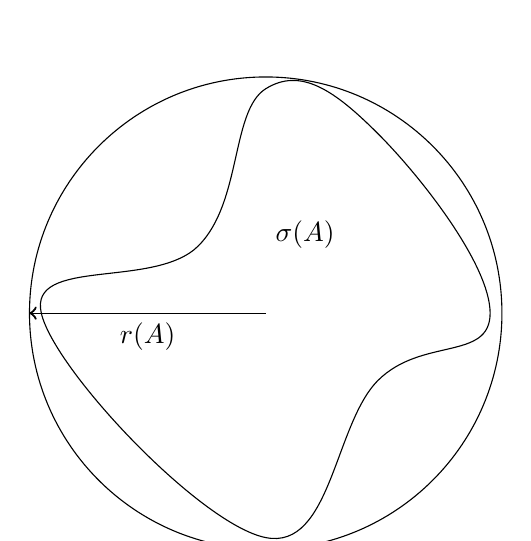
\begin{tikzpicture}[arr/.style={decoration={markings,mark=at position 1 with {\arrow[thick]{>}}},postaction={decorate}}]
\draw (0,0) circle (3);
\draw plot[smooth cycle,tension=.7,scale=2.85] coordinates{(0,-1) (0.5,-0.3) (1,0) (0.5,0.8) (0,1) (-0.3,0.3) (-1,0)};
\node at (0.5,1) {$\sigma(A)$};
\draw[arr] (0,0) -- node [below]{$r(A)$} (-3,0);
\end{tikzpicture}\hfill{}\hspace*{1mm}\caption{$\sigma\left(A\right)\subseteq\overline{B_{r\left(A\right)}\left(0\right)}$}
\end{figure}



\section{Theorem\label{sec:Thm-SpectralRadiusFinite}}

For $A\in L\left(H\right)$ holds:
\begin{align*}
r\left(A\right) & =\limsup_{n\to\infty}\opnorm{A^{n}}^{\frac{1}{n}}
\end{align*}
If $A$ is symmetric, then:
\begin{align*}
r\left(A\right) & =\opnorm A
\end{align*}



\subsubsection*{Proof}

%DATE: Fr 30.11.12

Recall for a power series
\begin{align*}
\sum_{n=0}^{\infty}a_{n}z^{n}
\end{align*}
with $a_{n},z\in\mathbb{K}$ the root test (\foreignlanguage{ngerman}{Wurzelkriterium}):
\begin{itemize}
\item If
\begin{align*}
\limsup_{n\to\infty}\abs{a_{n}z^{n}}^{\frac{1}{n}} & =:c<1
\end{align*}
then $\abs{a_{n}z^{n}}<c^{n}$ and therefore is
\begin{align*}
\sum_{n=0}^{\infty}c^{n}
\end{align*}
a convergent dominating sequence. Thus $\sum_{n=0}^{\infty}a_{n}z^{n}$
converges as well.
\item If
\begin{align*}
\limsup_{n\to\infty}\abs{a_{n}z^{n}}^{\frac{1}{n}} & =:c>1
\end{align*}
then $\abs{a_{n}z^{n}}>c^{n}>1$ for an infinite number of $n$. Therefore
$a_{n}z^{n}$ does \emph{not} converge to zero, which implies that
$\sum_{n=0}^{\infty}a_{n}z^{n}$ does not converge as well.
\item If
\begin{align*}
\limsup_{n\to\infty}\abs{a_{n}z^{n}}^{\frac{1}{n}} & =1
\end{align*}
no conclusion is possible.
\end{itemize}
\begin{align*}
\limsup_{n\to\infty}\abs{a_{n}z^{n}}^{\frac{1}{n}} & =\abs z\cdot\limsup_{n\to\infty}\abs{a_{n}}^{\frac{1}{n}}
\end{align*}
The Radius of convergence (\foreignlanguage{ngerman}{Konvergenzradius})
is thus defined by:
\begin{align*}
R & :=\frac{1}{\limsup_{n\to\infty}\abs{a_{n}}^{\frac{1}{n}}}
\end{align*}
If $\abs z<R$ the sum converges absolutely and if $\abs z>R$ the
sum diverges.\textcolor{green}{}

In our setting for $A=0$ is nothing to prove. For $\lambda\in\varrho\left(A\right)\setminus\left\{ 0\right\} $
we make a formal expansion:
\begin{align*}
\mathcal{R}_{\lambda} & =\left(\lambda-A\right)^{-1}=\frac{1}{\lambda}\left(\mathbbm{1}-\frac{A}{\lambda}\right)^{-1}=\frac{1}{\lambda}\sum_{n=0}^{\infty}A^{n}\cdot\left(\frac{1}{\lambda}\right)^{n}
\end{align*}
This is a power series in $\frac{1}{\lambda}$, but the coefficients
are operators.
\begin{align*}
R & :=\frac{1}{\limsup_{n\to\infty}\opnorm{A^{n}}^{\frac{1}{n}}}
\end{align*}
For $\frac{1}{\abs{\lambda}}<R$
\begin{align*}
\opnorm{\sum_{n=0}^{\infty}A^{n}\left(\frac{1}{\lambda}\right)^{n}} & \le\sum_{n=0}^{\infty}\opnorm{A^{n}}\frac{1}{\lambda^{n}}
\end{align*}
converges absolutely and so
\begin{align*}
\sum_{n=0}^{\infty}A^{n}\left(\frac{1}{\lambda}\right)^{n}
\end{align*}
converges in $L\left(H\right)$. Thus the resolvent 
\begin{align*}
\mathcal{R}_{\lambda} & =\left(\lambda-A\right)^{-1}
\end{align*}
exists and $\sigma\left(A\right)\subseteq\overline{B_{\frac{1}{R}}\left(0\right)}$,
i.e.:
\begin{align*}
r\left(A\right) & \le\frac{1}{R}=\limsup_{n\to\infty}\opnorm{A^{n}}^{\frac{1}{n}}
\end{align*}
If $\frac{1}{\abs{\lambda}}>R$
\begin{align*}
\opnorm{\sum_{n=0}^{\infty}A^{n}\left(\frac{1}{\lambda}\right)^{n}}
\end{align*}
diverges.

\begin{figure}[H]
\hspace*{1mm}\hfill{}\begin{tikzpicture}[arr/.style={decoration={markings,mark=at position 1 with {\arrow[thick]{>}}},postaction={decorate}}]
  \draw (0,0) circle (3);
  \draw[arr] (0,0) -- node [below]{$r(A)$} (-3,0);
  \draw (0,0) circle (5);
  \draw[arr] (0,0) -- node [left]{$\frac{1}{R}$} (0,-5);
  \draw[yshift=60,xshift=33] plot[smooth cycle,tension=.7,scale=2.85] coordinates{(0,-0.8) (0.5,-0.3) (0.2,0) (-0.3,0.1) (-1,0)};
  \node at (0.7,1) {$\sigma(A)$};
  \draw (0.7,4) node[below]{$\lambda$} circle (0.7);
  \draw (0.7,4) +(-0.1,-0.1) -- +(0.1,0.1) +(0.1,-0.1) -- +(-0.1,0.1);
  \draw (0.7,4) -- node[above]{$\delta$} (0,4);
  \draw (0,0) +(-0.1,-0.1) -- +(0.1,0.1) +(0.1,-0.1) -- +(-0.1,0.1);
  \draw (1,4.1) node[above]{$\nu$} +(-0.1,-0.1) -- +(0.1,0.1) +(0.1,-0.1) -- +(-0.1,0.1);
\end{tikzpicture}\hfill{}\hspace*{1mm}\caption{$\frac{1}{R}>r\left(A\right)$ ?}
\end{figure}
Why is $r$ not smaller than $\frac{1}{R}$?\\
Assume that $r<\frac{1}{R}$ and choose $\lambda$ with $r<\abs{\lambda}<\frac{1}{R}$.
Then $\mathcal{R}_{\lambda}$ exists and is analytic. Consider a $\nu\in B_{\delta}\left(\lambda\right)$.
\begin{align*}
\mathcal{R}_{\nu} & =\left(\nu-A\right)^{-1}=\left(\left(\nu-\lambda\right)+\left(\lambda-A\right)\right)^{-1}=\\
 & =\left(\left(\left(\nu-\lambda\right)\mathcal{R}_{\lambda}+\mathbbm{1}\right)\left(\lambda-A\right)\right)^{-1}=\\
 & =\mathcal{R}_{\lambda}\left(\mathbbm{1}+\left(\nu-\lambda\right)\mathcal{R}_{\lambda}\right)^{-1}=\\
 & =\mathcal{R}_{\lambda}\sum_{n=0}^{\infty}\left(-\left(\nu-\lambda\right)\right)^{n}\mathcal{R}_{\lambda}^{n}
\end{align*}
For $\abs{\nu-\lambda}<\delta:=\frac{1}{\opnorm{\mathcal{R}_{\lambda}}}$
the Neumann series converges.\\
Thus $\mathcal{R}_{\lambda}$ can be expanded locally in a power series,
i.e. $\mathcal{R}_{\lambda}$ is complex analytic or holomorphic.\\
Furthermore for $\abs{\lambda}>\frac{1}{R}$ holds: 
\begin{align*}
\mathcal{R}_{\lambda} & =\sum_{n=0}^{\infty}A^{n}\frac{1}{\lambda^{n+1}}
\end{align*}


\begin{figure}[H]
\hspace*{1mm}\hfill{}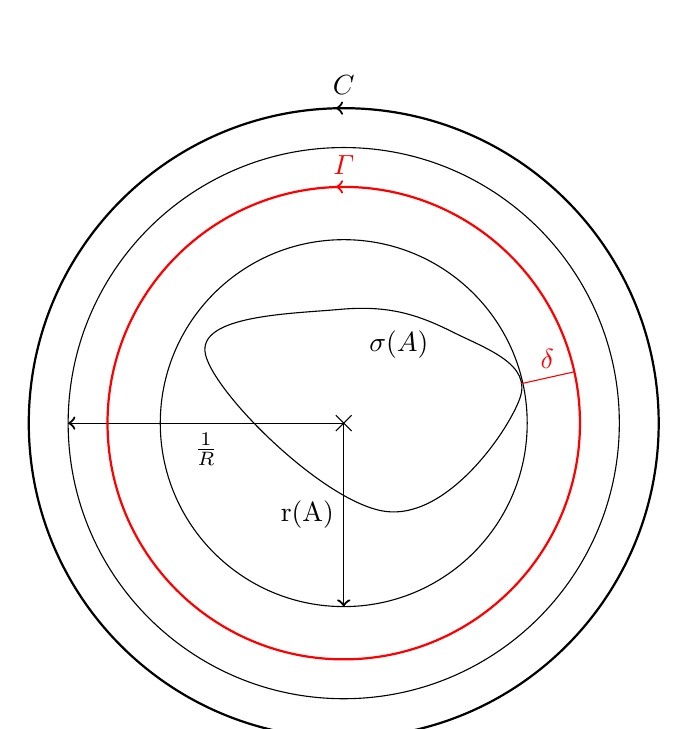
\begin{tikzpicture}[arr/.style={decoration={markings,mark=at position 1 with {\arrow[thick]{>}}},postaction={decorate}}]
  \draw (0,0) circle (3.5);
  \draw (0,0) circle (2.33);
  \draw[arr] (0,0) -- node[left]{r(A)} (0,-2.33);
  \draw[arr] (0,0) -- node [below]{$\frac{1}{R}$} (-3.5,0);
  \draw[yshift=33,xshift=23] plot[smooth cycle,tension=.7,scale=2.85] coordinates{(-0.1,-0.8) (0.5,-0.3) (0.2,0) (-0.3,0.1) (-0.9,-0.1)};
  \node at (0.7,1) {$\sigma(A)$};
  \draw (0,0) +(-0.1,-0.1) -- +(0.1,0.1) +(0.1,-0.1) -- +(-0.1,0.1);
  \draw[red,thick] (0,0) circle (3) node[above=86]{$\Gamma$};
  \draw[red,thick,arr] (0,3) -- (-0.1,3);
  \draw[thick] (0,0) circle (4) node[above=115]{$C$};
  \draw[thick,arr] (0,4) -- (-0.1,4);
  \draw[red] (2.25,0.5) -- node[above]{$\delta$} (2.92,0.65);
\end{tikzpicture}\hfill{}\hspace*{1mm}\caption{Contours $\Gamma$ and $C$ for integration}
\end{figure}


Integrate along the contour $C$:
\begin{align*}
\frac{1}{2\pi\ii}\oint_{C}\lambda^{n}\mathcal{R}_{\lambda}\dd\lambda & =\sum_{k=0}^{\infty}A^{k}\underbrace{\frac{1}{2\pi\ii}\oint_{C}\frac{\lambda^{n}}{\lambda^{k+1}}\dd\lambda}_{=:I}
\end{align*}
Since the geometric series converges absolutely, the summation and
the integration can be interchanged. The residue theorem gives:
\begin{alignat*}{1}
I & =\begin{cases}
1 & \text{if }k=n\\
0 & \text{otherwise}
\end{cases}
\end{alignat*}
Therefore we get:
\begin{align*}
\frac{1}{2\pi\ii}\oint_{C}\lambda^{n}\mathcal{R}_{\lambda}\dd\lambda & =A^{n}
\end{align*}
Choose $\Gamma=\partial B_{r+\delta}\left(0\right)$. We know, that
$\mathcal{R}_{\lambda}$ is holomorphic outside $\Gamma$. Thus we
may continuously deform the contour to obtain:
\begin{align*}
\frac{1}{2\pi\ii}\oint_{\Gamma}\lambda^{n}\mathcal{R}_{\lambda}\dd\lambda & =A^{n}
\end{align*}
Thus we have:
\begin{align*}
\opnorm{A^{n}} & =\opnorm{\frac{1}{2\pi\ii}\oint_{\Gamma}\lambda^{n}\mathcal{R}_{\lambda}\dd\lambda}\le C\left(r+\delta\right)^{n}\left(r+\delta\right)
\end{align*}
\begin{align*}
C & :=\frac{1}{2\pi}\sup_{\lambda\in\Gamma}\opnorm{\mathcal{R}_{\lambda}}
\end{align*}
\begin{align*}
\Rightarrow\quad\opnorm{A^{n}}^{\frac{1}{n}} & \le\left(r+\delta\right)\left(C^{\frac{1}{n}}\left(r+\delta\right)^{\frac{1}{n}}\right)\xrightarrow{n\to\infty}r+\delta
\end{align*}
Therefore:
\begin{align*}
\limsup_{n\to\infty}\opnorm{A^{n}}^{\frac{1}{n}} & \le r+\delta
\end{align*}
Since $\delta$ is arbitrary, it follows that:
\begin{align*}
\frac{1}{R}=\limsup_{n\to\infty}\opnorm{A^{n}}^{\frac{1}{n}} & =r
\end{align*}
We even conclude:
\begin{align*}
\opnorm{A^{n}}^{\frac{1}{n}} & \xrightarrow{n\to\infty}r\left(A\right)
\end{align*}
Assume that $A$ is \emph{symmetric} (to show $\opnorm{A^{n}}^{\frac{1}{n}}=\opnorm A$).
The Schwarz inequality gives:
\begin{align*}
\opnorm{A^{2}} & \le\opnorm A\cdot\opnorm A=\opnorm A^{2}
\end{align*}
\begin{align*}
\opnorm A^{2} & =\sup_{\norm u=1}\left\langle Au,Au\right\rangle =\sup_{\norm u=1}\left\langle u,Au^{2}\right\rangle \le\sup_{\norm u=1}\underbrace{\norm u}_{=1}\cdot\norm{A^{2}u}
\end{align*}
Iteratively for $n\in\mathbb{N}$:
\begin{align*}
\opnorm{A^{2^{n}}} & =\opnorm A^{2^{n}}
\end{align*}
For arbitrary $m\in\mathbb{N}$ the Schwarz inequality gives:
\begin{align*}
\opnorm{A^{m}} & \le\opnorm A^{m}
\end{align*}
Choose $n$ such that $2^{n}>m$. THen:
\begin{align*}
\opnorm A^{2^{n}} & =\opnorm{A^{2^{n}}}=\opnorm{A^{m}\cdot A^{2^{n}-m}}\le\opnorm{A^{m}}\cdot\opnorm A^{2^{n}-m}\\
\Rightarrow\quad\opnorm A^{m} & \le\opnorm A^{m}
\end{align*}
\qqed


\section{Ritz method}

Let $A\in L\left(H\right)$ be a symmetric compact operator on the
separable Hilbert space $H$.\\
From the Hilbert-Schmidt theorem \ref{sec:Thm-Hilbert-Schmidt} we
know that there exists an orthonormal eigenvalue basis $\left(u_{n}\right)$
of $H$. 
\begin{align*}
Au_{n} & =\lambda_{n}u_{n}
\end{align*}
We now want to construct the $u_{n}$:

Consider the ``expectation value'' functional:
\begin{align*}
S:H & \to\mathbb{R}\\
u & \mapsto\left\langle u,Au\right\rangle 
\end{align*}
This is well defined, since:
\begin{align*}
\overline{S\left(u\right)} & =\overline{\left\langle u,Au\right\rangle }=\left\langle Au,u\right\rangle =\left\langle u,Au\right\rangle =S\left(u\right)
\end{align*}
$S$ is bounded, because:
\begin{align*}
\abs{S\left(u\right)} & =\abs{\left\langle u,Au\right\rangle }\le\opnorm A\cdot\norm u^{2}\stackrel{\norm u\le1}{\le}\opnorm A
\end{align*}
Maximize $\abs{S\left(u\right)}$ on $\left\{ u\in H\big|\norm u=1\right\} $:\\
Choose a maximizing sequence $\left(u_{n}\right)$ with $\norm{u_{n}}=1$
and:
\begin{align*}
\abs{S\left(u_{n}\right)} & \xrightarrow{n\to\infty}\sup_{\norm u=1}\abs{S\left(u\right)}
\end{align*}
Since $\overline{B_{1}\left(0\right)}$ is weakly compact, there is
a subsequence $u_{k_{l}}$, which converges weakly $u_{k_{l}}\rightharpoondown u$.\\
Since $A$ is compact, the sequence
\begin{align*}
v_{k_{l}} & :=Au_{k_{l}}\to v
\end{align*}
converges and $Au=v$. As a consequence:
\begin{align*}
S\left(u_{k_{l}}\right) & =\left\langle u_{k_{l}},Au_{k_{l}}\right\rangle =\left\langle u_{k_{l}},v_{k_{l}}\right\rangle =\underbrace{\left\langle u_{k_{l}},v\right\rangle }_{\to\left\langle u,v\right\rangle }+\left\langle u_{k_{l}},v_{k_{l}}-v\right\rangle \xrightarrow{l\to\infty}\left\langle u,v\right\rangle =\left\langle u,Au\right\rangle =S\left(u\right)
\end{align*}
This follows, because:
\begin{align*}
\abs{\left\langle u_{k_{l}},v_{k_{l}}-v\right\rangle } & \le\underbrace{\norm{u_{k_{l}}}}_{=1}\cdot\underbrace{\norm{v_{k_{l}}-v}}_{\to0}\xrightarrow{l\to\infty}0
\end{align*}
Thus $S$ is weakly continuous, i.e. for any $u_{k}\rightharpoondown u$
converges $S\left(u_{k}\right)\to S\left(u\right)$.\\
Because $\left(u_{n}\right)$ is a maximizing sequence, we get:
\begin{align*}
\abs{S\left(u\right)} & =\sup_{\norm{\tilde{u}}=1}\abs{S\left(\tilde{u}\right)}
\end{align*}
Therefore $u$ is the desired maximizer.
\begin{itemize}
\item $u$ is on the unit sphere:\\
The simple approach
\begin{align*}
\norm u^{2} & \not=\lim_{l\to\infty}\norm{u_{k_{l}}}^{2}
\end{align*}
does not work, because $u_{k_{l}}$ only converges weakly.\\
Example:\\
If $\left(e_{l}\right)$ is an orthonormal Hilbert basis in a separable
Hilbert space, then $e_{l}\rightharpoondown0$, but:
\begin{align*}
\lim_{l\to\infty}\norm{e_{l}} & =1\not=0=\norm 0
\end{align*}
But it holds:
\begin{align*}
\norm u^{2} & =\lim_{l\to\infty}\abs{\left\langle u,u_{k_{l}}\right\rangle }\le\lim_{l\to\infty}\norm{u_{k_{l}}}\cdot\norm u=\norm u\\
\Rightarrow\quad\norm u & \le1
\end{align*}
Assume $\norm u<1$, then the vector $\hat{u}:=\frac{u}{\norm u}$
would satisfy the equation:
\begin{align*}
\abs{S\left(\hat{u}\right)} & =\abs{\left\langle \hat{u},A\hat{u}\right\rangle }=\frac{1}{\norm u^{2}}\abs{\left\langle u,Au\right\rangle }=\frac{1}{\norm u^{2}}\sup_{\norm v=1}\abs{S\left(v\right)}\stackrel{\norm u<1}{>}\sup_{\norm v=1}\abs{S\left(v\right)}
\end{align*}
This is a contradiction. Therefore $u$ is in fact a unit vector.%DATE: Do 6.12.12
\item $u$ is an eigenvector corresponding to the eigenvalue $\lambda=\left\langle u,Au\right\rangle \in\mathbb{R}$:
Consider the variation for $v\in H$:
\begin{align*}
\tilde{u}\left(\tau\right) & =u+\tau v
\end{align*}
\begin{align*}
S\left(\frac{\tilde{u}}{\norm{\tilde{u}}}\right) & =\frac{\left\langle \tilde{u},A\tilde{u}\right\rangle }{\left\langle \tilde{u},\tilde{u}\right\rangle }=\frac{\left\langle u+\tau v,A\left(u+\tau v\right)\right\rangle }{\left\langle u+\tau v,u+\tau v\right\rangle }
\end{align*}
This is called \emph{Rayleigh quotient}. We know that $S\left(\tilde{u}\left(\tau\right)\right)$
is extremal at $\tau=0$:
\begin{align*}
0 & =\frac{\dd}{\dd\tau}S\left(\tilde{u}\left(\tau\right)\right)\bigg|_{\tau=0}=\\
 & =\frac{\left\langle u,Av\right\rangle +\left\langle v,Au\right\rangle +2\tau\left\langle v,v\right\rangle }{\left\langle u+\tau v,u+\tau v\right\rangle }-\frac{\left\langle u+\tau v,A\left(u+\tau v\right)\right\rangle }{\left\langle u+\tau v,u+\tau v\right\rangle ^{2}}\cdot\left(\left\langle v,u\right\rangle +\left\langle u,v\right\rangle +\tau\left\langle v,v\right\rangle \right)\bigg|_{\tau=0}=\\
 & \stackrel{A\text{ symmetric}}{=}2\frac{\text{Re}\left(\left\langle v,Au\right\rangle \right)}{\left\langle u,u\right\rangle }-2\text{Re}\left(\left\langle v,u\right\rangle \right)\frac{\left\langle u,Au\right\rangle }{\left\langle u,u\right\rangle ^{2}}=\\
 & \sr ={\lambda=\left\langle u,Au\right\rangle }{\left\langle u,u\right\rangle =1}2\left(\text{Re}\left(\left\langle v,Au\right\rangle \right)-\lambda\text{Re}\left(\left\langle v,u\right\rangle \right)\right)=2\text{Re}\left(\left\langle v,\left(A-\lambda\right)u\right\rangle \right)
\end{align*}
Set $v=e^{\ii\varphi}w$ for any $\varphi\in\mathbb{R}$ and $w\in H$.
So:
\begin{align*}
0 & =\text{Re}\left(\left\langle v,\left(A-\lambda\right)u\right\rangle \right)=\text{Re}\left(e^{-\ii\varphi}\left\langle w,\left(A-\lambda\right)u\right\rangle \right)\qquad\fall_{\varphi\in\mathbb{R}}
\end{align*}
\begin{align*}
\Rightarrow\quad\left\langle w,\left(A-\lambda\right)u\right\rangle  & =0\qquad\fall_{w\in H}\\
\left(A-\lambda\right)u & =0\\
Au & =\lambda u
\end{align*}

\item It holds $\abs{\lambda}=\opnorm A$:\\
There is no point $\nu$ in the spectrum of $A$ with $\abs{\nu}>\abs{\lambda}$,
because otherwise for all $v\in H$ with $Av=\nu v$ follows:
\begin{align*}
\frac{\abs{\left\langle v,Av\right\rangle }}{\left\langle v,v\right\rangle } & =\abs{\nu}>\abs{\lambda}=\abs{\left\langle u,Au\right\rangle }=\sup_{w\in H}\frac{\abs{\left\langle w,Aw\right\rangle }}{\left\langle w,w\right\rangle }
\end{align*}
This is a contradiction. Thus we get:
\begin{align*}
\abs{\lambda} & =\sup_{\nu\in\sigma\left(A\right)}\abs{\nu}\stackrel{\text{by definition}}{=}r\left(A\right)\stackrel{\ref{sec:Thm-SpectralRadiusFinite}}{=}\opnorm A
\end{align*}

\end{itemize}
Thus we have \emph{constructed} a $u\in H$ with $\norm u=1$, $Au=\lambda u$
and $\abs{\lambda}=\opnorm A$. Now one can proceed inductively:
\begin{align*}
H_{1} & :=\left\langle u\right\rangle ^{\perp}
\end{align*}
\begin{align*}
A\big|_{H_{1}}:H_{1} & \to H_{1}
\end{align*}
(We saw that $H_{1}$ is invariant under $A$.)\\
Repeat the above procedure to maximize $\abs{\left\langle v,Av\right\rangle }$
on $H_{1}\cap\left\{ v\in H\big|\norm v=1\right\} $. This gives $u_{1}$
with $\norm u_{1}=1$, $Au_{1}=\lambda_{1}u_{1}$ and:
\begin{align*}
\abs{\lambda_{1}} & =\opnorm{A\big|_{H_{1}}}\le\opnorm{A\big|_{H}}=\abs{\lambda}
\end{align*}
Now set $H_{2}=\left\langle u,u_{1}\right\rangle ^{\perp}$ and proceed
inductively.\\
This gives a sequence $u_{0}:=u,\ u_{1},\ u_{2},\ \ldots$ of orthonormal
eigenvectors, i.e. $Au_{j}=\lambda_{j}u_{j}$, with decreasing eigenvalues$\abs{\lambda_{j}}$.\\
These $\left(u_{j}\right)$ are an orthonormal basis. (Proof as in
Theorem \ref{sec:Thm-Hilbert-Schmidt})\qqed

Ritz, Galerkin: Finite element method\\
Example: Helium molecule wave function in $H=L^{2}\left(\mathbb{R}^{3},\mathbb{C}\right)$

\begin{figure}[H]
\hspace*{1mm}\hfill{}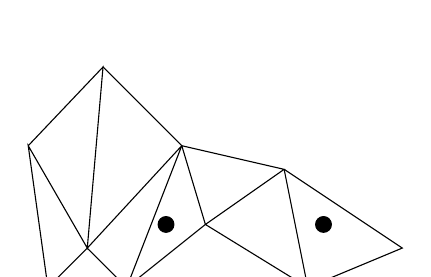
\begin{tikzpicture}
  \draw[fill=black] (-1,0) circle (0.1);
  \draw[fill=black] (1,0) circle (0.1);
  \draw (-2,-0.3) -- (-2.5,-0.8) -- (-2.75,1) -- (-2,-0.3) -- (-1.8,2) -- (-2.75,1);
  \draw (-1.8,2) -- (-0.8,1) -- (-2,-0.3) -- (-1.5,-0.8) -- (-0.8,1);
  \draw (-1.5,-0.8) -- (-2.5,-0.8);
  \draw (-1.5,-0.8) -- (-0.5,0) -- (-0.8,1) -- (0.5,0.7) -- (-0.5,0) -- (0.8,-0.8) -- (2,-0.3) -- (0.5,0.7);
  \draw (0.5,0.7) -- (0.8,-0.8);
\end{tikzpicture}\hfill{}\hspace*{1mm}\caption{finite lattice for numerical approximation}
\end{figure}
\begin{align*}
A & =-\frac{\hbar^{2}}{2m}\Delta-\frac{ze^{2}}{\norm{x-x_{1}}}-\frac{ze^{2}}{\norm{x-x_{2}}}
\end{align*}
Now minimize
\begin{align*}
\frac{\left\langle u,Au\right\rangle }{\left\langle u,u\right\rangle }
\end{align*}
on a finite subspace of $H$.


\chapter{A few (technical) results}


\section{Dini's theorem}

Let $E$ be a metric space and $f_{n}:E\to\mathbb{R}$ a sequence
of real valued functions.


\subsection{Definition \textmd{(point-wise/uniform convergence)}}

$f_{n}$ \emph{converges point-wise} to $f$ if $f_{n}\left(x\right)\to f\left(x\right)$
converges for all $x\in E$, i.e.:
\begin{align*}
\fall_{x\in E}\ \fall_{\varepsilon\in\mathbb{R}_{>0}}\ \exs_{N\left(\varepsilon,x\right)}\ \fall_{n\in\mathbb{N}_{\ge N}}:\  & \abs{f_{n}\left(x\right)-f\left(x\right)}<\varepsilon
\end{align*}


$f_{n}$ \emph{converges uniformly} to $f$, in symbols $f_{n}\rightrightarrows f$,
if for all $\varepsilon\in\mathbb{R}_{>0}$ exists a $N\left(\varepsilon\right)$
such that for all $n\ge N$ and all $x\in E$ holds:
\begin{align*}
\abs{f_{n}\left(x\right)-f\left(x\right)} & <\varepsilon
\end{align*}
With quantifiers this is:
\begin{align*}
\fall_{\varepsilon\in\mathbb{R}_{>0}}\ \exs_{N\left(\varepsilon\right)}\ \fall_{n\in\mathbb{N}_{\ge N}}\ \fall_{x\in E}:\  & \abs{f_{n}\left(x\right)-f\left(x\right)}<\varepsilon
\end{align*}



\subsection{Theorem}

If $\left(f_{n}\right)$ is a sequence of continuous functions with
$f_{n}\rightrightarrows f$, then $f$ is also continuous.\\
This is not true in general for point wise convergence:
\begin{align*}
f_{n}\left(x\right) & =\begin{cases}
1 & \text{for }0\le x\le\frac{1}{2}\left(1-\frac{1}{n}\right)\\
0 & \text{for }x\ge\frac{1}{2}\\
n\left(1-2x\right) & \text{for }\frac{1}{2}\left(1-\frac{1}{n}\right)<x<\frac{1}{2}
\end{cases}
\end{align*}
$f_{n}\to f$ converges pointwise to:
\begin{align*}
f\left(x\right) & =\begin{cases}
1 & x<\frac{1}{2}\\
0 & x\ge\frac{1}{2}
\end{cases}
\end{align*}
This $f$ is \emph{not} continuous.

\begin{figure}[H]
\hspace*{1mm}\hfill{}\begin{tikzpicture}
 \begin{axis}[width=10cm,
			axis x line=middle, axis y line=middle, xmax=1.15, ymax=1.15,
			xlabel=$x$, ylabel=$y$,samples=300]
%  \addplot[domain=0:0.25] {1};
  \addplot[domain=0.25:0.5] {1-4*(x-0.25)};
  \addlegendentry{$f_2(x)$}
  \addplot[domain=0:0.5,red,thick] {1};
  \addlegendentry{$f(x)$}
  \addplot[domain=0.5:1.15,red,thick] {0};
 \end{axis}
 \draw[red, thick, dashed,scale=7.34] (0.5,0) -- (0.5,0.83);
\end{tikzpicture}\hfill{}\hspace*{1mm}\caption{$f_{n}\left(x\right)$ is continuous, but not $f\left(x\right)$}
\end{figure}



\subsubsection*{Proof}

Show that for all $x\in E$ the $\varepsilon$-$\delta$-criterion
is satisfied:\\
Since $f_{n}\rightrightarrows f$ converges uniformly, there is a
$N\in\mathbb{N}$ such that for all $n\in\mathbb{N}_{\ge N}$ and
all $x\in E$ holds:
\begin{align*}
\abs{f_{n}\left(x\right)-f\left(x\right)} & <\frac{\varepsilon}{3}
\end{align*}
Because the $f_{n}$ are continuous, there exists a $\delta\in\mathbb{R}_{>0}$
such that for all $y\in B_{\delta}\left(x\right)$ holds:
\begin{align*}
\abs{f_{N}\left(x\right)-f_{N}\left(y\right)} & <\frac{\varepsilon}{3}
\end{align*}
Now follows for all $y\in B_{\delta}\left(x\right)$:
\begin{align*}
\abs{f\left(y\right)-f\left(x\right)} & \le\underbrace{\abs{f\left(y\right)-f_{N}\left(y\right)}}_{<\frac{\varepsilon}{3}}+\underbrace{\abs{f_{N}\left(y\right)-f_{N}\left(x\right)}}_{<\frac{\varepsilon}{3}}+\underbrace{\abs{f_{N}\left(x\right)-f\left(x\right)}}_{<\frac{\varepsilon}{3}}<\varepsilon
\end{align*}
Therefore $f$ is continuous.\qqed


\subsection{Definition \textmd{(monotonically increasing/decreasing)}}

The sequence of functions $\left(f_{n}\right)$, $f_{n}:E\to\mathbb{R}$
is called \emph{monotonically increasing (decreasing)} if for all
$x\in E$ the real sequence $f_{n}\left(x\right)$ is monotonically
increasing (decreasing).


\subsection{Theorem \textmd{(Dini)}}

Let $E$ be a \emph{compact} metric space, $\left(f_{n}\right)$ monotone
and $f_{n}\to f$.\\
If $f_{n}$ and $f$ are continuous, then the convergence $f_{n}\rightrightarrows f$
is uniform.


\subsubsection*{Proof}

Without loss of generality we assume $\left(f_{n}\right)$ is a monotonically
increasing sequence (otherwise consider $-f_{n}$), i.e. $f_{n}\left(x\right)\le f_{n+1}\left(x\right)$
for all $x\in E$ and all $n\in\mathbb{N}$.\\
Given $\varepsilon>0$ we want to show:
\begin{align*}
\exs_{N\in\mathbb{N}}\ \fall_{x\in E}\ \fall_{\in\mathbb{N}_{\ge N}}:\  & \abs{f\left(x\right)-f_{n}\left(x\right)}<\varepsilon
\end{align*}
For any $x\in E$ there exists an $N\left(x\right)$ such that $\abs{f_{n}\left(x\right)-f\left(x\right)}<\frac{\varepsilon}{2}$
for all $n\in\mathbb{N}_{\ge N}$ (point-wise convergence). Since
both $f_{N\left(x\right)}$ and $f$ are continuous functions, there
exists a neighborhood $U\left(x\right)=B_{\delta\left(x\right)}\left(x\right)$
of $x$ such that for all $z\in U\left(x\right)$ holds:
\begin{align*}
\abs{f_{N\left(x\right)}\left(z\right)-f_{N\left(x\right)}\left(x\right)} & \le\frac{\varepsilon}{4}\\
\abs{f\left(z\right)-f\left(x\right)} & \le\frac{\varepsilon}{4}
\end{align*}
Then follows:
\begin{align*}
\abs{f_{N\left(x\right)}\left(z\right)-f\left(z\right)} & \le\underbrace{\abs{f_{N\left(x\right)}\left(z\right)-f_{N\left(x\right)}\left(x\right)}}_{\le\frac{\varepsilon}{4}}+\underbrace{\abs{f_{N\left(x\right)}\left(x\right)-f\left(x\right)}}_{<\frac{\varepsilon}{2}}+\underbrace{\abs{f\left(x\right)-f\left(z\right)}}_{\le\frac{\varepsilon}{4}}<\varepsilon
\end{align*}
Since $f_{n}\left(z\right)$ is monotonically increasing, it follows
that $\abs{f_{n}\left(z\right)-f\left(z\right)}<\varepsilon$ for
all $z\in B_{\delta\left(x\right)}\left(x\right)$.\\
Now use a standard compactness argument: Since $E$ is compact, it
can be covered by a finite number of these balls $B_{\delta\left(x_{1}\right)}\left(x_{1}\right),\ldots,B_{\delta\left(x_{n}\right)}\left(x_{n}\right)$.
Define:
\begin{align*}
N & =\max\left\{ N\left(x_{1}\right),\ldots,N\left(x_{n}\right)\right\} 
\end{align*}
So for all $n\in\mathbb{N}_{\ge N}$ holds:
\begin{align*}
\abs{f_{n}\left(x\right)-f\left(x\right)} & <\varepsilon
\end{align*}


\qqed


\section{Stone-Weierstraß theorem}

We follow the nice (since constructive) proof by Bernstein.


\subsection{Definition \textmd{(polynomials)}}

Let $E=C^{0}\left(\left[0,1\right]\right)$ be the Banach space of
real valued functions with norm $\norm f=\sup_{x\in\left[0,1\right]}\abs{f\left(x\right)}$.
$\mathcal{P}\left(\left[0,1\right]\right)$ are the \emph{real polynomials},
i.e. for $f\in\mathcal{P}\left(\left[0,1\right]\right)$ there are
$a_{j}\in\mathbb{R}$ such that:
\begin{align*}
f\left(x\right) & =a_{n}x^{n}+a_{n-1}x^{n-1}+\ldots+a_{0}
\end{align*}
Clearly $\mathcal{P}\left(\left[0,1\right]\right)\subseteq C^{0}\left(\left[0,1\right]\right)$
forms a subspace.

We want to show that $\mathcal{P}\left(\left[0,1\right]\right)$ is
dense in $C^{0}\left(\left[0,1\right]\right)$.


\subsection{Lemma}

For $x\in\left[0,1\right]$ holds:

\begin{align*}
\sum_{k=0}^{n}\left(\begin{array}{c}
n\\
k
\end{array}\right)x^{k}\left(1-x\right)^{n-k} & =1
\end{align*}



\subsubsection{Proof}

\begin{align*}
\sum_{k=0}^{n}\left(\begin{array}{c}
n\\
k
\end{array}\right)x^{k}\left(1-x\right)^{n-k} & =\left(x+1-x\right)^{n}=1
\end{align*}
\qqed


\subsection{Lemma}

For $x\in\left[0,1\right]$ holds:

\begin{align*}
\sum_{k=0}^{n}\left(nx-k\right)^{2}\left(\begin{array}{c}
n\\
k
\end{array}\right)x^{k}\left(1-x\right)^{n-k} & =nx\left(1-x\right)\le\frac{n}{4}
\end{align*}
Obviously holds
\begin{align*}
\left(nx-k\right)^{2} & \le4n^{2}
\end{align*}
and therefore:
\begin{align*}
\sum_{k=0}^{n}\left(nx-k\right)^{2}\left(\begin{array}{c}
n\\
k
\end{array}\right)x^{k}\left(1-x\right)^{n-k} & \le4n^{2}\sum_{k=0}^{n}\left(\begin{array}{c}
n\\
k
\end{array}\right)x^{k}\left(1-x\right)^{n-k}=4n^{2}
\end{align*}



\subsubsection{Proof}

It holds:
\begin{align*}
\sum_{k=0}^{n}k\left(\begin{array}{c}
n\\
k
\end{array}\right)x^{k}\left(1-x\right)^{n-k} & =\sum_{k=0}^{n}k\frac{n!}{k!\left(n-k\right)!}x^{k}\left(1-x\right)^{n-k}=\\
 & =0+\sum_{k=1}^{n}\frac{n\cdot\left(n-1\right)!}{\left(k-1\right)!\left(n-k\right)!}x^{k}\left(1-x\right)^{n-k}=\\
 & =n\sum_{k=1}^{n}\left(\begin{array}{c}
n-1\\
k-1
\end{array}\right)x^{k}\left(1-x\right)^{n-k}=\\
 & \sr ={j:=k-1}{}n\sum_{j=0}^{n-1}\left(\begin{array}{c}
n-1\\
j
\end{array}\right)x^{j+1}\left(1-x\right)^{n-j-1}=\\
 & =nx\sum_{j=0}^{n-1}\left(\begin{array}{c}
n-1\\
j
\end{array}\right)x^{j}\left(1-x\right)^{\left(n-1\right)-j}=nx\left(x+1-x\right)^{n-1}=nx
\end{align*}
Similarly one gets:
\begin{align*}
\sum_{k=0}^{n}k\left(k-1\right)\left(\begin{array}{c}
n\\
k
\end{array}\right)x^{k}\left(1-x\right)^{n-k} & =n\left(n-1\right)\sum_{k=2}\left(\begin{array}{c}
n-2\\
k-2
\end{array}\right)x^{k}\left(1-x\right)^{n-k}=n\left(n-1\right)x^{2}
\end{align*}
Together this gives:
\begin{align*}
 & \sum_{k=0}^{n}\left(nx-k\right)^{2}\left(\begin{array}{c}
n\\
k
\end{array}\right)x^{k}\left(1-x\right)^{n-k}=\sum_{k=0}^{n}\left(n^{2}x^{2}-2nxk+k^{2}\right)\left(\begin{array}{c}
n\\
k
\end{array}\right)x^{k}\left(1-x\right)^{n-k}=\\
 & \qquad=\sum_{k=0}^{n}\left(n^{2}x^{2}-2nxk+k\left(k-1\right)+k\right)\left(\begin{array}{c}
n\\
k
\end{array}\right)x^{k}\left(1-x\right)^{n-k}=\\
 & \qquad=n^{2}x^{2}-2nx\cdot nx+n\left(n-1\right)x^{2}+nx=\\
 & \qquad=-n^{2}x^{2}+n^{2}x^{2}-nx^{2}+nx=nx\left(1-x\right)
\end{align*}
\qqed

A more elegant method is to use derivatives:
\begin{align*}
\sum_{k=0}^{n}\left(\begin{array}{c}
n\\
k
\end{array}\right)x^{k}y^{n-k} & =\left(x+y\right)^{n}\\
\sum_{k=0}^{n}k\left(\begin{array}{c}
n\\
k
\end{array}\right)x^{k}y^{n-k} & =x\cdot\frac{\dd}{\dd x}\left(\sum_{k=0}^{n}\left(\begin{array}{c}
n\\
k
\end{array}\right)x^{k}y^{n-k}\right)\\
\sum_{k=0}^{n}k^{2}\left(\begin{array}{c}
n\\
k
\end{array}\right)x^{k}y^{n-k} & =\left(x\cdot\frac{\dd}{\dd x}\right)^{2}\left(\sum_{k=0}^{n}\left(\begin{array}{c}
n\\
k
\end{array}\right)x^{k}y^{n-k}\right)
\end{align*}



\subsection{Definition}

For $f\in C^{0}\left(\left[0,1\right]\right)$ define:
\begin{align*}
B_{n}f\left(x\right) & :=\sum_{k=0}^{n}f\left(\frac{k}{n}\right)\left(\begin{array}{c}
n\\
k
\end{array}\right)x^{k}\left(1-x\right)^{n-k}
\end{align*}



\subsection{Theorem \textmd{(Bernstein)}}

For any $f\in C^{0}\left(\left[0,1\right],\mathbb{R}\right)$, $B_{n}f\rightrightarrows f$
converges uniformly.

Example: $f\left(x\right)=10x\cdot e^{-3x}+\frac{1}{5}\cos\left(\left(4x\right)^{2}\right)$
\begin{align*}
B_{4}f\left(x\right) & \approx0,2\cdot\left(1-x\right)^{4}+5,2\cdot x\cdot\left(1-x\right)^{3}+5,9\cdot x^{2}\cdot\left(1-x\right)^{2}+2,4\cdot x^{3}\cdot\left(1-x\right)+0,3\cdot x^{4}\\
B_{10}f\left(x\right) & \approx0,2\cdot\left(1-x\right)^{10}+9,4\cdot x\cdot\left(1-x\right)^{9}+56,6\cdot x^{2}\cdot\left(1-x\right)^{8}+\\
 & \qquad+149,5\cdot x^{3}\cdot\left(1-x\right)^{7}+217,9\cdot x^{4}\cdot\left(1-x\right)^{6}+248,2\cdot x^{5}\cdot\left(1-x\right)^{5}+\\
 & \qquad+244,7\cdot x^{6}\cdot\left(1-x\right)^{4}+103,2\cdot x^{7}\cdot\left(1-x\right)^{3}+26,5\cdot x^{8}\cdot\left(1-x\right)^{2}+\\
 & \qquad+7,9\cdot x^{9}\cdot\left(1-x\right)+0,3\cdot x^{10}
\end{align*}


\begin{figure}[H]
\hspace*{1mm}\hfill{}\begin{tikzpicture}
 \begin{axis}[width=10cm,
			axis x line=middle, axis y line=middle, xmax=1.15, ymin=0,
			xlabel=$x$, ylabel=$y$,samples=300,domain=0:1]
  \addplot[domain=0:1] {10*exp(-3*x)*x+0.2*cos(16*x^2 r)};
  \addlegendentry{$f(x)$}
  \addplot[red,dotted,thick] {0.2*(1-x)^4+5.1559073721*x*(1-x)^3+5.90953245942*x^2*(1-x)^2 +2.43307252735*x^3*(1-x)+0.306338787614*x^4};
  \addlegendentry{$B_4f(x)$}
  \addplot[green,dashed,thick] {0.2*(1-x)^10 + 9.38263677357*x*(1-x)^9 + 56.6119090694*x^2*(1-x)^8 +
			149.495246516*x^3*(1-x)^7 + 217.908409367*x^4*(1-x)^6 + 248.200363295*x^5*(1-x)^5 +
			244.658345846*x^6*(1-x)^4 + 103.198948015*x^7*(1-x)^3 + 26.4871020479*x^8*(1-x)^2 +
			7.89554238831*x^9*(1-x) + 0.306338787614 *x^10};
  \addlegendentry{$B_{10}f(x)$}
  \addplot[blue,thick] {0.2*(x - 1)^100 - 29.7044297355*(x - 1)^99*x + 1922.32661312*(x - 1)^98*x^2 - 76671.4488442*(x - 1)^97*x^3 + 2175113.86842*(x - 1)^96*x^4 - 47445744.0975*(x - 1)^95*x^5 + 835426611.054*(x - 1)^94*x^6 - 12274511676.0*(x - 1)^93*x^7 + (1.54128159816e+11)*(x - 1)^92*x^8 - (1.68416809261e+12)*(x - 1)^91*x^9 + (1.62416346068e+13)*(x - 1)^90*x^10 - (1.39799905505e+14)*(x - 1)^89*x^11 + (1.08395744118e+15)*(x - 1)^88*x^12 - (7.62894913085e+15)*(x - 1)^87*x^13 + (4.90524281676e+16)*(x - 1)^86*x^14 - (2.89723345963e+17)*(x - 1)^85*x^15 + (1.57938018746e+18)*(x - 1)^84*x^16 - (7.97909365281e+18)*(x - 1)^83*x^17 + (3.74925611597e+19)*(x - 1)^82*x^18 - (1.64375304991e+20)*(x - 1)^81*x^19 + (6.742898184e+20)*(x - 1)^80*x^20 - (2.59454195168e+21)*(x - 1)^79*x^21 + (9.38534683558e+21)*(x - 1)^78*x^22 - (3.19807571697e+22)*(x - 1)^77*x^23 + (1.02840511571e+23)*(x - 1)^76*x^24 - (3.12601722657e+23)*(x - 1)^75*x^25 + (8.99540551127e+23)*(x - 1)^74*x^26 - (2.45384693521e+24)*(x - 1)^73*x^27 + (6.3535833129e+24)*(x - 1)^72*x^28 - (1.56329402068e+25)*(x - 1)^71*x^29 + (3.65918765199e+25)*(x - 1)^70*x^30 - (8.15630256136e+25)*(x - 1)^69*x^31 + (1.7329494044e+26)*(x - 1)^68*x^32 - (3.51288267659e+26)*(x - 1)^67*x^33 + (6.80009456156e+26)*(x - 1)^66*x^34 - (1.25811363872e+27)*(x - 1)^65*x^35 + (2.22666269336e+27)*(x - 1)^64*x^36 - (3.7730643047e+27)*(x - 1)^63*x^37 + (6.12656303633e+27)*(x - 1)^62*x^38 - (9.54121434063e+27)*(x - 1)^61*x^39 + (1.42639048452e+28)*(x - 1)^60*x^40 - (2.04882695285e+28)*(x - 1)^59*x^41 + (2.82997586185e+28)*(x - 1)^58*x^42 - (3.76214352396e+28)*(x - 1)^57*x^43 + (4.81728554268e+28)*(x - 1)^56*x^44 - (5.94543941083e+28)*(x - 1)^55*x^45 + (7.0766223624e+28)*(x - 1)^54*x^46 - (8.12653547869e+28)*(x - 1)^53*x^47 + (9.0056905284e+28)*(x - 1)^52*x^48 - (9.6308442906e+28)*(x - 1)^51*x^49 + (9.93701125777e+28)*(x - 1)^50*x^50 - (9.88794489827e+28)*(x - 1)^49*x^51 + (9.48295145921e+28)*(x - 1)^48*x^52 - (8.75834176186e+28)*(x - 1)^47*x^53 + (7.78277250071e+28)*(x - 1)^46*x^54 - (6.64705004092e+28)*(x - 1)^45*x^55 + (5.45033587088e+28)*(x - 1)^44*x^56 - (4.28565344267e+28)*(x - 1)^43*x^57 + (3.22776989136e+28)*(x - 1)^42*x^58 - (2.32579971336e+28)*(x - 1)^41*x^59 + (1.60149090844e+28)*(x - 1)^40*x^60 - (1.05260827225e+28)*(x - 1)^39*x^61 + (6.59659001145e+27)*(x - 1)^38*x^62 - (3.93748270015e+27)*(x - 1)^37*x^63 + (2.23625120007e+27)*(x - 1)^36*x^64 - (1.2072827702e+27)*(x - 1)^35*x^65 + (6.19022488168e+26)*(x - 1)^34*x^66 - (3.01225494685e+26)*(x - 1)^33*x^67 + (1.39035634551e+26)*(x - 1)^32*x^68 - (6.08541276274e+25)*(x - 1)^31*x^69 + (2.52599547528e+25)*(x - 1)^30*x^70 - (9.95022718871e+24)*(x - 1)^29*x^71 + (3.72450252857e+24)*(x - 1)^28*x^72 - (1.32760664266e+24)*(x - 1)^27*x^73 + (4.51994903095e+23)*(x - 1)^26*x^74 - (1.47516743127e+23)*(x - 1)^25*x^75 + (4.63264469906e+22)*(x - 1)^24*x^76 - (1.40412004325e+22)*(x - 1)^23*x^77 + (4.11230568962e+21)*(x - 1)^22*x^78 - (1.16208158162e+21)*(x - 1)^21*x^79 + (3.15481027286e+20)*(x - 1)^20*x^80 - (8.17300500354e+19)*(x - 1)^19*x^81 + (2.00415639672e+19)*(x - 1)^18*x^82 - (4.6119830604e+18)*(x - 1)^17*x^83 + (9.87622406444e+17)*(x - 1)^16*x^84 - (1.95242968902e+17)*(x - 1)^15*x^85 + (3.53637476861e+16)*(x - 1)^14*x^86 - (5.82579078166e+15)*(x - 1)^13*x^87 + (8.66482439273e+14)*(x - 1)^12*x^88 - (1.15456063319e+14)*(x - 1)^11*x^89 + (1.36674282068e+13)*(x - 1)^10*x^90 - (1.4240167171e+12)*(x - 1)^9*x^91 + (1.29209648425e+11)*(x - 1)^8*x^92 - 10086134970.2*(x - 1)^7*x^93 + 667798780.604*(x - 1)^6*x^94 - 36881544.6299*(x - 1)^5*x^95 + 1664862.88706*(x - 1)^4*x^96 - 59769.1901049*(x - 1)^3*x^97 + 1631.70663884*(x - 1)^2*x^98 - 30.797227045*(x - 1)*x^99 + 0.306338787614*x^100};
  \addlegendentry{$B_{100}f(x)$}
  \addplot[mark=x, samples=100, only marks, blue] {10*exp(-3*x)*x+0.2*cos(16*x^2 r)};
  \addplot[mark=*, samples=10, only marks, green] {10*exp(-3*x)*x+0.2*cos(16*x^2 r)};
  \addplot[mark=triangle*, samples=4, only marks, red] {10*exp(-3*x)*x+0.2*cos(16*x^2 r)};
 \end{axis}
\end{tikzpicture}\hfill{}\hspace*{1mm}\caption{Approximation of $f\left(x\right)$ by $B_{n}f\left(x\right)$}
\end{figure}



\subsubsection*{Proof}

Without loss of generality assume $f\not=0$ (otherwise $B_{n}f=0=f$).
\begin{align*}
M & :=\norm f>0
\end{align*}
Consider an arbitrary $\varepsilon\in\mathbb{R}_{>0}$. $f$ is continuous
on the compact set $\left[0,1\right]$ and thus uniformly continuous,
i.e. there exists a $\delta\in\mathbb{R}_{>0}$ such that:
\begin{align*}
\abs{x-y} & <\delta\quad\Rightarrow\qquad\abs{f\left(x\right)-f\left(y\right)}<\frac{\varepsilon}{2}
\end{align*}
Choose $\mathbb{N}\ni N\ge\frac{M}{\varepsilon\delta^{2}}$.
\begin{description}
\item [{Claim:}] $\abs{B_{n}f\left(x\right)-f\left(x\right)}<\varepsilon$
for all $x\in\left[0,1\right]$ and all $n\ge N$.
\item [{Proof:}] It holds:
\begin{align*}
f\left(x\right) & =\sum_{k=0}^{n}f\left(x\right)\left(\begin{array}{c}
n\\
k
\end{array}\right)x^{k}\left(1-x\right)^{n-k}\\
B_{n}f\left(x\right) & =\sum_{k=0}^{n}f\left(\frac{k}{n}\right)\left(\begin{array}{c}
n\\
k
\end{array}\right)x^{k}\left(1-x\right)^{n-k}
\end{align*}
\begin{align*}
\left(B_{n}f-f\right)\left(x\right) & =\sum_{k=0}^{\infty}\left(f\left(\frac{k}{n}\right)-f\left(x\right)\right)\left(\begin{array}{c}
n\\
k
\end{array}\right)x^{k}\left(1-x\right)^{n-k}
\end{align*}
Define:
\begin{align*}
A & :=\left\{ k\Bigg|\abs{\frac{k}{n}-x}<\delta\right\}  & B & :=\left\{ k\Bigg|\abs{\frac{k}{n}-x}\ge\delta\right\} 
\end{align*}
We have:
\begin{align*}
\sum_{k\in A}\underbrace{\abs{f\left(\frac{k}{n}\right)-f\left(x\right)}}_{<\frac{\varepsilon}{2}}\left(\begin{array}{c}
n\\
k
\end{array}\right)x^{k}\left(1-x\right)^{n-k} & <\frac{\varepsilon}{2}\sum_{k\in A}\left(\begin{array}{c}
n\\
k
\end{array}\right)x^{k}\left(1-x\right)^{n-k}\le\frac{\varepsilon}{2}
\end{align*}
\begin{align*}
 & \sum_{k\in B}\underbrace{\abs{f\left(\frac{k}{n}\right)-f\left(x\right)}}_{\le2\norm f=2M}\left(\begin{array}{c}
n\\
k
\end{array}\right)x^{k}\left(1-x\right)^{n-k}\le\\
 & \qquad\le2M\sum_{k\in B}\left(\begin{array}{c}
n\\
k
\end{array}\right)x^{k}\left(1-x\right)^{n-k}\le\\
 & \qquad\sr{\le}{k\in B}{\Rightarrow n^{2}\delta^{2}\le\left(k-nx\right)^{2}}\frac{2M}{n^{2}\delta^{2}}\sum_{k=0}^{n}\underbrace{\left(k-nx\right)^{2}\left(\begin{array}{c}
n\\
k
\end{array}\right)x^{k}\left(1-x\right)^{n-k}}_{\le\frac{n}{4}}\le\\
 & \qquad\stackrel{n\ge N}{\le}\frac{M}{2n\delta^{2}}\le\frac{M}{2\frac{M}{\varepsilon\delta^{2}}\delta^{2}}=\frac{\varepsilon}{2}
\end{align*}
Therefore holds for all $x\in\left[0,1\right]$.
\begin{align*}
\abs{B_{n}f\left(x\right)-f\left(x\right)} & <\frac{\varepsilon}{2}+\frac{\varepsilon}{2}=\varepsilon
\end{align*}
\qqed[Claim]
\end{description}
Therefore $B_{n}f\rightrightarrows f$ converges uniformly.\qqed

%DATE: Fr 07.12.12

Now generalize: Let $E$ be a compact metric space. $C^{0}\left(E,\mathbb{R}\right)$
with
\begin{align*}
\norm f & =\sup_{x\in E}\abs{f\left(x\right)}
\end{align*}
is a Banach space. Moreover, it is an algebra with the point-wise
multiplication:
\begin{align*}
\left(f\cdot g\right)\left(x\right) & :=f\left(x\right)\cdot g\left(x\right)
\end{align*}
The multiplication is continuous:
\begin{align*}
\norm{f\cdot g} & \le\norm f\cdot\norm g
\end{align*}
In summary $\left(C^{0}\left(E,\mathbb{R}\right),\norm .,+,\cdot\right)$
is a \emph{Banach algebra}.


\subsection{Theorem \textmd{(Weierstraß)\label{sub:Thm-Weierstra=0000DF}}}

The polynomials are dense in $C^{0}\left(\left[0,1\right],\mathbb{R}\right)$.


\subsubsection*{Proof}

For any $f\in C^{0}\left(\left[0,1\right],\mathbb{R}\right)$, $B_{n}f\rightrightarrows f$
converges uniformly and since the $B_{n}f$ are polynomials, these
are dense.\qqed


\subsection{Theorem \textmd{(Stone-Weierstraß)\label{sub:Thm-Stone-Weierstra=0000DF}}}

Let $\mathcal{A}\subseteq C^{0}\left(E,\mathbb{R}\right)$ be a subalgebra
with the following properties:
\begin{enumerate}
\item $\mathcal{A}$ contains $f=1$ and so by scalar multiplication all
the constant functions.
\item $\mathcal{A}$ separates the points of $E$, i.e. for all $x,y\in E$
with $x\not=y$ there exists a $f\in\mathcal{A}$ such that $f\left(x\right)\not=f\left(y\right)$.
\end{enumerate}
Then $\mathcal{A}$ is dense in $C^{0}\left(E,\mathbb{R}\right)$.


\subsubsection*{Proof}
\begin{enumerate}[label=\roman*)]
\item There is a sequence of polynomials $u_{n}$ on $\left[0,1\right]$
such that $u_{n}\rightrightarrows f$ with $f\left(t\right)=\sqrt{t}$.
This follows immediately from theorem \ref{sub:Thm-Weierstra=0000DF}.
\item If $f\in\mathcal{A}$, then $\abs f$ defined by $\abs f\left(x\right):=\abs{f\left(x\right)}$
is in the closure $\overline{\mathcal{A}}$ of $\mathcal{A}$:\\
For $f\in\mathcal{A}$ define:
\begin{align*}
a & :=\norm f=\max_{x\in E}\abs{f\left(x\right)}
\end{align*}
\begin{align*}
\Rightarrow\quad\frac{f^{2}\left(x\right)}{a^{2}} & \in\left[0,1\right]
\end{align*}
Then converges:
\begin{align*}
u_{n}\left(\frac{f^{2}\left(x\right)}{a^{2}}\right) & \xrightarrow{n\to\infty}\sqrt{\frac{f^{2}\left(x\right)}{a^{2}}}=\frac{\abs{f\left(x\right)}}{a}
\end{align*}
The functions $u_{n}\left(\frac{f^{2}}{a^{2}}\right)$ lie in $\mathcal{A}$,
since these are a polynomials of $f$ and thus again elements of the
algebra $\mathcal{A}$. Moreover $u_{n}\left(\frac{f^{2}}{a^{2}}\right)$
converges uniformly to $\frac{\abs f}{a}$, because for a given $\varepsilon\in\mathbb{R}_{>0}$
exists a $N\in\mathbb{N}$ such that for all $n\in\mathbb{N}_{\ge N}$
and all $t\in\left[0,1\right]$ holds:
\begin{align*}
\abs{u_{n}\left(t\right)-\sqrt{t}} & <\varepsilon
\end{align*}
Then follows with $t=\frac{f^{2}\left(x\right)}{a^{2}}$:
\begin{align*}
\abs{u_{n}\left(\frac{f^{2}\left(x\right)}{a^{2}}\right)-\frac{\abs f}{a}} & <\varepsilon
\end{align*}
Thus $\frac{\abs f}{a}\in\overline{\mathcal{A}}$ and therefore also
$\abs f\in\overline{\mathcal{A}}$.
\item For $f,g\in\overline{\mathcal{A}}$ also $\min\left(f,g\right)$ and
$\max\left(f,g\right)$ (defined point-wise) are again in $\overline{\mathcal{A}}$:
\begin{align*}
\min\left(f,g\right) & =\frac{1}{2}\left(f+g-\abs{f-g}\right)\\
\max\left(f,g\right) & =\frac{1}{2}\left(f+g+\abs{f-g}\right)
\end{align*}
Choose $f_{n},g_{n}\in\mathcal{A}$ such that $f_{n}\rightrightarrows f$
and $g_{n}\rightrightarrows g$. By ii) follows $\abs{f_{n}-g_{n}}\in\overline{\mathcal{A}}$
and $\abs{f_{n}-g_{n}}\rightrightarrows\abs{f-g}$. Therefore holds:
\begin{align*}
\overline{\mathcal{A}}\ni\min\left(f_{n},g_{n}\right) & \rightrightarrows\min\left(f,g\right)\in\overline{\mathcal{A}}
\end{align*}
Similarly the claim follows for $\max$.
\item For all $x,y\in E$ with $x\not=y$ and $\alpha,\beta\in\mathbb{R}$
exists a $f\in\mathcal{A}$ such that $f\left(x\right)=\alpha$ and
$f\left(y\right)=\beta$:\\
For $\alpha=\beta$ we choose $f=\alpha$ as constant function.\\
For $\alpha\not=\beta$ there exists, since $\mathcal{A}$ separates
points of $E$, a $g\in\mathcal{A}$ with $g\left(x\right)\not=g\left(y\right)$.
Set $f=c_{0}+c_{1}g$ and choose:
\begin{align*}
\alpha & =c_{0}+c_{1}g\left(x\right)\\
\beta & =c_{0}+c_{1}g\left(y\right)\\
\Rightarrow\quad c_{1} & =\frac{\alpha-\beta}{g\left(x\right)-g\left(y\right)}\\
\Rightarrow\quad c_{0} & =\alpha-\frac{\alpha-\beta}{g\left(x\right)-g\left(y\right)}g\left(x\right)=\frac{\alpha g\left(x\right)-\alpha g\left(y\right)-\alpha g\left(x\right)+\beta g\left(x\right)}{g\left(x\right)-g\left(y\right)}=\\
 & =\frac{\beta g\left(x\right)-\alpha g\left(y\right)}{g\left(x\right)-g\left(y\right)}
\end{align*}

\item For all $f\in C^{0}$, $x\in E$ and $\varepsilon\in\mathbb{R}_{>0}$
there is a $g\in\overline{\mathcal{A}}$ such that
\begin{align*}
g\left(x\right) & =f\left(x\right)
\end{align*}
and for all $y\in\overline{\mathcal{A}}$ holds:
\begin{align*}
g\left(y\right) & \le f\left(y\right)+\varepsilon
\end{align*}
\begin{figure}[H]
\hspace*{1mm}\hfill{}\begin{tikzpicture}
 \begin{axis}[width=10cm,
			axis x line=middle, axis y line=middle, xmax=1.15, ymin=0, ymax=1.2, ytick=0,
			samples=300,domain=0:1]
  \addplot[domain=0:1] {0.5+0.3*sin(x*180)};
  \addlegendentry{$f(x)$}
  \addplot[red,dashed,thick] {0.6+0.3*sin(x*180)};
  \addlegendentry{$f(x)+\varepsilon$}
  \addplot[blue,dotted,thick] {0.5+0.3*sin(x*180)+0.07*exp(-x)*cos(10*x^2 r)};
  \addlegendentry{$g(x)$}
 \end{axis}
  \draw[dashed] (5.05,0) -- (5.05,4.42);
  \draw (5.05,0) -- (5.05,-0.1) node[below] {$x$};
\end{tikzpicture}\hfill{}\hspace*{1mm}\caption{$g\left(x\right)\le f\left(x\right)+\varepsilon$}
\end{figure}
To show this, choose for any $z\in E$ a $h_{z}\in\overline{\mathcal{A}}$
with $h_{z}\left(x\right)=f\left(x\right)$ and $h_{z}\left(z\right)\le f\left(z\right)+\frac{\varepsilon}{2}$,
which is possible after iv).\\
Since $h_{z}$ is continuous, there is a neighborhood $U_{z}$ of
$z$ such that $h_{z}\le f+\varepsilon$ on $U_{z}$.
\begin{figure}[H]
\hspace*{1mm}\hfill{}\begin{tikzpicture}
 \begin{axis}[width=10cm,
			axis x line=middle, axis y line=middle, xmax=1.15, ymin=0, ymax=1.2, ytick={}, xtick={0,0.5,1},
			samples=300,domain=0:1]
  \addplot[domain=0:1] {0.5+0.3*sin(x*180)};
  \addlegendentry{$f(x)$}
  \addplot[red,dashed,thick] {0.6+0.3*sin(x*180)};
  \addlegendentry{$f(x)+\varepsilon$}
  \addplot[blue,dotted,thick] {0.5+0.3*sin(x*180)+0.1*(exp(-x)*cos(10*x^2 r)-1) + 0.05 + 0.5*x*sin(x^2*360)};
  \addlegendentry{$h_z(x)$}
 \end{axis}
  \draw[dashed] (5.05,0) -- (5.05,4.42);
  \draw (5.05,0) -- (5.05,-0.1) node[below] {$x$};
  \draw[dashed] (0.8,0) -- (0.8,3.5);
  \draw (0.8,0) -- (0.8,-0.1) node[below] {$z$};
  \draw[red,thick] (0.2,0) -- node[above right]{$U_z$} (1.6,0);
  \draw[red,thick] (0.2,0.1) -- (0.2,-0.1) (1.6,0.1) -- (1.6,-0.1);
\end{tikzpicture}\hfill{}\hspace*{1mm}\caption{$h_{z}\le f+\varepsilon$ on $U_{z}$}
\end{figure}
Since $E$ is compact, we can cover it by a finite number of such
neighborhoods $U_{z_{1}},\ldots,U_{z_{N}}$. Define:
\begin{align*}
g & :=\min\left\{ h_{z_{1}},\ldots,h_{z_{N}}\right\} \in\overline{\mathcal{A}}
\end{align*}
It holds $g\left(x\right)=f\left(x\right)$, because $h_{z_{i}}\left(x\right)=f\left(x\right)$.
We also know:
\begin{align*}
g\big|_{U_{j}} & \le h_{z_{j}}\big|_{U_{j}}\le f+\varepsilon
\end{align*}

\item $\overline{\mathcal{A}}=C^{0}$: Denote the function $g$ constructed
in step v) by $g_{x}$.
\begin{align*}
g_{x}\left(x\right) & =f\left(x\right)\\
g_{x} & \le f+\varepsilon
\end{align*}
By continuity of $g_{x}$ there exists a neighborhood $U_{x}$ of
$x$ such that $g_{x}\ge f-\varepsilon$ on $U_{x}$. By compactness
we can cover $E$ by a finite number of such neighborhoods $U_{x_{1}},\ldots,U_{x_{k}}$
and define:
\begin{align*}
g & :=\max\left\{ g_{x_{1}},\ldots,g_{x_{k}}\right\} 
\end{align*}
Then follows:
\begin{align*}
f-\varepsilon\le & g\le f+\varepsilon\\
\norm{f-g} & <\varepsilon
\end{align*}
\qqed
\end{enumerate}
Counterexample in the complex case:
\begin{align*}
E & =\left[0,1\right]\times\left[0,1\right]\subseteq\mathbb{C}
\end{align*}
Consider the set $\mathcal{A}=\mathcal{P}\left(z\right)$ of polynomials
in $z$.
\begin{itemize}
\item The constant functions are in $\mathcal{A}$.
\item $\mathcal{A}$ separates points:\\
If $z_{1}\not=z_{2}$ take $f\left(z\right)=z$ then $f\left(z_{1}\right)\not=f\left(z_{2}\right)$.
\begin{align*}
\overline{\mathcal{A}} & =?
\end{align*}
By Morera's theorem we get:
\begin{align*}
\overline{\mathcal{A}} & =\left\{ f\in C^{0}\left(\left[0,1\right]^{2}\right)\bigg|\big|f\big|_{\left(0,1\right)^{2}}\text{ is holomorphic}\right\} \not=C^{0}\left(\left[0,1\right]^{2}\right)
\end{align*}
For example $f\left(x+\ii y\right)=x-\ii y$. We have $f\in C^{0}\left(\left[0,1\right]^{2}\right)$,
but $f\not\in\overline{\mathcal{A}}$.
\end{itemize}

\subsection{Theorem \textmd{(Stone-Weierstraß, complex version)}}

Let $\mathcal{A}\subseteq C^{0}\left(E,\mathbb{C}\right)$ be a subalgebra
with the properties 1. and 2. from theorem \ref{sub:Thm-Stone-Weierstra=0000DF}
and additionally:
\begin{enumerate}
\item [3.]$f\in\mathcal{A}\Rightarrow\overline{f}\in\mathcal{A}$
\end{enumerate}
Then $\mathcal{A}$ is dense in $C^{0}\left(E,\mathbb{C}\right)$.


\subsubsection*{Proof}

Consider the algebras:
\begin{align*}
\text{Re}\left(\mathcal{A}\right) & =\left\{ f+\overline{f}\Big|f\in\mathcal{A}\right\} \subseteq\mathcal{A}\\
\text{Im}\left(\mathcal{A}\right) & =\left\{ \frac{1}{\ii}\left(f-\overline{f}\right)\bigg|f\in\mathcal{A}\right\} \subseteq\mathcal{A}
\end{align*}
These are subalgebras of $C^{0}\left(E,\mathbb{R}\right)$. By the
real Stone-Weierstraß theorem we get:
\begin{align*}
\overline{\text{Re}\left(\mathcal{A}\right)} & =\overline{\text{Im}\left(\mathcal{A}\right)}=C^{0}\left(E,\mathbb{R}\right)
\end{align*}
For given $f\in C^{0}\left(E,\mathbb{C}\right)$ approximate $\text{Re}\left(f\right)$
and $\text{Im}\left(f\right)$.\qqed


\section{Arzelà-Ascoli theorem}

Let $K$ be a compact metric space and $E$ a Banach space.

$C^{0}\left(K,E\right)$ is the Banach space of continuous functions
$f:K\to E$ with norm:
\begin{align*}
\norm f & :=\sup_{x\in K}\norm{f\left(x\right)}_{E}
\end{align*}
Let $\mathcal{F}\subseteq C^{0}\left(K,E\right)$ be a subset. Is
$\mathcal{F}$ compact?


\subsection{Definition \textmd{(relatively compact)}}

A subset $A$ of a metric space is called \emph{relatively compact},
if $\overline{A}$ is compact.


\subsection{Definition \textmd{(equicontinuous)}}

A family $\mathcal{F}\subseteq C^{0}\left(K,E\right)$ is called \emph{equicontinuous}
(\foreignlanguage{ngerman}{gleichgradig stetig}) if for all $x\in K$
and all $\varepsilon\in\mathbb{R}_{>0}$ there exists a $\delta\in\mathbb{R}_{>0}$
such that for all $y\in B_{\delta}\left(x\right)$ and for all $f\in\mathcal{F}$
holds:
\begin{align*}
\norm{f\left(x\right)-f\left(y\right)} & <\varepsilon
\end{align*}
(Thus $\delta$ is independent of $f\in\mathcal{F}$.)


\subsection{Theorem \textmd{(Arzelà-Ascoli)}}

$\mathcal{F}\subseteq C^{0}\left(K,E\right)$ is relatively compact
if and only if the following two conditions holds:
\begin{enumerate}[label=\roman*)]
\item $\mathcal{F}$ is equicontinuous.
\item For every $x\in K$ the set
\begin{align*}
\mathcal{F}\left(x\right) & :=\left\{ f\left(x\right)\big|f\in\mathcal{F}\right\} 
\end{align*}
is relatively compact in $E$.
\end{enumerate}

\subsubsection*{Proof}

„$\Rightarrow$“: Assume that $\mathcal{F}\subseteq C^{0}\left(K,E\right)$
is relatively compact.
\begin{enumerate}[label=\roman*)]
\item Assume that $\mathcal{F}$ is \emph{not} equicontinuous. Then there
exists an $\varepsilon\in\mathbb{R}_{>0}$ and sequences $x_{n}\in K$,
$f_{n}\in\mathcal{F}$ and $y_{n}\in B_{\frac{1}{n}}\left(x_{n}\right)$
such that:
\begin{align*}
\norm{f_{n}\left(x_{n}\right)-f_{n}\left(y_{n}\right)} & \ge\varepsilon
\end{align*}
After choosing subsequences (with the same notation), we can arrange:
\begin{align*}
x_{n} & \to x & y_{n} & \to x &  & \left(\text{use that }K\text{ is compact}\right)\\
f_{n} & \to f &  &  &  & \left(\text{use that }\mathcal{F}\text{ is relatively compact}\right)
\end{align*}
This means that there is a $N\in\mathbb{N}$ such that for all $n\in\mathbb{N}_{>N}$
holds for all $y\in K$:
\begin{align*}
\norm{f_{n}\left(y\right)-f\left(y\right)} & <\frac{\varepsilon}{3}
\end{align*}
(Since convergence in $C^{0}\left(K,E\right)$ is the same as uniform
convergence $f_{n}\rightrightarrows f$.)\\
Since $f$ is continuous there exists a $\delta\in\mathbb{R}_{>0}$
such that for all $y\in B_{\delta}\left(x\right)$:
\begin{align*}
\norm{f\left(x\right)-f\left(y\right)} & <\frac{\varepsilon}{3}
\end{align*}
With this we get:
\begin{align*}
\norm{f_{n}\left(x\right)-f_{n}\left(y\right)} & \le\underbrace{\norm{f_{n}\left(x\right)-f\left(x\right)}}_{<\frac{\varepsilon}{3}}+\underbrace{\norm{f\left(x\right)-f\left(y\right)}}_{<\frac{\varepsilon}{3}}+\underbrace{\norm{f\left(y\right)-f_{n}\left(y\right)}}_{<\frac{\varepsilon}{3}}<\varepsilon
\end{align*}
This is a contradiction to $\norm{f_{n}\left(x_{n}\right)-f_{n}\left(y_{n}\right)}\ge\varepsilon$.\qqed[\roman{enumi})]
\item Consider $y_{n}\in\mathcal{F}\left(x\right)\subseteq E$ (to show
that $y_{n}$ has a convergent subsequence in $E$).\\
Then there are functions $f_{n}\in\mathcal{F}$ with $f_{n}\left(x\right)=y_{n}$.
Since $\mathcal{F}$ is relatively compact, a subsequence is a Cauchy
sequence in $C^{0}\left(K,E\right)$, i.e. $\norm{f_{n_{l}}\to f_{n_{l'}}}\xrightarrow{l,l'\to\infty}0$.
\begin{align*}
\norm{f_{n_{l}}-f_{n_{l'}}} & =\sup_{z\in K}\norm{f_{n_{l}}\left(z\right)-f_{n_{l'}}\left(z\right)}_{E}\ge\norm{f_{n_{l}}\left(x\right)-f_{n_{l'}}\left(x\right)}_{E}=\norm{y_{n_{l}}-y_{n_{l'}}}
\end{align*}
Therefore we get+:
\begin{align*}
\norm{y_{n_{l}}-y_{n_{l'}}} & \xrightarrow{l,l'\to\infty}0
\end{align*}
Thus $\left(y_{n_{l}}\right)$ is a Cauchy sequence in $E$.\qqed[\roman{enumi})]
\end{enumerate}

\section{Riesz representation theorem}


\part*{Appendix\thispagestyle{empty}}

\addcontentsline{toc}{part}{Appendix}

\fancyhead[R]{}
\fancyhead[C]{Appendix}


\chapter*{Acknowledgements}

\addcontentsline{toc}{section}{\hspace*{2.7em}Acknowledgements}

\fancyhead[R]{Acknowledgements}

My special thanks goes to Professor Finster, who gave this lecture
and allowed me to publish this script of the lecture.

I would also like to thank all those, who found errors by careful
reading and told me of them.

\vspace{1cm}


\hfill{}Andreas Völklein


\chapter*{GNU Free Documentation License}

\addcontentsline{toc}{section}{\hspace*{2.7em}GNU Free Documentation License}

\fancyhead[R]{GNU Free Documentation License}

\noindent \begin{center}
Version 1.3, 3 November 2008\\
Copyright © 2000, 2001, 2002, 2007, 2008 Free Software Foundation,
Inc. 
\par\end{center}

\noindent \begin{center}
\texttt{<}\url{https://fsf.org/}\texttt{>}
\par\end{center}

\noindent \begin{center}
Everyone is permitted to copy and distribute verbatim copies of this
license document,\\
but changing it is not allowed
\par\end{center}


\section*{\noun{0. Preamble}}

\noindent The purpose of this License is to make a manual, textbook,
or other functional and useful document “free” in the sense of freedom:
to assure everyone the effective freedom to copy and redistribute
it, with or without modifying it, either commercially or noncommercially.
Secondarily, this License preserves for the author and publisher a
way to get credit for their work, while not being considered responsible
for modifications made by others.

\noindent This License is a kind of “copyleft”, which means that derivative
works of the document must themselves be free in the same sense. It
complements the GNU General Public License, which is a copyleft license
designed for free software.

\noindent We have designed this License in order to use it for manuals
for free software, because free software needs free documentation:
a free program should come with manuals providing the same freedoms
that the software does. But this License is not limited to software
manuals; it can be used for any textual work, regardless of subject
matter or whether it is published as a printed book. We recommend
this License principally for works whose purpose is instruction or
reference.


\section*{\noun{1. Applicability and definitions}}

This License applies to any manual or other work, in any medium, that
contains a notice placed by the copyright holder saying it can be
distributed under the terms of this License. Such a notice grants
a world-wide, royalty-free license, unlimited in duration, to use
that work under the conditions stated herein. The “\textbf{Document}”,
below, refers to any such manual or work. Any member of the public
is a licensee, and is addressed as “\textbf{you}”. You accept the
license if you copy, modify or distribute the work in a way requiring
permission under copyright law.

A “\textbf{Modified Version}” of the Document means any work containing
the Document or a portion of it, either copied verbatim, or with modifications
and/or translated into another language.

A “\textbf{Secondary Section}” is a named appendix or a front-matter
section of the Document that deals exclusively with the relationship
of the publishers or authors of the Document to the Document's overall
subject (or to related matters) and contains nothing that could fall
directly within that overall subject. (Thus, if the Document is in
part a textbook of mathematics, a Secondary Section may not explain
any mathematics.) The relationship could be a matter of historical
connection with the subject or with related matters, or of legal,
commercial, philosophical, ethical or political position regarding
them.

The “\textbf{Invariant Sections}” are certain Secondary Sections whose
titles are designated, as being those of Invariant Sections, in the
notice that says that the Document is released under this License.
If a section does not fit the above definition of Secondary then it
is not allowed to be designated as Invariant. The Document may contain
zero Invariant Sections. If the Document does not identify any Invariant
Sections then there are none.

The “\textbf{Cover Texts}” are certain short passages of text that
are listed, as Front-Cover Texts or Back-Cover Texts, in the notice
that says that the Document is released under this License. A Front-Cover
Text may be at most 5 words, and a Back-Cover Text may be at most
25 words.

A “\textbf{Transparent}” copy of the Document means a machine-readable
copy, represented in a format whose specification is available to
the general public, that is suitable for revising the document straightforwardly
with generic text editors or (for images composed of pixels) generic
paint programs or (for drawings) some widely available drawing editor,
and that is suitable for input to text formatters or for automatic
translation to a variety of formats suitable for input to text formatters.
A copy made in an otherwise Transparent file format whose markup,
or absence of markup, has been arranged to thwart or discourage subsequent
modification by readers is not Transparent. An image format is not
Transparent if used for any substantial amount of text. A copy that
is not “Transparent” is called “\textbf{Opaque}”.

Examples of suitable formats for Transparent copies include plain
ASCII without markup, Texinfo input format, \LaTeX{} input format,
SGML or XML using a publicly available DTD, and standard-conforming
simple HTML, PostScript or PDF designed for human modification. Examples
of transparent image formats include PNG, XCF and JPG. Opaque formats
include proprietary formats that can be read and edited only by proprietary
word processors, SGML or XML for which the DTD and/or processing tools
are not generally available, and the machine-generated HTML, PostScript
or PDF produced by some word processors for output purposes only.

The “\textbf{Title Page}” means, for a printed book, the title page
itself, plus such following pages as are needed to hold, legibly,
the material this License requires to appear in the title page. For
works in formats which do not have any title page as such, “Title
Page” means the text near the most prominent appearance of the work's
title, preceding the beginning of the body of the text.

The “\textbf{publisher}” means any person or entity that distributes
copies of the Document to the public.

A section “\textbf{Entitled XYZ}” means a named subunit of the Document
whose title either is precisely XYZ or contains XYZ in parentheses
following text that translates XYZ in another language. (Here XYZ
stands for a specific section name mentioned below, such as “\textbf{Acknowledgements}”,
“\textbf{Dedications}”, “\textbf{Endorsements}”, or “\textbf{History}”.)
To “\textbf{Preserve the Title}” of such a section when you modify
the Document means that it remains a section “Entitled XYZ” according
to this definition.

The Document may include Warranty Disclaimers next to the notice which
states that this License applies to the Document. These Warranty Disclaimers
are considered to be included by reference in this License, but only
as regards disclaiming warranties: any other implication that these
Warranty Disclaimers may have is void and has no effect on the meaning
of this License.


\section*{\noun{2. Verbatim copying}}

You may copy and distribute the Document in any medium, either commercially
or noncommercially, provided that this License, the copyright notices,
and the license notice saying this License applies to the Document
are reproduced in all copies, and that you add no other conditions
whatsoever to those of this License. You may not use technical measures
to obstruct or control the reading or further copying of the copies
you make or distribute. However, you may accept compensation in exchange
for copies. If you distribute a large enough number of copies you
must also follow the conditions in section 3.

You may also lend copies, under the same conditions stated above,
and you may publicly display copies.


\section*{\noun{3. Copying in quantity}}

If you publish printed copies (or copies in media that commonly have
printed covers) of the Document, numbering more than 100, and the
Document's license notice requires Cover Texts, you must enclose the
copies in covers that carry, clearly and legibly, all these Cover
Texts: Front-Cover Texts on the front cover, and Back-Cover Texts
on the back cover. Both covers must also clearly and legibly identify
you as the publisher of these copies. The front cover must present
the full title with all words of the title equally prominent and visible.
You may add other material on the covers in addition. Copying with
changes limited to the covers, as long as they preserve the title
of the Document and satisfy these conditions, can be treated as verbatim
copying in other respects.

If the required texts for either cover are too voluminous to fit legibly,
you should put the first ones listed (as many as fit reasonably) on
the actual cover, and continue the rest onto adjacent pages.

If you publish or distribute Opaque copies of the Document numbering
more than 100, you must either include a machine-readable Transparent
copy along with each Opaque copy, or state in or with each Opaque
copy a computer-network location from which the general network-using
public has access to download using public-standard network protocols
a complete Transparent copy of the Document, free of added material.
If you use the latter option, you must take reasonably prudent steps,
when you begin distribution of Opaque copies in quantity, to ensure
that this Transparent copy will remain thus accessible at the stated
location until at least one year after the last time you distribute
an Opaque copy (directly or through your agents or retailers) of that
edition to the public.

It is requested, but not required, that you contact the authors of
the Document well before redistributing any large number of copies,
to give them a chance to provide you with an updated version of the
Document.


\section*{\noun{4. Modifications}}

You may copy and distribute a Modified Version of the Document under
the conditions of sections 2 and 3 above, provided that you release
the Modified Version under precisely this License, with the Modified
Version filling the role of the Document, thus licensing distribution
and modification of the Modified Version to whoever possesses a copy
of it. In addition, you must do these things in the Modified Version:
\begin{description}
\item [{A.\hspace*{3.2mm}}] Use in the Title Page (and on the covers,
if any) a title distinct from that of the Document, and from those
of previous versions (which should, if there were any, be listed in
the History section of the Document). You may use the same title as
a previous version if the original publisher of that version gives
permission.
\item [{B.\hspace*{3.4mm}}] List on the Title Page, as authors, one or
more persons or entities responsible for authorship of the modifications
in the Modified Version, together with at least five of the principal
authors of the Document (all of its principal authors, if it has fewer
than five), unless they release you from this requirement.
\item [{C.\hspace*{3.4mm}}] State on the Title page the name of the publisher
of the Modified Version, as the publisher.
\item [{D.\hspace*{3.4mm}}] Preserve all the copyright notices of the
Document.
\item [{E.\hspace*{3.4mm}}] Add an appropriate copyright notice for your
modifications adjacent to the other copyright notices.
\item [{F.\hspace*{3.8mm}}] Include, immediately after the copyright notices,
a license notice giving the public permission to use the Modified
Version under the terms of this License, in the form shown in the
Addendum below.
\item [{G.\hspace*{3.1mm}}] Preserve in that license notice the full lists
of Invariant Sections and required Cover Texts given in the Document's
license notice.
\item [{H.\hspace*{3.2mm}}] Include an unaltered copy of this License.
\item [{I.\hspace*{5.0mm}}] Preserve the section Entitled “History”, Preserve
its Title, and add to it an item stating at least the title, year,
new authors, and publisher of the Modified Version as given on the
Title Page. If there is no section Entitled “History” in the Document,
create one stating the title, year, authors, and publisher of the
Document as given on its Title Page, then add an item describing the
Modified Version as stated in the previous sentence.
\item [{J.\hspace*{4.3mm}}] Preserve the network location, if any, given
in the Document for public access to a Transparent copy of the Document,
and likewise the network locations given in the Document for previous
versions it was based on. These may be placed in the “History” section.
You may omit a network location for a work that was published at least
four years before the Document itself, or if the original publisher
of the version it refers to gives permission.
\item [{K.\hspace*{3.3mm}}] For any section Entitled “Acknowledgements”
or “Dedications”, Preserve the Title of the section, and preserve
in the section all the substance and tone of each of the contributor
acknowledgements and/or dedications given therein.
\item [{L.\hspace*{4.1mm}}] Preserve all the Invariant Sections of the
Document, unaltered in their text and in their titles. Section numbers
or the equivalent are not considered part of the section titles.
\item [{M.\hspace*{3mm}}] Delete any section Entitled “Endorsements”.
Such a section may not be included in the Modified Version.
\item [{N.\hspace*{3.4mm}}] Do not retitle any existing section to be
Entitled “Endorsements” or to conflict in title with any Invariant
Section.
\item [{O.\hspace*{3.4mm}}] Preserve any Warranty Disclaimers.
\end{description}
If the Modified Version includes new front-matter sections or appendices
that qualify as Secondary Sections and contain no material copied
from the Document, you may at your option designate some or all of
these sections as invariant. To do this, add their titles to the list
of Invariant Sections in the Modified Version's license notice. These
titles must be distinct from any other section titles.

You may add a section Entitled “Endorsements”, provided it contains
nothing but endorsements of your Modified Version by various parties—for
example, statements of peer review or that the text has been approved
by an organization as the authoritative definition of a standard.

You may add a passage of up to five words as a Front-Cover Text, and
a passage of up to 25 words as a Back-Cover Text, to the end of the
list of Cover Texts in the Modified Version. Only one passage of Front-Cover
Text and one of Back-Cover Text may be added by (or through arrangements
made by) any one entity. If the Document already includes a cover
text for the same cover, previously added by you or by arrangement
made by the same entity you are acting on behalf of, you may not add
another; but you may replace the old one, on explicit permission from
the previous publisher that added the old one.

The author(s) and publisher(s) of the Document do not by this License
give permission to use their names for publicity for or to assert
or imply endorsement of any Modified Version.


\section*{\noun{5. Combining documents}}

You may combine the Document with other documents released under this
License, under the terms defined in section 4 above for modified versions,
provided that you include in the combination all of the Invariant
Sections of all of the original documents, unmodified, and list them
all as Invariant Sections of your combined work in its license notice,
and that you preserve all their Warranty Disclaimers.

The combined work need only contain one copy of this License, and
multiple identical Invariant Sections may be replaced with a single
copy. If there are multiple Invariant Sections with the same name
but different contents, make the title of each such section unique
by adding at the end of it, in parentheses, the name of the original
author or publisher of that section if known, or else a unique number.
Make the same adjustment to the section titles in the list of Invariant
Sections in the license notice of the combined work.

In the combination, you must combine any sections Entitled “History”
in the various original documents, forming one section Entitled “History”;
likewise combine any sections Entitled “Acknowledgements”, and any
sections Entitled “Dedications”. You must delete all sections Entitled
“Endorsements”.


\section*{\noun{6. Collections of documents}}

You may make a collection consisting of the Document and other documents
released under this License, and replace the individual copies of
this License in the various documents with a single copy that is included
in the collection, provided that you follow the rules of this License
for verbatim copying of each of the documents in all other respects.

You may extract a single document from such a collection, and distribute
it individually under this License, provided you insert a copy of
this License into the extracted document, and follow this License
in all other respects regarding verbatim copying of that document.


\section*{\noun{7. Aggregation with independent works}}

A compilation of the Document or its derivatives with other separate
and independent documents or works, in or on a volume of a storage
or distribution medium, is called an “aggregate” if the copyright
resulting from the compilation is not used to limit the legal rights
of the compilation's users beyond what the individual works permit.
When the Document is included in an aggregate, this License does not
apply to the other works in the aggregate which are not themselves
derivative works of the Document.

If the Cover Text requirement of section 3 is applicable to these
copies of the Document, then if the Document is less than one half
of the entire aggregate, the Document's Cover Texts may be placed
on covers that bracket the Document within the aggregate, or the electronic
equivalent of covers if the Document is in electronic form. Otherwise
they must appear on printed covers that bracket the whole aggregate.


\section*{\noun{8. Translation}}

Translation is considered a kind of modification, so you may distribute
translations of the Document under the terms of section 4. Replacing
Invariant Sections with translations requires special permission from
their copyright holders, but you may include translations of some
or all Invariant Sections in addition to the original versions of
these Invariant Sections. You may include a translation of this License,
and all the license notices in the Document, and any Warranty Disclaimers,
provided that you also include the original English version of this
License and the original versions of those notices and disclaimers.
In case of a disagreement between the translation and the original
version of this License or a notice or disclaimer, the original version
will prevail.

If a section in the Document is Entitled “Acknowledgements”, “Dedications”,
or “History”, the requirement (section 4) to Preserve its Title (section
1) will typically require changing the actual title.


\section*{\noun{9. Termination}}

You may not copy, modify, sublicense, or distribute the Document except
as expressly provided under this License. Any attempt otherwise to
copy, modify, sublicense, or distribute it is void, and will automatically
terminate your rights under this License.

However, if you cease all violation of this License, then your license
from a particular copyright holder is reinstated (a) provisionally,
unless and until the copyright holder explicitly and finally terminates
your license, and (b) permanently, if the copyright holder fails to
notify you of the violation by some reasonable means prior to 60 days
after the cessation.

Moreover, your license from a particular copyright holder is reinstated
permanently if the copyright holder notifies you of the violation
by some reasonable means, this is the first time you have received
notice of violation of this License (for any work) from that copyright
holder, and you cure the violation prior to 30 days after your receipt
of the notice.

Termination of your rights under this section does not terminate the
licenses of parties who have received copies or rights from you under
this License. If your rights have been terminated and not permanently
reinstated, receipt of a copy of some or all of the same material
does not give you any rights to use it.


\section*{\noun{10. Future revisions of this license}}

The Free Software Foundation may publish new, revised versions of
the GNU Free Documentation License from time to time. Such new versions
will be similar in spirit to the present version, but may differ in
detail to address new problems or concerns. See \url{https://www.gnu.org/copyleft/}.

Each version of the License is given a distinguishing version number.
If the Document specifies that a particular numbered version of this
License \textquotedbl{}or any later version\textquotedbl{} applies
to it, you have the option of following the terms and conditions either
of that specified version or of any later version that has been published
(not as a draft) by the Free Software Foundation. If the Document
does not specify a version number of this License, you may choose
any version ever published (not as a draft) by the Free Software Foundation.
If the Document specifies that a proxy can decide which future versions
of this License can be used, that proxy's public statement of acceptance
of a version permanently authorizes you to choose that version for
the Document.


\section*{\noun{11. Relicensing}}

“Massive Multiauthor Collaboration Site” (or “MMC Site”) means any
World Wide Web server that publishes copyrightable works and also
provides prominent facilities for anybody to edit those works. A public
wiki that anybody can edit is an example of such a server. A “Massive
Multiauthor Collaboration” (or “MMC”) contained in the site means
any set of copyrightable works thus published on the MMC site.

“CC-BY-SA” means the Creative Commons Attribution-Share Alike 3.0
license published by Creative Commons Corporation, a not-for-profit
corporation with a principal place of business in San Francisco, California,
as well as future copyleft versions of that license published by that
same organization.

“Incorporate” means to publish or republish a Document, in whole or
in part, as part of another Document.

An MMC is “eligible for relicensing” if it is licensed under this
License, and if all works that were first published under this License
somewhere other than this MMC, and subsequently incorporated in whole
or in part into the MMC, (1) had no cover texts or invariant sections,
and (2) were thus incorporated prior to November 1, 2008.

The operator of an MMC Site may republish an MMC contained in the
site under CC-BY-SA on the same site at any time before August 1,
2009, provided the MMC is eligible for relicensing.


\section*{\noun{Addendum}: How to use this License for your documents}

To use this License in a document you have written, include a copy
of the License in the document and put the following copyright and
license notices just after the title page:
\begin{quote}
Copyright © YEAR YOUR NAME.\\
Permission is granted to copy, distribute and/or modify this document
under the terms of the GNU Free Documentation License, Version 1.3
or any later version published by the Free Software Foundation;

with no Invariant Sections, no Front-Cover Texts, and no Back-Cover
Texts.

A copy of the license is included in the section entitled \textquotedbl{}GNU
Free Documentation License\textquotedbl{}.
\end{quote}
If you have Invariant Sections, Front-Cover Texts and Back-Cover Texts,
replace the \textquotedbl{}with $\ldots$ Texts.\textquotedbl{} line
with this:
\begin{quote}
with the Invariant Sections being LIST THEIR TITLES, with the Front-Cover
Texts being LIST, and with the Back-Cover Texts being LIST.
\end{quote}
If you have Invariant Sections without Cover Texts, or some other
combination of the three, merge those two alternatives to suit the
situation.

If your document contains nontrivial examples of program code, we
recommend releasing these examples in parallel under your choice of
free software license, such as the GNU General Public License, to
permit their use in free software.

\label{END}
\end{document}
